\section{Compiling Ladder Operator Block-Encodings}
\label{sec:ladder-op-oracles}

In this work, we focus on generating block-encodings for second-quantized operators that act on both fermionic and bosonic modes.
In this section, we provide a framework for compiling controlled block-encodings of products and linear combinations of fermionic and bosonic ladder operators.

The framework for generating these block-encodings primarily relies on infering the action of the operators on the fermionic and bosonic modes upon which the operator acts nontrivially. 
The compilations presented below are optimized primarily to reduce the number of non-Clifford operations and secondarily to reduce the number of block-encoding ancillae.

Although controlled applications of block-encodings are not always required in quantum algorithms, control qubits are included throughout this section to demonstrate that controlling the block-encoding does not significantly affect the cost of the block-encoding.
For applications that do not require a controlled application of the block-encoding, the control qubits can simply be omitted and the cost associated with the uncontrolled block-encoding will be reduced accordingly.

\subsection{Encoding}
\label{subsec:encoding}

The Jordan-Wigner transformation \cite{jordan-wigner} maps fermionic ladder operators to Pauli operators acting on qubits.
Under this transformation, Fock states of fermionic modes are represented by qubit states using the following map:
\begin{equation}
    \ket{\psi_{{I_b - 1}} \dots \psi_{1_b} \psi_{0_b}} \rightarrow \ket{q_{{I_b - 1}} \dots q_{1_b} q_{0_b}}
\end{equation}
where $\psi_{i_b} = q_{i_b} \in [0, 1]$ depending on if the $i^\text{th}$ fermionic mode is occupied ($\ket{1}$) or unoccupied ($\ket{0}$).
In this work, we use the same qubit encoding to represent the occupation of fermionic modes.
The number of qubits required for the fermionic system is equal to the number of fermionic modes.

The encoding scheme for bosons must be able to represent a number of bosons in the range $\psi_{i_a} \in [0, \Omega]$ for each bosonic mode.
We choose to represent store the occupancy of a bosonic mode in binary notation following \cite{rhodes2024exponential}:
\begin{equation}
    \ket{\psi_{i_a}} \rightarrow \ket{q_{i_a}^{w-1} \hdots q_{i_a}^{1} q_{i_a}^0}
\end{equation}
where the subscript denotes the index of the bosonic mode and the superscripts denote the index of the qubit storing the $w^{th}$ least-significant bit of the binary representation of $\psi_{i_a}$.
Due to the binary encoding, the number of qubits needed to represent each mode is $w = \lceil \log_2{(\Omega + 1)} \rceil$.
Fock states of multiple bosonic modes can be expressed as follows:
\begin{equation}
    \begin{split}
        &\ket{\psi_{I_a - 1}} \otimes \hdots \otimes \ket{\psi_{1_a}} \otimes \ket{\psi_{0_a}} \rightarrow \\
        &\ket{q_{I_a - 1}^{w-1} \hdots q_{I_a - 1}^{1} q_{I_a - 1}^0} \otimes \hdots \\
        \otimes &\ket{q_{1}^{w-1} \hdots q_{1}^{1} q_{1}^0} \otimes \ket{q_{0}^{w-1} \hdots q_{0}^{1} q_{0}^0} \\
    \end{split}
\end{equation}
In this work, we assume that the maximum bosonic occupancy for each bosonic mode is identical.
However, this encoding scheme and the block-encoding constructions presented below can be easily adapted to allow for bosonic modes to have different maximum occupation numbers.

\subsection{Fermionic Ladder Operators}
\label{subsec:fermionic-be}

Here, we construct block-encodings for the individual fermionic creation ($b_j^\dagger$) and annihilation ($b_j$) operators.
As these are block-encodings of non-unitary operators, we define the associated unitary operators to be of the form of Eq. \ref{eq:general-block-encoding}:
\begin{equation}
    U_{b^\dagger_j} \ket{\psi} \ket{0}_\text{anc} = b^\dagger_j \ket{\psi}\ket{0}_\text{anc} + \beta \ket{\perp}
\end{equation}
The fermionic ladder operators have spectral norm of $1$ and therefore do not need to be rescaled.

The definition of the fermionic creation operator (Eq. \ref{eq:fermionic-creation}) results in two implications.
If the mode is \textit{unoccupied}, then the mode should become occupied and a potential phase flip should be applied, determined by the occupancy of the preceeding fermionic modes.
If the mode is occupied, then state should be zeroed-out. 
Therefore, the non-trivial action of the unitary will be dependent on the occupation of the associated fermionic mode:
\begin{equation}
    U_{b^\dagger_j} \ket{\psi_j} \ket{0}_\text{anc} =
    \begin{cases} 
        p(\psi) \ket{1} \ket{0}_\text{anc} & \text{when $\ket{\psi_j}$ is $\ket{0}$} \\
        \ket{\perp} & \text{when $\ket{\psi_j}$ is $\ket{1}$} \\
    \end{cases}
\end{equation}
where $p(\psi)$ denotes the potential phase flip induced by the parity of the occupation of the preceeding fermionic modes as defined by Eq. \ref{eq:parity}.

As noted in Section \ref{sec:block-encoding}, when the action of an operator is defined by the action on individual basis states (as is done above), it is implied that the operator will act linearly on a superposition of basis states.
This implication will be assumed throughout the remainder of this section.

\begin{figure}[h]
    \mbox{
        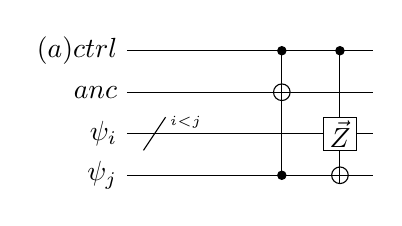
\begin{tikzpicture}[scale=1.000000,x=1pt,y=1pt]
\filldraw[color=white] (0.000000, -7.500000) rectangle (89.000000, 52.500000);
% Drawing wires
% Line 1: ctrl W \text{(a) }ctrl
\draw[color=black] (0.000000,45.000000) -- (89.000000,45.000000);
\draw[color=black] (0.000000,45.000000) node[left] {$\text{(a) }ctrl$};
% Line 2: anc W anc
\draw[color=black] (0.000000,30.000000) -- (89.000000,30.000000);
\draw[color=black] (0.000000,30.000000) node[left] {$anc$};
% Line 3: i W \psi_i
\draw[color=black] (0.000000,15.000000) -- (89.000000,15.000000);
\draw[color=black] (0.000000,15.000000) node[left] {$\psi_i$};
% Line 4: j W \psi_j
\draw[color=black] (0.000000,0.000000) -- (89.000000,0.000000);
\draw[color=black] (0.000000,0.000000) node[left] {$\psi_j$};
% Done with wires; drawing gates
% Line 6: i / ^{i<j}
\draw (6.000000, 9.000000) -- (14.000000, 21.000000);
\draw (12.000000, 18.000000) node[right] {$\scriptstyle{^{i<j}}$};
% Line 7: ctrl anc i j LABEL
% Line 8: ctrl j +anc
\draw (56.000000,45.000000) -- (56.000000,0.000000);
\filldraw (56.000000, 45.000000) circle(1.500000pt);
\filldraw (56.000000, 0.000000) circle(1.500000pt);
\begin{scope}
\draw[fill=white] (56.000000, 30.000000) circle(3.000000pt);
\clip (56.000000, 30.000000) circle(3.000000pt);
\draw (53.000000, 30.000000) -- (59.000000, 30.000000);
\draw (56.000000, 27.000000) -- (56.000000, 33.000000);
\end{scope}
% Line 10: i G $\vec{Z}$ ctrl +j
\draw (77.000000,45.000000) -- (77.000000,0.000000);
\begin{scope}
\draw[fill=white] (77.000000, 15.000000) +(-45.000000:8.485281pt and 8.485281pt) -- +(45.000000:8.485281pt and 8.485281pt) -- +(135.000000:8.485281pt and 8.485281pt) -- +(225.000000:8.485281pt and 8.485281pt) -- cycle;
\clip (77.000000, 15.000000) +(-45.000000:8.485281pt and 8.485281pt) -- +(45.000000:8.485281pt and 8.485281pt) -- +(135.000000:8.485281pt and 8.485281pt) -- +(225.000000:8.485281pt and 8.485281pt) -- cycle;
\draw (77.000000, 15.000000) node {$\vec{Z}$};
\end{scope}
\filldraw (77.000000, 45.000000) circle(1.500000pt);
\begin{scope}
\draw[fill=white] (77.000000, 0.000000) circle(3.000000pt);
\clip (77.000000, 0.000000) circle(3.000000pt);
\draw (74.000000, 0.000000) -- (80.000000, 0.000000);
\draw (77.000000, -3.000000) -- (77.000000, 3.000000);
\end{scope}
% Done with gates; drawing ending labels
% Done with ending labels; drawing cut lines and comments
% Done with comments
\end{tikzpicture}

        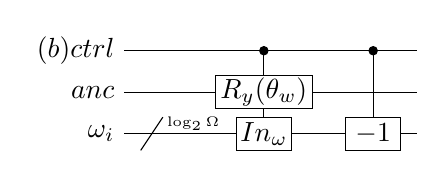
\begin{tikzpicture}[scale=1.000000,x=1pt,y=1pt]
\filldraw[color=white] (0.000000, -7.500000) rectangle (106.000000, 37.500000);
% Drawing wires
% Line 1: ctrl W \text{(b) }ctrl
\draw[color=black] (0.000000,30.000000) -- (106.000000,30.000000);
\draw[color=black] (0.000000,30.000000) node[left] {$\text{(b) }ctrl$};
% Line 2: anc W anc
\draw[color=black] (0.000000,15.000000) -- (106.000000,15.000000);
\draw[color=black] (0.000000,15.000000) node[left] {$anc$};
% Line 3: i W \omega_i
\draw[color=black] (0.000000,0.000000) -- (106.000000,0.000000);
\draw[color=black] (0.000000,0.000000) node[left] {$\omega_i$};
% Done with wires; drawing gates
% Line 5: i / ^{\log_2{\Omega}}
\draw (6.000000, -6.000000) -- (14.000000, 6.000000);
\draw (12.000000, 3.000000) node[right] {$\scriptstyle{^{\log_2{\Omega}}}$};
% Line 6: ctrl anc i LABEL width=-5
% Line 8: anc G:width=35 $R_y(\theta_w)$ i G:width=20 $In_\omega$ ctrl
\draw (50.500000,30.000000) -- (50.500000,0.000000);
\begin{scope}
\draw[fill=white] (50.500000, 15.000000) +(-45.000000:24.748737pt and 8.485281pt) -- +(45.000000:24.748737pt and 8.485281pt) -- +(135.000000:24.748737pt and 8.485281pt) -- +(225.000000:24.748737pt and 8.485281pt) -- cycle;
\clip (50.500000, 15.000000) +(-45.000000:24.748737pt and 8.485281pt) -- +(45.000000:24.748737pt and 8.485281pt) -- +(135.000000:24.748737pt and 8.485281pt) -- +(225.000000:24.748737pt and 8.485281pt) -- cycle;
\draw (50.500000, 15.000000) node {$R_y(\theta_w)$};
\end{scope}
\begin{scope}
\draw[fill=white] (50.500000, -0.000000) +(-45.000000:14.142136pt and 8.485281pt) -- +(45.000000:14.142136pt and 8.485281pt) -- +(135.000000:14.142136pt and 8.485281pt) -- +(225.000000:14.142136pt and 8.485281pt) -- cycle;
\clip (50.500000, -0.000000) +(-45.000000:14.142136pt and 8.485281pt) -- +(45.000000:14.142136pt and 8.485281pt) -- +(135.000000:14.142136pt and 8.485281pt) -- +(225.000000:14.142136pt and 8.485281pt) -- cycle;
\draw (50.500000, -0.000000) node {$In_\omega$};
\end{scope}
\filldraw (50.500000, 30.000000) circle(1.500000pt);
% Line 9: i G width=20 $-1$ ctrl
\draw (90.000000,30.000000) -- (90.000000,0.000000);
\begin{scope}
\draw[fill=white] (90.000000, -0.000000) +(-45.000000:14.142136pt and 8.485281pt) -- +(45.000000:14.142136pt and 8.485281pt) -- +(135.000000:14.142136pt and 8.485281pt) -- +(225.000000:14.142136pt and 8.485281pt) -- cycle;
\clip (90.000000, -0.000000) +(-45.000000:14.142136pt and 8.485281pt) -- +(45.000000:14.142136pt and 8.485281pt) -- +(135.000000:14.142136pt and 8.485281pt) -- +(225.000000:14.142136pt and 8.485281pt) -- cycle;
\draw (90.000000, -0.000000) node {$-1$};
\end{scope}
\filldraw (90.000000, 30.000000) circle(1.500000pt);
% Done with gates; drawing ending labels
% Done with ending labels; drawing cut lines and comments
% Done with comments
\end{tikzpicture}

    }
    \caption{
        \textbf{Fermionic Ladder Operator Block-Encodings}
        In (a), a block-encoding for the fermionic creation operator acting on the $j^\text{th}$ mode is given.
        In (b), a block-encoding for the fermionic annihilation operator acting on the $j^\text{th}$ mode is given.
        For a creation (annihilation) operator, the branch of the wavefunction will be flipped outside of the encoded subspace if the mode is occupied (unoccupied).
        The state is updated by applying Pauli $Z$ gates to the preceeding fermionic modes which result in the output state having the appropriate sign based on $p(\psi)$.
        Then a Pauli $X$ gate is applied to flip the occupation of the $j^\text{th}$ mode.
    }
    \label{fig:fermionic-be}
\end{figure}


An implementation for $U_{b^\dagger_j}$ is given in subfigure \ref{fig:fermionic-be}a.
The initial Toffoli gate flips the ancilla qubit to indicate that the state has been zeroed-out when the control qubit is on ($\ket{1}$) and the fermionic mode is occupied ($\ket{1}$).
The sign of the output state corresponding to $p(\psi)$ can be applied appropriately using a series of controlled Pauli $Z$ operators applied to each of the fermionic modes with index $i < j$: $\vec{Z}_i$.
The occupation of the fermionic mode on which the ladder operator acts is updated using a controlled Pauli $X$ operator: $X_j$.

A block-encoding for the fermionic annihilation operator, $U_{b_j}$, can be constructed similarly to $U_{b^\dagger_j}$ and is shown in subfigue \ref{fig:fermionic-be}b.
The fermionic creation operator ($b^\dagger$) only acts nontrivially when the mode it acts upon is \textit{unoccupied}.
Inversely, the fermionic annihilation operator ($b$) will only act nontrivially if the mode it acts upon is \textit{occupied}.
Therefore, the block-encoding ancilla is flipped outside of the encoded subspace if the control qubit is on ($\ket{1}$) and the fermionic mode is unoccupied ($\ket{0}$).

As noted in Appendix \ref{sec:elbows}, each Toffoli gate can be implemented with four T gates using one clean ancilla.
These block-encodings have an optimal rescaling factor ($\lambda = 1$), require one block-encoding ancilla and one clean ancillae, and use four T gates.

\subsection{Products of Fermionic Ladder Operators}

As discussed in subsection \ref{subsec:be-products}, a block-encoding for a product of operators can be constructed using a product of the unitaries that block-encode each operator.
In this subsection, we construct block-encodings for a product of fermionic ladder operators that use fewer quantum resources than are required by this naive strategy.

\begin{figure}[h]
    \mbox{
        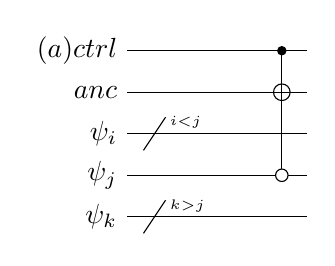
\begin{tikzpicture}[scale=1.000000,x=1pt,y=1pt]
\filldraw[color=white] (0.000000, -7.500000) rectangle (65.000000, 67.500000);
% Drawing wires
% Line 1: ctrl W \text{(a) }ctrl
\draw[color=black] (0.000000,60.000000) -- (65.000000,60.000000);
\draw[color=black] (0.000000,60.000000) node[left] {$\text{(a) }ctrl$};
% Line 2: anc W anc
\draw[color=black] (0.000000,45.000000) -- (65.000000,45.000000);
\draw[color=black] (0.000000,45.000000) node[left] {$anc$};
% Line 3: i W \psi_i
\draw[color=black] (0.000000,30.000000) -- (65.000000,30.000000);
\draw[color=black] (0.000000,30.000000) node[left] {$\psi_i$};
% Line 4: j W \psi_j
\draw[color=black] (0.000000,15.000000) -- (65.000000,15.000000);
\draw[color=black] (0.000000,15.000000) node[left] {$\psi_j$};
% Line 5: k W \psi_k
\draw[color=black] (0.000000,0.000000) -- (65.000000,0.000000);
\draw[color=black] (0.000000,0.000000) node[left] {$\psi_k$};
% Done with wires; drawing gates
% Line 7: i / ^{i<j}
\draw (6.000000, 24.000000) -- (14.000000, 36.000000);
\draw (12.000000, 33.000000) node[right] {$\scriptstyle{^{i<j}}$};
% Line 8: k / ^{k>j}
\draw (6.000000, -6.000000) -- (14.000000, 6.000000);
\draw (12.000000, 3.000000) node[right] {$\scriptstyle{^{k>j}}$};
% Line 9: ctrl anc i j k LABEL
% Line 10: -j +anc ctrl
\draw (56.000000,60.000000) -- (56.000000,15.000000);
\draw[fill=white] (56.000000, 15.000000) circle(2.250000pt);
\begin{scope}
\draw[fill=white] (56.000000, 45.000000) circle(3.000000pt);
\clip (56.000000, 45.000000) circle(3.000000pt);
\draw (53.000000, 45.000000) -- (59.000000, 45.000000);
\draw (56.000000, 42.000000) -- (56.000000, 48.000000);
\end{scope}
\filldraw (56.000000, 60.000000) circle(1.500000pt);
% Done with gates; drawing ending labels
% Done with ending labels; drawing cut lines and comments
% Done with comments
\end{tikzpicture}

        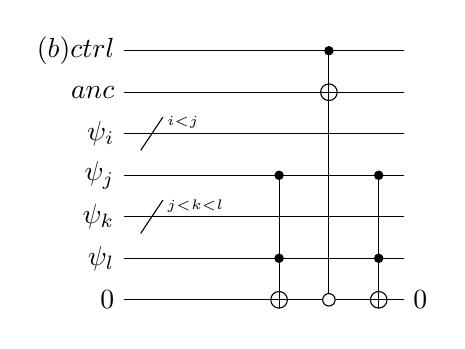
\begin{tikzpicture}[scale=1.000000,x=1pt,y=1pt]
\filldraw[color=white] (0.000000, -7.500000) rectangle (101.000000, 97.500000);
% Drawing wires
% Line 1: ctrl W \text{(b) }ctrl
\draw[color=black] (0.000000,90.000000) -- (101.000000,90.000000);
\draw[color=black] (0.000000,90.000000) node[left] {$\text{(b) }ctrl$};
% Line 2: anc W anc
\draw[color=black] (0.000000,75.000000) -- (101.000000,75.000000);
\draw[color=black] (0.000000,75.000000) node[left] {$anc$};
% Line 3: i W \psi_i
\draw[color=black] (0.000000,60.000000) -- (101.000000,60.000000);
\draw[color=black] (0.000000,60.000000) node[left] {$\psi_i$};
% Line 4: j W \psi_j
\draw[color=black] (0.000000,45.000000) -- (101.000000,45.000000);
\draw[color=black] (0.000000,45.000000) node[left] {$\psi_j$};
% Line 5: k W \psi_k
\draw[color=black] (0.000000,30.000000) -- (101.000000,30.000000);
\draw[color=black] (0.000000,30.000000) node[left] {$\psi_k$};
% Line 6: l W \psi_l
\draw[color=black] (0.000000,15.000000) -- (101.000000,15.000000);
\draw[color=black] (0.000000,15.000000) node[left] {$\psi_l$};
% Line 7: clean0 W 0 0
\draw[color=black] (0.000000,0.000000) -- (101.000000,0.000000);
\draw[color=black] (0.000000,0.000000) node[left] {$0$};
% Done with wires; drawing gates
% Line 9: i / ^{i<j}
\draw (6.000000, 54.000000) -- (14.000000, 66.000000);
\draw (12.000000, 63.000000) node[right] {$\scriptstyle{^{i<j}}$};
% Line 10: k / ^{j<k<l}
\draw (6.000000, 24.000000) -- (14.000000, 36.000000);
\draw (12.000000, 33.000000) node[right] {$\scriptstyle{^{j<k<l}}$};
% Line 11: ctrl anc i j k l clean0 LABEL
% Line 12: j l +clean0
\draw (56.000000,45.000000) -- (56.000000,0.000000);
\filldraw (56.000000, 45.000000) circle(1.500000pt);
\filldraw (56.000000, 15.000000) circle(1.500000pt);
\begin{scope}
\draw[fill=white] (56.000000, 0.000000) circle(3.000000pt);
\clip (56.000000, 0.000000) circle(3.000000pt);
\draw (53.000000, 0.000000) -- (59.000000, 0.000000);
\draw (56.000000, -3.000000) -- (56.000000, 3.000000);
\end{scope}
% Line 13: -clean0 ctrl +anc
\draw (74.000000,90.000000) -- (74.000000,0.000000);
\draw[fill=white] (74.000000, 0.000000) circle(2.250000pt);
\filldraw (74.000000, 90.000000) circle(1.500000pt);
\begin{scope}
\draw[fill=white] (74.000000, 75.000000) circle(3.000000pt);
\clip (74.000000, 75.000000) circle(3.000000pt);
\draw (71.000000, 75.000000) -- (77.000000, 75.000000);
\draw (74.000000, 72.000000) -- (74.000000, 78.000000);
\end{scope}
% Line 14: j l +clean0
\draw (92.000000,45.000000) -- (92.000000,0.000000);
\filldraw (92.000000, 45.000000) circle(1.500000pt);
\filldraw (92.000000, 15.000000) circle(1.500000pt);
\begin{scope}
\draw[fill=white] (92.000000, 0.000000) circle(3.000000pt);
\clip (92.000000, 0.000000) circle(3.000000pt);
\draw (89.000000, 0.000000) -- (95.000000, 0.000000);
\draw (92.000000, -3.000000) -- (92.000000, 3.000000);
\end{scope}
% Done with gates; drawing ending labels
\draw[color=black] (101.000000,0.000000) node[right] {$0$};
% Done with ending labels; drawing cut lines and comments
% Done with comments
\end{tikzpicture}

    }
    \mbox{
        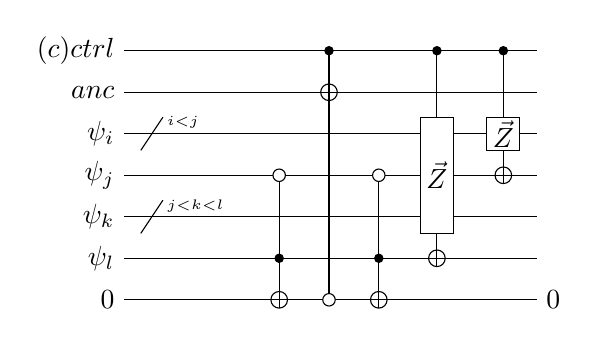
\begin{tikzpicture}[scale=1.000000,x=1pt,y=1pt]
\filldraw[color=white] (0.000000, -7.500000) rectangle (149.000000, 97.500000);
% Drawing wires
% Line 1: ctrl W \text{(c) }ctrl
\draw[color=black] (0.000000,90.000000) -- (149.000000,90.000000);
\draw[color=black] (0.000000,90.000000) node[left] {$\text{(c) }ctrl$};
% Line 2: anc W anc
\draw[color=black] (0.000000,75.000000) -- (149.000000,75.000000);
\draw[color=black] (0.000000,75.000000) node[left] {$anc$};
% Line 3: i W \psi_i
\draw[color=black] (0.000000,60.000000) -- (149.000000,60.000000);
\draw[color=black] (0.000000,60.000000) node[left] {$\psi_i$};
% Line 4: j W \psi_j
\draw[color=black] (0.000000,45.000000) -- (149.000000,45.000000);
\draw[color=black] (0.000000,45.000000) node[left] {$\psi_j$};
% Line 5: k W \psi_k
\draw[color=black] (0.000000,30.000000) -- (149.000000,30.000000);
\draw[color=black] (0.000000,30.000000) node[left] {$\psi_k$};
% Line 6: l W \psi_l
\draw[color=black] (0.000000,15.000000) -- (149.000000,15.000000);
\draw[color=black] (0.000000,15.000000) node[left] {$\psi_l$};
% Line 7: clean0 W 0 0
\draw[color=black] (0.000000,0.000000) -- (149.000000,0.000000);
\draw[color=black] (0.000000,0.000000) node[left] {$0$};
% Done with wires; drawing gates
% Line 9: i / ^{i<j}
\draw (6.000000, 54.000000) -- (14.000000, 66.000000);
\draw (12.000000, 63.000000) node[right] {$\scriptstyle{^{i<j}}$};
% Line 10: k / ^{j<k<l}
\draw (6.000000, 24.000000) -- (14.000000, 36.000000);
\draw (12.000000, 33.000000) node[right] {$\scriptstyle{^{j<k<l}}$};
% Line 11: ctrl anc i j k l clean0 LABEL
% Line 13: -j l +clean0
\draw (56.000000,45.000000) -- (56.000000,0.000000);
\draw[fill=white] (56.000000, 45.000000) circle(2.250000pt);
\filldraw (56.000000, 15.000000) circle(1.500000pt);
\begin{scope}
\draw[fill=white] (56.000000, 0.000000) circle(3.000000pt);
\clip (56.000000, 0.000000) circle(3.000000pt);
\draw (53.000000, 0.000000) -- (59.000000, 0.000000);
\draw (56.000000, -3.000000) -- (56.000000, 3.000000);
\end{scope}
% Line 14: ctrl +anc -clean0
\draw (74.000000,90.000000) -- (74.000000,0.000000);
\filldraw (74.000000, 90.000000) circle(1.500000pt);
\begin{scope}
\draw[fill=white] (74.000000, 75.000000) circle(3.000000pt);
\clip (74.000000, 75.000000) circle(3.000000pt);
\draw (71.000000, 75.000000) -- (77.000000, 75.000000);
\draw (74.000000, 72.000000) -- (74.000000, 78.000000);
\end{scope}
\draw[fill=white] (74.000000, 0.000000) circle(2.250000pt);
% Line 15: -j l +clean0
\draw (92.000000,45.000000) -- (92.000000,0.000000);
\draw[fill=white] (92.000000, 45.000000) circle(2.250000pt);
\filldraw (92.000000, 15.000000) circle(1.500000pt);
\begin{scope}
\draw[fill=white] (92.000000, 0.000000) circle(3.000000pt);
\clip (92.000000, 0.000000) circle(3.000000pt);
\draw (89.000000, 0.000000) -- (95.000000, 0.000000);
\draw (92.000000, -3.000000) -- (92.000000, 3.000000);
\end{scope}
% Line 17: i j k G $\vec{Z}$ +l ctrl
\draw (113.000000,90.000000) -- (113.000000,15.000000);
\begin{scope}
\draw[fill=white] (113.000000, 45.000000) +(-45.000000:8.485281pt and 29.698485pt) -- +(45.000000:8.485281pt and 29.698485pt) -- +(135.000000:8.485281pt and 29.698485pt) -- +(225.000000:8.485281pt and 29.698485pt) -- cycle;
\clip (113.000000, 45.000000) +(-45.000000:8.485281pt and 29.698485pt) -- +(45.000000:8.485281pt and 29.698485pt) -- +(135.000000:8.485281pt and 29.698485pt) -- +(225.000000:8.485281pt and 29.698485pt) -- cycle;
\draw (113.000000, 45.000000) node {$\vec{Z}$};
\end{scope}
\begin{scope}
\draw[fill=white] (113.000000, 15.000000) circle(3.000000pt);
\clip (113.000000, 15.000000) circle(3.000000pt);
\draw (110.000000, 15.000000) -- (116.000000, 15.000000);
\draw (113.000000, 12.000000) -- (113.000000, 18.000000);
\end{scope}
\filldraw (113.000000, 90.000000) circle(1.500000pt);
% Line 18: i G $\vec{Z}$ +j ctrl
\draw (137.000000,90.000000) -- (137.000000,45.000000);
\begin{scope}
\draw[fill=white] (137.000000, 60.000000) +(-45.000000:8.485281pt and 8.485281pt) -- +(45.000000:8.485281pt and 8.485281pt) -- +(135.000000:8.485281pt and 8.485281pt) -- +(225.000000:8.485281pt and 8.485281pt) -- cycle;
\clip (137.000000, 60.000000) +(-45.000000:8.485281pt and 8.485281pt) -- +(45.000000:8.485281pt and 8.485281pt) -- +(135.000000:8.485281pt and 8.485281pt) -- +(225.000000:8.485281pt and 8.485281pt) -- cycle;
\draw (137.000000, 60.000000) node {$\vec{Z}$};
\end{scope}
\begin{scope}
\draw[fill=white] (137.000000, 45.000000) circle(3.000000pt);
\clip (137.000000, 45.000000) circle(3.000000pt);
\draw (134.000000, 45.000000) -- (140.000000, 45.000000);
\draw (137.000000, 42.000000) -- (137.000000, 48.000000);
\end{scope}
\filldraw (137.000000, 90.000000) circle(1.500000pt);
% Done with gates; drawing ending labels
\draw[color=black] (149.000000,0.000000) node[right] {$0$};
% Done with ending labels; drawing cut lines and comments
% Done with comments
\end{tikzpicture}

    }
    \mbox{
        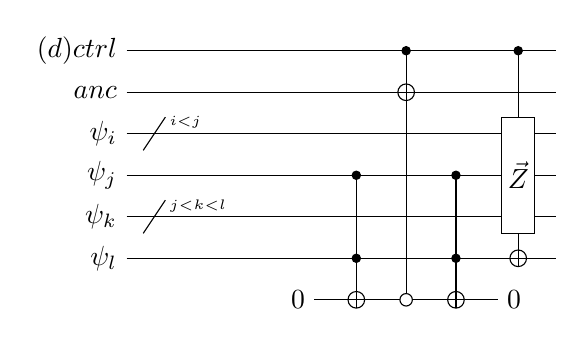
\begin{tikzpicture}[scale=1.000000,x=1pt,y=1pt]
\filldraw[color=white] (0.000000, -7.500000) rectangle (155.000000, 97.500000);
% Drawing wires
% Line 1: ctrl W \text{(d) }ctrl
\draw[color=black] (0.000000,90.000000) -- (155.000000,90.000000);
\draw[color=black] (0.000000,90.000000) node[left] {$\text{(d) }ctrl$};
% Line 2: anc W anc
\draw[color=black] (0.000000,75.000000) -- (155.000000,75.000000);
\draw[color=black] (0.000000,75.000000) node[left] {$anc$};
% Line 3: i W \psi_i
\draw[color=black] (0.000000,60.000000) -- (155.000000,60.000000);
\draw[color=black] (0.000000,60.000000) node[left] {$\psi_i$};
% Line 4: j W \psi_j
\draw[color=black] (0.000000,45.000000) -- (155.000000,45.000000);
\draw[color=black] (0.000000,45.000000) node[left] {$\psi_j$};
% Line 5: k W \psi_k
\draw[color=black] (0.000000,30.000000) -- (155.000000,30.000000);
\draw[color=black] (0.000000,30.000000) node[left] {$\psi_k$};
% Line 6: l W \psi_l
\draw[color=black] (0.000000,15.000000) -- (155.000000,15.000000);
\draw[color=black] (0.000000,15.000000) node[left] {$\psi_l$};
% Line 7: clean0 W 0 0
\draw[color=black] (60.500000,0.000000) -- (141.500000,0.000000);
% Done with wires; drawing gates
% Line 9: i / ^{i<j}
\draw (6.000000, 54.000000) -- (14.000000, 66.000000);
\draw (12.000000, 63.000000) node[right] {$\scriptstyle{^{i<j}}$};
% Line 10: k / ^{j<k<l}
\draw (6.000000, 24.000000) -- (14.000000, 36.000000);
\draw (12.000000, 33.000000) node[right] {$\scriptstyle{^{j<k<l}}$};
% Line 11: ctrl anc i j k l clean0 LABEL
% Line 13: clean0 START
\draw[color=black] (68.000000,0.000000) node[fill=white,left,minimum height=15.000000pt,minimum width=15.000000pt,inner sep=0pt] {\phantom{$0$}};
\draw[color=black] (68.000000,0.000000) node[left] {$0$};
% Line 14: j l +clean0
\draw (83.000000,45.000000) -- (83.000000,0.000000);
\filldraw (83.000000, 45.000000) circle(1.500000pt);
\filldraw (83.000000, 15.000000) circle(1.500000pt);
\begin{scope}
\draw[fill=white] (83.000000, 0.000000) circle(3.000000pt);
\clip (83.000000, 0.000000) circle(3.000000pt);
\draw (80.000000, 0.000000) -- (86.000000, 0.000000);
\draw (83.000000, -3.000000) -- (83.000000, 3.000000);
\end{scope}
% Line 15: ctrl +anc -clean0
\draw (101.000000,90.000000) -- (101.000000,0.000000);
\filldraw (101.000000, 90.000000) circle(1.500000pt);
\begin{scope}
\draw[fill=white] (101.000000, 75.000000) circle(3.000000pt);
\clip (101.000000, 75.000000) circle(3.000000pt);
\draw (98.000000, 75.000000) -- (104.000000, 75.000000);
\draw (101.000000, 72.000000) -- (101.000000, 78.000000);
\end{scope}
\draw[fill=white] (101.000000, 0.000000) circle(2.250000pt);
% Line 16: j l +clean0
\draw (119.000000,45.000000) -- (119.000000,0.000000);
\filldraw (119.000000, 45.000000) circle(1.500000pt);
\filldraw (119.000000, 15.000000) circle(1.500000pt);
\begin{scope}
\draw[fill=white] (119.000000, 0.000000) circle(3.000000pt);
\clip (119.000000, 0.000000) circle(3.000000pt);
\draw (116.000000, 0.000000) -- (122.000000, 0.000000);
\draw (119.000000, -3.000000) -- (119.000000, 3.000000);
\end{scope}
% Line 17: clean0 END
\draw[color=black] (134.000000,0.000000) node[fill=white,right,minimum height=15.000000pt,minimum width=15.000000pt,inner sep=0pt] {\phantom{$0$}};
\draw[color=black] (134.000000,0.000000) node[right] {$0$};
% Line 19: i j k G $\vec{Z}$ +l ctrl
\draw (141.500000,90.000000) -- (141.500000,15.000000);
\begin{scope}
\draw[fill=white] (141.500000, 45.000000) +(-45.000000:8.485281pt and 29.698485pt) -- +(45.000000:8.485281pt and 29.698485pt) -- +(135.000000:8.485281pt and 29.698485pt) -- +(225.000000:8.485281pt and 29.698485pt) -- cycle;
\clip (141.500000, 45.000000) +(-45.000000:8.485281pt and 29.698485pt) -- +(45.000000:8.485281pt and 29.698485pt) -- +(135.000000:8.485281pt and 29.698485pt) -- +(225.000000:8.485281pt and 29.698485pt) -- cycle;
\draw (141.500000, 45.000000) node {$\vec{Z}$};
\end{scope}
\begin{scope}
\draw[fill=white] (141.500000, 15.000000) circle(3.000000pt);
\clip (141.500000, 15.000000) circle(3.000000pt);
\draw (138.500000, 15.000000) -- (144.500000, 15.000000);
\draw (141.500000, 12.000000) -- (141.500000, 18.000000);
\end{scope}
\filldraw (141.500000, 90.000000) circle(1.500000pt);
% Done with gates; drawing ending labels
% Done with ending labels; drawing cut lines and comments
% Done with comments
\end{tikzpicture}

    }
    \caption{
        \textbf{Block-Encoding Products of Fermionic Ladder Operators}
        In (a), a block-encoding for the fermionic number operator acting on the $i^\text{th}$ mode ($b_i^\dagger b_i$) is given.
        In (b), a block-encoding for the product of two fermionic number operators acting on the $i^\text{th}$ and $j^\text{th}$ modes ($b_i^\dagger b_i b_j^\dagger b_j$) is given.
        In (c), a block-encoding for the operator $b_j^\dagger b_l$ with $i \neq l$ is given.
        In (d), a block-encoding for the operator $b_j^\dagger b_j b_l$ with $i \neq l$ is given.
    }
    \label{fig:fermionic-products-be}
\end{figure}

Consider the action of the fermionic number operator ($b_i^\dagger b_i$):
\begin{equation}
    \begin{split}
        b_i^\dagger b_i \ket{\psi_{b_i}} = \begin{cases} 
            \ket{1} & \text{when $\ket{\psi_{b_i}}$ is $\ket{1}$} \\
            0 & \text{when $\ket{\psi_{b_i}}$ is $\ket{0}$} \\
                                        \end{cases}
    \end{split}
\end{equation}
If the $i^\text{th}$ mode is unoccupied, the state will be zeroed-out.
If the $i^\text{th}$ mode is occupied, then the state is left unchanged.

This action can be encoded using the circuit shown in subfigure \ref{fig:fermionic-products-be}a.
The Toffoli gate flips the block-encoding ancilla outside of the encoded subspace if the control is on and the $i^\text{th}$ mode is unoccupied.
Otherwise, the state of the system and the block-encoding ancilla are left unchanged.

Block-encoding this operator as the product of the block-encodings for $b_i$ and $b_i^\dagger$ would require two block-encoding ancillae and use $8$ T gates.
Meanwhile, this construction has an optimal rescaling factor ($\lambda = 1$), requires one block-encoding ancilla and one clean ancilla, and uses four T gates.
For circuit diagrams shown throughout this section, an $N$-controlled Toffoli gate acting on a clean ancilla is intended to denote a ``left-elbow'' as described in more detail in Appendix \ref{sec:elbows}.
Likewise, $N$-controlled Toffoli gates that result in a clean ancilla being returned to the zero-state denote ``right-elbows''.

A block-encoding circuit for the operator $b_j^\dagger b_l$ is given in subfigure \ref{fig:fermionic-products-be}c.
For this operator, we can infer that the state will be zeroed-out \textit{unless} both the $j^\text{th}$ mode is unoccupied and the $l^\text{th}$ mode is occupied.
If the control qubit is on and these two conditions are not both true, then the block-encoding ancilla is flipped outside of the encoded subspace.
The state of the system is updated based on the two operators in the order in which they would act upon the quantum state: $\vec{Z}X_l$ ($b_l$) then $\vec{Z}X_j$ ($b_j^\dagger$).
This block-encoding circuit has an optimal rescaling factor ($\lambda = 1$), requires one block-encoding ancilla and two clean ancillae, and uses $8$ T gates.


This construction can be generalized to an arbitrary product of ladder operators.
Let $B$ represent the number of active modes in an operator.
We define the number of ``active modes" as the number of unique modes upon which an operator is applied nontrivially.
For example, the operator $b_i b_j^\dagger b_k b_l^\dagger b_l$ has $4$ active modes: $i, j, k, l$.
Each active mode will contribute a new control condition on the state of the corresponding mode.
Therefore, a block-encoding circuit for a general product of fermionic ladder operators with $B$ active modes will have an optimal rescaling factor ($\lambda = 1$), require one block-encoding ancilla and $B$ clean ancillae, and use $4B$ T gates.


\subsection{Linear Combinations of Fermionic Ladder Operators}

As discussed in subsection \ref{subsec:lco}, a block-encoding for a linear combination of operators can be constructed using the LCO framework.
In this subsection, we show how to construct block-encodings of linear combinations of products of fermionic ladder operators that use fewer quantum resources than are required by an LCO construction.
In particular, we give a generalized construction for a product of fermionic ladder operators plus its hermitian conjugate, however, we note that the strategies we present here are not restricted to a linear combination of hermitian conjugates.

\begin{figure*}
    \mbox{
        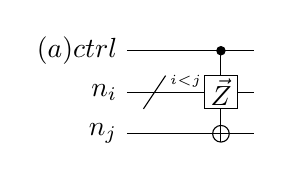
\begin{tikzpicture}[scale=1.000000,x=1pt,y=1pt]
\filldraw[color=white] (0.000000, -7.500000) rectangle (46.000000, 37.500000);
% Drawing wires
% Line 1: a W \text{(a) }ctrl
\draw[color=black] (0.000000,30.000000) -- (46.000000,30.000000);
\draw[color=black] (0.000000,30.000000) node[left] {$\text{(a) }ctrl$};
% Line 2: b W n_i
\draw[color=black] (0.000000,15.000000) -- (46.000000,15.000000);
\draw[color=black] (0.000000,15.000000) node[left] {$n_i$};
% Line 3: c W n_j
\draw[color=black] (0.000000,0.000000) -- (46.000000,0.000000);
\draw[color=black] (0.000000,0.000000) node[left] {$n_j$};
% Done with wires; drawing gates
% Line 5: b / ^{i<j}
\draw (6.000000, 9.000000) -- (14.000000, 21.000000);
\draw (12.000000, 18.000000) node[right] {$\scriptstyle{^{i<j}}$};
% Line 6: a b c LABEL width=-10
% Line 7: b G $\vec{Z}$ a +c
\draw (34.000000,30.000000) -- (34.000000,0.000000);
\begin{scope}
\draw[fill=white] (34.000000, 15.000000) +(-45.000000:8.485281pt and 8.485281pt) -- +(45.000000:8.485281pt and 8.485281pt) -- +(135.000000:8.485281pt and 8.485281pt) -- +(225.000000:8.485281pt and 8.485281pt) -- cycle;
\clip (34.000000, 15.000000) +(-45.000000:8.485281pt and 8.485281pt) -- +(45.000000:8.485281pt and 8.485281pt) -- +(135.000000:8.485281pt and 8.485281pt) -- +(225.000000:8.485281pt and 8.485281pt) -- cycle;
\draw (34.000000, 15.000000) node {$\vec{Z}$};
\end{scope}
\filldraw (34.000000, 30.000000) circle(1.500000pt);
\begin{scope}
\draw[fill=white] (34.000000, 0.000000) circle(3.000000pt);
\clip (34.000000, 0.000000) circle(3.000000pt);
\draw (31.000000, 0.000000) -- (37.000000, 0.000000);
\draw (34.000000, -3.000000) -- (34.000000, 3.000000);
\end{scope}
% Done with gates; drawing ending labels
% Done with ending labels; drawing cut lines and comments
% Done with comments
\end{tikzpicture}

        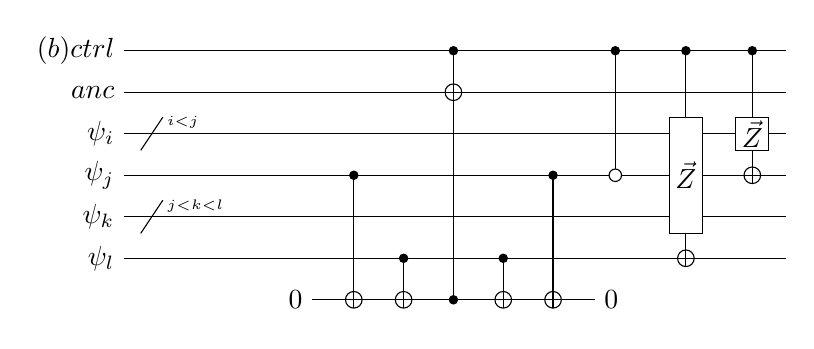
\begin{tikzpicture}[scale=1.000000,x=1pt,y=1pt]
\filldraw[color=white] (0.000000, -7.500000) rectangle (239.000000, 97.500000);
% Drawing wires
% Line 1: c W \text{(b) }ctrl
\draw[color=black] (0.000000,90.000000) -- (239.000000,90.000000);
\draw[color=black] (0.000000,90.000000) node[left] {$\text{(b) }ctrl$};
% Line 2: a W anc
\draw[color=black] (0.000000,75.000000) -- (239.000000,75.000000);
\draw[color=black] (0.000000,75.000000) node[left] {$anc$};
% Line 3: i W \psi_i
\draw[color=black] (0.000000,60.000000) -- (239.000000,60.000000);
\draw[color=black] (0.000000,60.000000) node[left] {$\psi_i$};
% Line 4: j W \psi_j
\draw[color=black] (0.000000,45.000000) -- (239.000000,45.000000);
\draw[color=black] (0.000000,45.000000) node[left] {$\psi_j$};
% Line 5: k W \psi_k
\draw[color=black] (0.000000,30.000000) -- (239.000000,30.000000);
\draw[color=black] (0.000000,30.000000) node[left] {$\psi_k$};
% Line 6: l W \psi_l
\draw[color=black] (0.000000,15.000000) -- (239.000000,15.000000);
\draw[color=black] (0.000000,15.000000) node[left] {$\psi_l$};
% Line 7: c0 W 0 0
\draw[color=black] (60.500000,0.000000) -- (177.500000,0.000000);
% Done with wires; drawing gates
% Line 9: i / ^{i<j}
\draw (6.000000, 54.000000) -- (14.000000, 66.000000);
\draw (12.000000, 63.000000) node[right] {$\scriptstyle{^{i<j}}$};
% Line 10: k / ^{j<k<l}
\draw (6.000000, 24.000000) -- (14.000000, 36.000000);
\draw (12.000000, 33.000000) node[right] {$\scriptstyle{^{j<k<l}}$};
% Line 11: c a i j k l c0 LABEL
% Line 12: c0 START
\draw[color=black] (68.000000,0.000000) node[fill=white,left,minimum height=15.000000pt,minimum width=15.000000pt,inner sep=0pt] {\phantom{$0$}};
\draw[color=black] (68.000000,0.000000) node[left] {$0$};
% Line 13: j +c0
\draw (83.000000,45.000000) -- (83.000000,0.000000);
\filldraw (83.000000, 45.000000) circle(1.500000pt);
\begin{scope}
\draw[fill=white] (83.000000, 0.000000) circle(3.000000pt);
\clip (83.000000, 0.000000) circle(3.000000pt);
\draw (80.000000, 0.000000) -- (86.000000, 0.000000);
\draw (83.000000, -3.000000) -- (83.000000, 3.000000);
\end{scope}
% Line 14: l +c0
\draw (101.000000,15.000000) -- (101.000000,0.000000);
\filldraw (101.000000, 15.000000) circle(1.500000pt);
\begin{scope}
\draw[fill=white] (101.000000, 0.000000) circle(3.000000pt);
\clip (101.000000, 0.000000) circle(3.000000pt);
\draw (98.000000, 0.000000) -- (104.000000, 0.000000);
\draw (101.000000, -3.000000) -- (101.000000, 3.000000);
\end{scope}
% Line 15: c c0 +a
\draw (119.000000,90.000000) -- (119.000000,0.000000);
\filldraw (119.000000, 90.000000) circle(1.500000pt);
\filldraw (119.000000, 0.000000) circle(1.500000pt);
\begin{scope}
\draw[fill=white] (119.000000, 75.000000) circle(3.000000pt);
\clip (119.000000, 75.000000) circle(3.000000pt);
\draw (116.000000, 75.000000) -- (122.000000, 75.000000);
\draw (119.000000, 72.000000) -- (119.000000, 78.000000);
\end{scope}
% Line 16: l +c0
\draw (137.000000,15.000000) -- (137.000000,0.000000);
\filldraw (137.000000, 15.000000) circle(1.500000pt);
\begin{scope}
\draw[fill=white] (137.000000, 0.000000) circle(3.000000pt);
\clip (137.000000, 0.000000) circle(3.000000pt);
\draw (134.000000, 0.000000) -- (140.000000, 0.000000);
\draw (137.000000, -3.000000) -- (137.000000, 3.000000);
\end{scope}
% Line 17: j +c0
\draw (155.000000,45.000000) -- (155.000000,0.000000);
\filldraw (155.000000, 45.000000) circle(1.500000pt);
\begin{scope}
\draw[fill=white] (155.000000, 0.000000) circle(3.000000pt);
\clip (155.000000, 0.000000) circle(3.000000pt);
\draw (152.000000, 0.000000) -- (158.000000, 0.000000);
\draw (155.000000, -3.000000) -- (155.000000, 3.000000);
\end{scope}
% Line 18: c0 END
\draw[color=black] (170.000000,0.000000) node[fill=white,right,minimum height=15.000000pt,minimum width=15.000000pt,inner sep=0pt] {\phantom{$0$}};
\draw[color=black] (170.000000,0.000000) node[right] {$0$};
% Line 19: c -j
\draw (177.500000,90.000000) -- (177.500000,45.000000);
\filldraw (177.500000, 90.000000) circle(1.500000pt);
\draw[fill=white] (177.500000, 45.000000) circle(2.250000pt);
% Line 21: i j k G $\vec{Z}$ c +l
\draw (203.000000,90.000000) -- (203.000000,15.000000);
\begin{scope}
\draw[fill=white] (203.000000, 45.000000) +(-45.000000:8.485281pt and 29.698485pt) -- +(45.000000:8.485281pt and 29.698485pt) -- +(135.000000:8.485281pt and 29.698485pt) -- +(225.000000:8.485281pt and 29.698485pt) -- cycle;
\clip (203.000000, 45.000000) +(-45.000000:8.485281pt and 29.698485pt) -- +(45.000000:8.485281pt and 29.698485pt) -- +(135.000000:8.485281pt and 29.698485pt) -- +(225.000000:8.485281pt and 29.698485pt) -- cycle;
\draw (203.000000, 45.000000) node {$\vec{Z}$};
\end{scope}
\filldraw (203.000000, 90.000000) circle(1.500000pt);
\begin{scope}
\draw[fill=white] (203.000000, 15.000000) circle(3.000000pt);
\clip (203.000000, 15.000000) circle(3.000000pt);
\draw (200.000000, 15.000000) -- (206.000000, 15.000000);
\draw (203.000000, 12.000000) -- (203.000000, 18.000000);
\end{scope}
% Line 22: i G $\vec{Z}$ c +j
\draw (227.000000,90.000000) -- (227.000000,45.000000);
\begin{scope}
\draw[fill=white] (227.000000, 60.000000) +(-45.000000:8.485281pt and 8.485281pt) -- +(45.000000:8.485281pt and 8.485281pt) -- +(135.000000:8.485281pt and 8.485281pt) -- +(225.000000:8.485281pt and 8.485281pt) -- cycle;
\clip (227.000000, 60.000000) +(-45.000000:8.485281pt and 8.485281pt) -- +(45.000000:8.485281pt and 8.485281pt) -- +(135.000000:8.485281pt and 8.485281pt) -- +(225.000000:8.485281pt and 8.485281pt) -- cycle;
\draw (227.000000, 60.000000) node {$\vec{Z}$};
\end{scope}
\filldraw (227.000000, 90.000000) circle(1.500000pt);
\begin{scope}
\draw[fill=white] (227.000000, 45.000000) circle(3.000000pt);
\clip (227.000000, 45.000000) circle(3.000000pt);
\draw (224.000000, 45.000000) -- (230.000000, 45.000000);
\draw (227.000000, 42.000000) -- (227.000000, 48.000000);
\end{scope}
% Done with gates; drawing ending labels
% Done with ending labels; drawing cut lines and comments
% Done with comments
\end{tikzpicture}

    }
    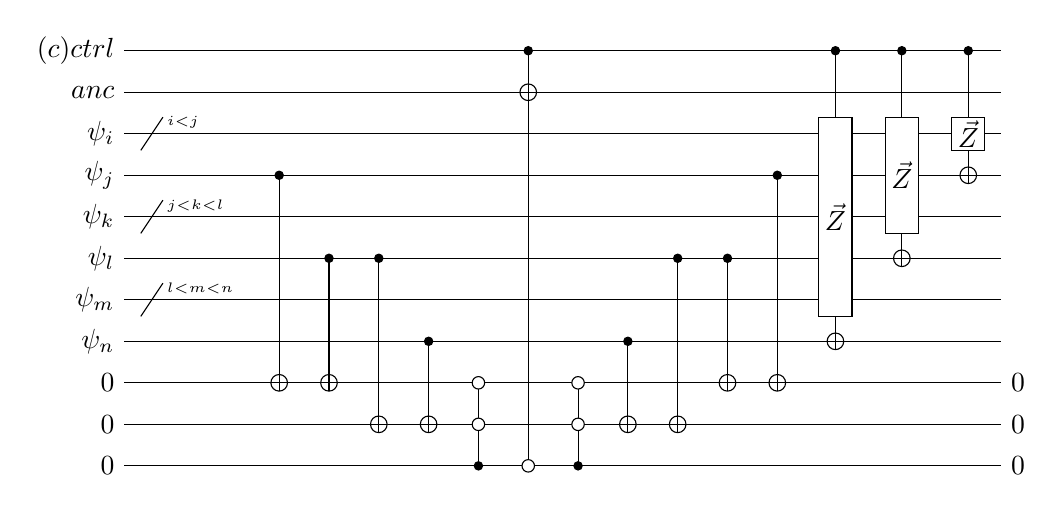
\begin{tikzpicture}[scale=1.000000,x=1pt,y=1pt]
\filldraw[color=white] (0.000000, -7.500000) rectangle (317.000000, 157.500000);
% Drawing wires
% Line 1: ctrl W \text{(c) }ctrl
\draw[color=black] (0.000000,150.000000) -- (317.000000,150.000000);
\draw[color=black] (0.000000,150.000000) node[left] {$\text{(c) }ctrl$};
% Line 2: anc W anc
\draw[color=black] (0.000000,135.000000) -- (317.000000,135.000000);
\draw[color=black] (0.000000,135.000000) node[left] {$anc$};
% Line 3: i W \psi_i
\draw[color=black] (0.000000,120.000000) -- (317.000000,120.000000);
\draw[color=black] (0.000000,120.000000) node[left] {$\psi_i$};
% Line 4: j W \psi_j
\draw[color=black] (0.000000,105.000000) -- (317.000000,105.000000);
\draw[color=black] (0.000000,105.000000) node[left] {$\psi_j$};
% Line 5: k W \psi_k
\draw[color=black] (0.000000,90.000000) -- (317.000000,90.000000);
\draw[color=black] (0.000000,90.000000) node[left] {$\psi_k$};
% Line 6: l W \psi_l
\draw[color=black] (0.000000,75.000000) -- (317.000000,75.000000);
\draw[color=black] (0.000000,75.000000) node[left] {$\psi_l$};
% Line 7: m W \psi_m
\draw[color=black] (0.000000,60.000000) -- (317.000000,60.000000);
\draw[color=black] (0.000000,60.000000) node[left] {$\psi_m$};
% Line 8: n W \psi_n
\draw[color=black] (0.000000,45.000000) -- (317.000000,45.000000);
\draw[color=black] (0.000000,45.000000) node[left] {$\psi_n$};
% Line 9: clean0 W 0 0
\draw[color=black] (0.000000,30.000000) -- (317.000000,30.000000);
\draw[color=black] (0.000000,30.000000) node[left] {$0$};
% Line 10: clean1 W 0 0
\draw[color=black] (0.000000,15.000000) -- (317.000000,15.000000);
\draw[color=black] (0.000000,15.000000) node[left] {$0$};
% Line 11: clean2 W 0 0
\draw[color=black] (0.000000,0.000000) -- (317.000000,0.000000);
\draw[color=black] (0.000000,0.000000) node[left] {$0$};
% Done with wires; drawing gates
% Line 13: i / ^{i<j}
\draw (6.000000, 114.000000) -- (14.000000, 126.000000);
\draw (12.000000, 123.000000) node[right] {$\scriptstyle{^{i<j}}$};
% Line 14: k / ^{j<k<l}
\draw (6.000000, 84.000000) -- (14.000000, 96.000000);
\draw (12.000000, 93.000000) node[right] {$\scriptstyle{^{j<k<l}}$};
% Line 15: m / ^{l<m<n}
\draw (6.000000, 54.000000) -- (14.000000, 66.000000);
\draw (12.000000, 63.000000) node[right] {$\scriptstyle{^{l<m<n}}$};
% Line 16: ctrl anc i j k l m n clean0 LABEL
% Line 17: j +clean0
\draw (56.000000,105.000000) -- (56.000000,30.000000);
\filldraw (56.000000, 105.000000) circle(1.500000pt);
\begin{scope}
\draw[fill=white] (56.000000, 30.000000) circle(3.000000pt);
\clip (56.000000, 30.000000) circle(3.000000pt);
\draw (53.000000, 30.000000) -- (59.000000, 30.000000);
\draw (56.000000, 27.000000) -- (56.000000, 33.000000);
\end{scope}
% Line 18: l +clean0
\draw (74.000000,75.000000) -- (74.000000,30.000000);
\filldraw (74.000000, 75.000000) circle(1.500000pt);
\begin{scope}
\draw[fill=white] (74.000000, 30.000000) circle(3.000000pt);
\clip (74.000000, 30.000000) circle(3.000000pt);
\draw (71.000000, 30.000000) -- (77.000000, 30.000000);
\draw (74.000000, 27.000000) -- (74.000000, 33.000000);
\end{scope}
% Line 19: l +clean1
\draw (92.000000,75.000000) -- (92.000000,15.000000);
\filldraw (92.000000, 75.000000) circle(1.500000pt);
\begin{scope}
\draw[fill=white] (92.000000, 15.000000) circle(3.000000pt);
\clip (92.000000, 15.000000) circle(3.000000pt);
\draw (89.000000, 15.000000) -- (95.000000, 15.000000);
\draw (92.000000, 12.000000) -- (92.000000, 18.000000);
\end{scope}
% Line 20: n +clean1
\draw (110.000000,45.000000) -- (110.000000,15.000000);
\filldraw (110.000000, 45.000000) circle(1.500000pt);
\begin{scope}
\draw[fill=white] (110.000000, 15.000000) circle(3.000000pt);
\clip (110.000000, 15.000000) circle(3.000000pt);
\draw (107.000000, 15.000000) -- (113.000000, 15.000000);
\draw (110.000000, 12.000000) -- (110.000000, 18.000000);
\end{scope}
% Line 21: -clean0 -clean1 clean2
\draw (128.000000,30.000000) -- (128.000000,0.000000);
\draw[fill=white] (128.000000, 30.000000) circle(2.250000pt);
\draw[fill=white] (128.000000, 15.000000) circle(2.250000pt);
\filldraw (128.000000, 0.000000) circle(1.500000pt);
% Line 22: ctrl -clean2 +anc
\draw (146.000000,150.000000) -- (146.000000,0.000000);
\filldraw (146.000000, 150.000000) circle(1.500000pt);
\draw[fill=white] (146.000000, 0.000000) circle(2.250000pt);
\begin{scope}
\draw[fill=white] (146.000000, 135.000000) circle(3.000000pt);
\clip (146.000000, 135.000000) circle(3.000000pt);
\draw (143.000000, 135.000000) -- (149.000000, 135.000000);
\draw (146.000000, 132.000000) -- (146.000000, 138.000000);
\end{scope}
% Line 23: -clean0 -clean1 clean2
\draw (164.000000,30.000000) -- (164.000000,0.000000);
\draw[fill=white] (164.000000, 30.000000) circle(2.250000pt);
\draw[fill=white] (164.000000, 15.000000) circle(2.250000pt);
\filldraw (164.000000, 0.000000) circle(1.500000pt);
% Line 24: n +clean1
\draw (182.000000,45.000000) -- (182.000000,15.000000);
\filldraw (182.000000, 45.000000) circle(1.500000pt);
\begin{scope}
\draw[fill=white] (182.000000, 15.000000) circle(3.000000pt);
\clip (182.000000, 15.000000) circle(3.000000pt);
\draw (179.000000, 15.000000) -- (185.000000, 15.000000);
\draw (182.000000, 12.000000) -- (182.000000, 18.000000);
\end{scope}
% Line 25: l +clean1
\draw (200.000000,75.000000) -- (200.000000,15.000000);
\filldraw (200.000000, 75.000000) circle(1.500000pt);
\begin{scope}
\draw[fill=white] (200.000000, 15.000000) circle(3.000000pt);
\clip (200.000000, 15.000000) circle(3.000000pt);
\draw (197.000000, 15.000000) -- (203.000000, 15.000000);
\draw (200.000000, 12.000000) -- (200.000000, 18.000000);
\end{scope}
% Line 26: l +clean0
\draw (218.000000,75.000000) -- (218.000000,30.000000);
\filldraw (218.000000, 75.000000) circle(1.500000pt);
\begin{scope}
\draw[fill=white] (218.000000, 30.000000) circle(3.000000pt);
\clip (218.000000, 30.000000) circle(3.000000pt);
\draw (215.000000, 30.000000) -- (221.000000, 30.000000);
\draw (218.000000, 27.000000) -- (218.000000, 33.000000);
\end{scope}
% Line 27: j +clean0
\draw (236.000000,105.000000) -- (236.000000,30.000000);
\filldraw (236.000000, 105.000000) circle(1.500000pt);
\begin{scope}
\draw[fill=white] (236.000000, 30.000000) circle(3.000000pt);
\clip (236.000000, 30.000000) circle(3.000000pt);
\draw (233.000000, 30.000000) -- (239.000000, 30.000000);
\draw (236.000000, 27.000000) -- (236.000000, 33.000000);
\end{scope}
% Line 29: i j k l m G $\vec{Z}$ ctrl +n
\draw (257.000000,150.000000) -- (257.000000,45.000000);
\begin{scope}
\draw[fill=white] (257.000000, 90.000000) +(-45.000000:8.485281pt and 50.911688pt) -- +(45.000000:8.485281pt and 50.911688pt) -- +(135.000000:8.485281pt and 50.911688pt) -- +(225.000000:8.485281pt and 50.911688pt) -- cycle;
\clip (257.000000, 90.000000) +(-45.000000:8.485281pt and 50.911688pt) -- +(45.000000:8.485281pt and 50.911688pt) -- +(135.000000:8.485281pt and 50.911688pt) -- +(225.000000:8.485281pt and 50.911688pt) -- cycle;
\draw (257.000000, 90.000000) node {$\vec{Z}$};
\end{scope}
\filldraw (257.000000, 150.000000) circle(1.500000pt);
\begin{scope}
\draw[fill=white] (257.000000, 45.000000) circle(3.000000pt);
\clip (257.000000, 45.000000) circle(3.000000pt);
\draw (254.000000, 45.000000) -- (260.000000, 45.000000);
\draw (257.000000, 42.000000) -- (257.000000, 48.000000);
\end{scope}
% Line 30: i j k G $\vec{Z}$ ctrl +l
\draw (281.000000,150.000000) -- (281.000000,75.000000);
\begin{scope}
\draw[fill=white] (281.000000, 105.000000) +(-45.000000:8.485281pt and 29.698485pt) -- +(45.000000:8.485281pt and 29.698485pt) -- +(135.000000:8.485281pt and 29.698485pt) -- +(225.000000:8.485281pt and 29.698485pt) -- cycle;
\clip (281.000000, 105.000000) +(-45.000000:8.485281pt and 29.698485pt) -- +(45.000000:8.485281pt and 29.698485pt) -- +(135.000000:8.485281pt and 29.698485pt) -- +(225.000000:8.485281pt and 29.698485pt) -- cycle;
\draw (281.000000, 105.000000) node {$\vec{Z}$};
\end{scope}
\filldraw (281.000000, 150.000000) circle(1.500000pt);
\begin{scope}
\draw[fill=white] (281.000000, 75.000000) circle(3.000000pt);
\clip (281.000000, 75.000000) circle(3.000000pt);
\draw (278.000000, 75.000000) -- (284.000000, 75.000000);
\draw (281.000000, 72.000000) -- (281.000000, 78.000000);
\end{scope}
% Line 31: i G $\vec{Z}$ ctrl +j
\draw (305.000000,150.000000) -- (305.000000,105.000000);
\begin{scope}
\draw[fill=white] (305.000000, 120.000000) +(-45.000000:8.485281pt and 8.485281pt) -- +(45.000000:8.485281pt and 8.485281pt) -- +(135.000000:8.485281pt and 8.485281pt) -- +(225.000000:8.485281pt and 8.485281pt) -- cycle;
\clip (305.000000, 120.000000) +(-45.000000:8.485281pt and 8.485281pt) -- +(45.000000:8.485281pt and 8.485281pt) -- +(135.000000:8.485281pt and 8.485281pt) -- +(225.000000:8.485281pt and 8.485281pt) -- cycle;
\draw (305.000000, 120.000000) node {$\vec{Z}$};
\end{scope}
\filldraw (305.000000, 150.000000) circle(1.500000pt);
\begin{scope}
\draw[fill=white] (305.000000, 105.000000) circle(3.000000pt);
\clip (305.000000, 105.000000) circle(3.000000pt);
\draw (302.000000, 105.000000) -- (308.000000, 105.000000);
\draw (305.000000, 102.000000) -- (305.000000, 108.000000);
\end{scope}
% Done with gates; drawing ending labels
\draw[color=black] (317.000000,30.000000) node[right] {$0$};
\draw[color=black] (317.000000,15.000000) node[right] {$0$};
\draw[color=black] (317.000000,0.000000) node[right] {$0$};
% Done with ending labels; drawing cut lines and comments
% Done with comments
\end{tikzpicture}

    \caption{
        \textbf{Block-Encoding Product of Fermionic Operators Plus Hermitian Conjugate}
        In (a), a block-encoding for the operator $b_j + b_j^\dagger$ is given.
        In (b), a block-encoding for the operator $b_j b_l + b_l^\dagger b_j^\dagger$ is given.
        In (c), a block-encoding for the operator $b_j b_l b_n + b_n^\dagger b_l^\dagger b_j^\dagger$ is given.
    }
    \label{fig:fermionic-be-lc-small}
\end{figure*}


Consider a linear combination of an individual fermionic ladder operator with its hermitian conjugate: $b_j^\dagger + b_j$.
The action of this operator on the two possible occupation states of the $j^\text{th}$ fermionic mode is given by:
\begin{equation}
    \label{eq:action-of-fermionic-op-plus-hc}
    \begin{split}
        (b_j^\dagger + b_j) \ket{\psi_{b_j}} = \begin{cases} 
            p(\psi) \ket{1} & \text{when $\ket{\psi_{b_j}}$ is $\ket{0}$} \\
            p(\psi) \ket{0} & \text{when $\ket{\psi_{b_j}}$ is $\ket{1}$} \\
                                        \end{cases}
    \end{split}
\end{equation}

An LCO construction using the block-encodings for these two ladder operators presented in the previous section would have a rescaling factor of $\lambda = 2$, require two block-encoding ancillae and two clean ancillae, and use $12$ T gates.
However, by considering the action of this operator (Eq. \ref{eq:action-of-fermionic-op-plus-hc}) on the active mode, a more efficient block-encoding can be constructed.
A Pauli $X$ gate can be applied to the $j^\text{th}$ mode to flip the occupation and a string of Pauli $Z$ gates can be applied on each fermionic mode with index $i < j$ to apply the potential phase flip induced by $p(\psi)$.
This results in the same decomposition one would arrive at using the Jordan-Wigner transformation ($\vec{Z}X_j$).
A circuit diagram for this block-encoding is shown in subfigure \ref{fig:fermionic-be-lc-small}a.
This block-encoding circuit has an optimal rescaling factor ($\lambda = 1$), requires zero block-encoding ancillae and zero clean ancillae, and uses zero non-Clifford operations.

For a two-body fermionic operator and its hermitian conjugate ($b_j b_l + b_l^\dagger b_j^\dagger$) with $j \neq l$ we arrive at a construction that differs from the Jordan-Wigner transformation.
We begin by swapping the operators in the second term using the anticommutation relations to ensure that the order in which the corresponding operators appear in each term is the same: $b_j b_l - b_j^\dagger b_l^\dagger$.
In the circuit, the order in which the system is updated based on the ladder operators is fixed so it must be consistent for both terms.
This reordering means that the potential phase flips caused by each ladder operator will be consistent for both terms since the order at which the operators are applied onto the system is consistent.
The action of the joined operator on the possible occupation states of the $j^\text{th}$ and $l^\text{th}$ fermionic modes is given by:
\begin{equation}
    \begin{split}
        (b_j b_l - b_j^\dagger b_l^\dagger) \ket{\psi_{b_l} \psi_{b_j}} = \\
        \begin{cases} 
            - p(\psi) \ket{11} & \text{when $\ket{\psi_{b_l} \psi_{b_j}}$ is $\ket{00}$} \\
            \hspace{0.75em} p(\psi) \ket{00} & \text{when $\ket{\psi_{b_l} \psi_{b_j}}$ is $\ket{11}$} \\
            \hspace{2em} 0 & \text{when $\ket{\psi_{b_l} \psi_{b_j}}$ is $\ket{01}$} \\
            \hspace{2em} 0 & \text{when $\ket{\psi_{b_l} \psi_{b_j}}$ is $\ket{10}$} \\
        \end{cases}
    \end{split}
\end{equation}
From this perspective, it is clear that the action of this operator on the system is determined by the parity of the two active fermionic modes.

In subfigure \ref{fig:fermionic-be-lc-small}b, we give a circuit diagram for block-encoding this two-body operator.
The parity of the active modes can be computed using a CNOT gate controlled on the $j^\text{th}$ mode, targeting the $l^\text{th}$ mode.
If the control qubit is on and $\ket{\psi_{b_l}}$ is in the $\ket{1}$ state (odd parity), then the block-encoding ancilla is flipped to push that branch of the wavefunction outside of the encoded subspace.
After this operation, the parity can be uncomputed, returning the qubit storing the occupation of the $l^\text{th}$ mode to its original state.
Next, a $CZ$ gate that is $0$-controlled on the $j^\text{th}$ fermionic mode and $1$-controlled on the control qubit applies the desired sign flip corresponding to the term $- b_j^\dagger b_l^\dagger$.
Lastly, a series of $\vec{Z}X$ operators are applied to each active mode in the order at which the operators would be applied onto the system (right to left).

\begin{figure}
    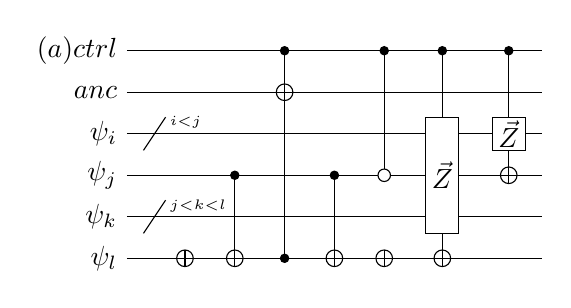
\begin{tikzpicture}[scale=1.000000,x=1pt,y=1pt]
\filldraw[color=white] (0.000000, -7.500000) rectangle (150.000000, 82.500000);
% Drawing wires
% Line 1: c W \text{(a) }ctrl
\draw[color=black] (0.000000,75.000000) -- (150.000000,75.000000);
\draw[color=black] (0.000000,75.000000) node[left] {$\text{(a) }ctrl$};
% Line 2: a W anc
\draw[color=black] (0.000000,60.000000) -- (150.000000,60.000000);
\draw[color=black] (0.000000,60.000000) node[left] {$anc$};
% Line 3: i W \psi_i
\draw[color=black] (0.000000,45.000000) -- (150.000000,45.000000);
\draw[color=black] (0.000000,45.000000) node[left] {$\psi_i$};
% Line 4: j W \psi_j
\draw[color=black] (0.000000,30.000000) -- (150.000000,30.000000);
\draw[color=black] (0.000000,30.000000) node[left] {$\psi_j$};
% Line 5: k W \psi_k
\draw[color=black] (0.000000,15.000000) -- (150.000000,15.000000);
\draw[color=black] (0.000000,15.000000) node[left] {$\psi_k$};
% Line 6: l W \psi_l
\draw[color=black] (0.000000,0.000000) -- (150.000000,0.000000);
\draw[color=black] (0.000000,0.000000) node[left] {$\psi_l$};
% Done with wires; drawing gates
% Line 8: i / ^{i<j}
\draw (6.000000, 39.000000) -- (14.000000, 51.000000);
\draw (12.000000, 48.000000) node[right] {$\scriptstyle{^{i<j}}$};
% Line 9: k / ^{j<k<l}
\draw (6.000000, 9.000000) -- (14.000000, 21.000000);
\draw (12.000000, 18.000000) node[right] {$\scriptstyle{^{j<k<l}}$};
% Line 10: c a i j k l LABEL width=-20
% Line 12: +l
\begin{scope}
\draw[fill=white] (21.000000, 0.000000) circle(3.000000pt);
\clip (21.000000, 0.000000) circle(3.000000pt);
\draw (18.000000, 0.000000) -- (24.000000, 0.000000);
\draw (21.000000, -3.000000) -- (21.000000, 3.000000);
\end{scope}
% Line 13: j +l
\draw (39.000000,30.000000) -- (39.000000,0.000000);
\filldraw (39.000000, 30.000000) circle(1.500000pt);
\begin{scope}
\draw[fill=white] (39.000000, 0.000000) circle(3.000000pt);
\clip (39.000000, 0.000000) circle(3.000000pt);
\draw (36.000000, 0.000000) -- (42.000000, 0.000000);
\draw (39.000000, -3.000000) -- (39.000000, 3.000000);
\end{scope}
% Line 14: c l +a
\draw (57.000000,75.000000) -- (57.000000,0.000000);
\filldraw (57.000000, 75.000000) circle(1.500000pt);
\filldraw (57.000000, 0.000000) circle(1.500000pt);
\begin{scope}
\draw[fill=white] (57.000000, 60.000000) circle(3.000000pt);
\clip (57.000000, 60.000000) circle(3.000000pt);
\draw (54.000000, 60.000000) -- (60.000000, 60.000000);
\draw (57.000000, 57.000000) -- (57.000000, 63.000000);
\end{scope}
% Line 15: j +l
\draw (75.000000,30.000000) -- (75.000000,0.000000);
\filldraw (75.000000, 30.000000) circle(1.500000pt);
\begin{scope}
\draw[fill=white] (75.000000, 0.000000) circle(3.000000pt);
\clip (75.000000, 0.000000) circle(3.000000pt);
\draw (72.000000, 0.000000) -- (78.000000, 0.000000);
\draw (75.000000, -3.000000) -- (75.000000, 3.000000);
\end{scope}
% Line 16: +l
\begin{scope}
\draw[fill=white] (93.000000, 0.000000) circle(3.000000pt);
\clip (93.000000, 0.000000) circle(3.000000pt);
\draw (90.000000, 0.000000) -- (96.000000, 0.000000);
\draw (93.000000, -3.000000) -- (93.000000, 3.000000);
\end{scope}
% Line 18: c -j
\draw (93.000000,75.000000) -- (93.000000,30.000000);
\filldraw (93.000000, 75.000000) circle(1.500000pt);
\draw[fill=white] (93.000000, 30.000000) circle(2.250000pt);
% Line 20: i j k G $\vec{Z}$ c +l
\draw (114.000000,75.000000) -- (114.000000,0.000000);
\begin{scope}
\draw[fill=white] (114.000000, 30.000000) +(-45.000000:8.485281pt and 29.698485pt) -- +(45.000000:8.485281pt and 29.698485pt) -- +(135.000000:8.485281pt and 29.698485pt) -- +(225.000000:8.485281pt and 29.698485pt) -- cycle;
\clip (114.000000, 30.000000) +(-45.000000:8.485281pt and 29.698485pt) -- +(45.000000:8.485281pt and 29.698485pt) -- +(135.000000:8.485281pt and 29.698485pt) -- +(225.000000:8.485281pt and 29.698485pt) -- cycle;
\draw (114.000000, 30.000000) node {$\vec{Z}$};
\end{scope}
\filldraw (114.000000, 75.000000) circle(1.500000pt);
\begin{scope}
\draw[fill=white] (114.000000, 0.000000) circle(3.000000pt);
\clip (114.000000, 0.000000) circle(3.000000pt);
\draw (111.000000, 0.000000) -- (117.000000, 0.000000);
\draw (114.000000, -3.000000) -- (114.000000, 3.000000);
\end{scope}
% Line 21: i G $\vec{Z}$ c +j
\draw (138.000000,75.000000) -- (138.000000,30.000000);
\begin{scope}
\draw[fill=white] (138.000000, 45.000000) +(-45.000000:8.485281pt and 8.485281pt) -- +(45.000000:8.485281pt and 8.485281pt) -- +(135.000000:8.485281pt and 8.485281pt) -- +(225.000000:8.485281pt and 8.485281pt) -- cycle;
\clip (138.000000, 45.000000) +(-45.000000:8.485281pt and 8.485281pt) -- +(45.000000:8.485281pt and 8.485281pt) -- +(135.000000:8.485281pt and 8.485281pt) -- +(225.000000:8.485281pt and 8.485281pt) -- cycle;
\draw (138.000000, 45.000000) node {$\vec{Z}$};
\end{scope}
\filldraw (138.000000, 75.000000) circle(1.500000pt);
\begin{scope}
\draw[fill=white] (138.000000, 30.000000) circle(3.000000pt);
\clip (138.000000, 30.000000) circle(3.000000pt);
\draw (135.000000, 30.000000) -- (141.000000, 30.000000);
\draw (138.000000, 27.000000) -- (138.000000, 33.000000);
\end{scope}
% Done with gates; drawing ending labels
% Done with ending labels; drawing cut lines and comments
% Done with comments
\end{tikzpicture}

    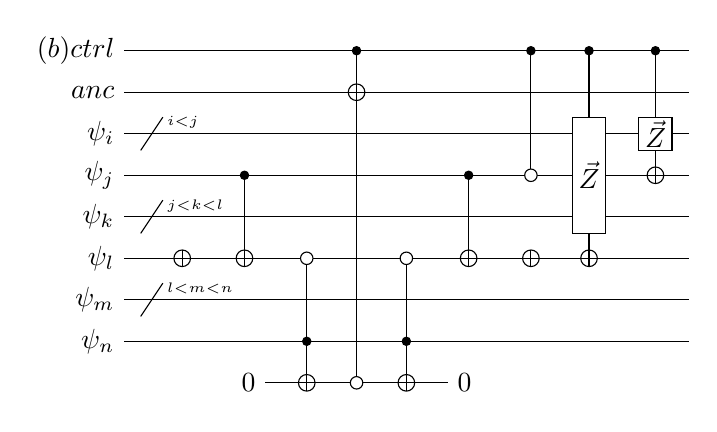
\begin{tikzpicture}[scale=1.000000,x=1pt,y=1pt]
\filldraw[color=white] (0.000000, -7.500000) rectangle (204.000000, 127.500000);
% Drawing wires
% Line 1: c W \text{(b) }ctrl
\draw[color=black] (0.000000,120.000000) -- (204.000000,120.000000);
\draw[color=black] (0.000000,120.000000) node[left] {$\text{(b) }ctrl$};
% Line 2: a W anc
\draw[color=black] (0.000000,105.000000) -- (204.000000,105.000000);
\draw[color=black] (0.000000,105.000000) node[left] {$anc$};
% Line 3: i W \psi_i
\draw[color=black] (0.000000,90.000000) -- (204.000000,90.000000);
\draw[color=black] (0.000000,90.000000) node[left] {$\psi_i$};
% Line 4: j W \psi_j
\draw[color=black] (0.000000,75.000000) -- (204.000000,75.000000);
\draw[color=black] (0.000000,75.000000) node[left] {$\psi_j$};
% Line 5: k W \psi_k
\draw[color=black] (0.000000,60.000000) -- (204.000000,60.000000);
\draw[color=black] (0.000000,60.000000) node[left] {$\psi_k$};
% Line 6: l W \psi_l
\draw[color=black] (0.000000,45.000000) -- (204.000000,45.000000);
\draw[color=black] (0.000000,45.000000) node[left] {$\psi_l$};
% Line 7: m W \psi_m
\draw[color=black] (0.000000,30.000000) -- (204.000000,30.000000);
\draw[color=black] (0.000000,30.000000) node[left] {$\psi_m$};
% Line 8: n W \psi_n
\draw[color=black] (0.000000,15.000000) -- (204.000000,15.000000);
\draw[color=black] (0.000000,15.000000) node[left] {$\psi_n$};
% Line 9: clean W 0 0
\draw[color=black] (43.500000,0.000000) -- (124.500000,0.000000);
% Done with wires; drawing gates
% Line 11: i / ^{i<j}
\draw (6.000000, 84.000000) -- (14.000000, 96.000000);
\draw (12.000000, 93.000000) node[right] {$\scriptstyle{^{i<j}}$};
% Line 12: k / ^{j<k<l}
\draw (6.000000, 54.000000) -- (14.000000, 66.000000);
\draw (12.000000, 63.000000) node[right] {$\scriptstyle{^{j<k<l}}$};
% Line 13: m / ^{l<m<n}
\draw (6.000000, 24.000000) -- (14.000000, 36.000000);
\draw (12.000000, 33.000000) node[right] {$\scriptstyle{^{l<m<n}}$};
% Line 14: c a i j k l m n clean LABEL width=-20
% Line 16: +l
\begin{scope}
\draw[fill=white] (21.000000, 45.000000) circle(3.000000pt);
\clip (21.000000, 45.000000) circle(3.000000pt);
\draw (18.000000, 45.000000) -- (24.000000, 45.000000);
\draw (21.000000, 42.000000) -- (21.000000, 48.000000);
\end{scope}
% Line 17: j +l
\draw (43.500000,75.000000) -- (43.500000,45.000000);
\filldraw (43.500000, 75.000000) circle(1.500000pt);
\begin{scope}
\draw[fill=white] (43.500000, 45.000000) circle(3.000000pt);
\clip (43.500000, 45.000000) circle(3.000000pt);
\draw (40.500000, 45.000000) -- (46.500000, 45.000000);
\draw (43.500000, 42.000000) -- (43.500000, 48.000000);
\end{scope}
% Line 18: clean START
\draw[color=black] (51.000000,0.000000) node[fill=white,left,minimum height=15.000000pt,minimum width=15.000000pt,inner sep=0pt] {\phantom{$0$}};
\draw[color=black] (51.000000,0.000000) node[left] {$0$};
% Line 19: n -l +clean
\draw (66.000000,45.000000) -- (66.000000,0.000000);
\filldraw (66.000000, 15.000000) circle(1.500000pt);
\draw[fill=white] (66.000000, 45.000000) circle(2.250000pt);
\begin{scope}
\draw[fill=white] (66.000000, 0.000000) circle(3.000000pt);
\clip (66.000000, 0.000000) circle(3.000000pt);
\draw (63.000000, 0.000000) -- (69.000000, 0.000000);
\draw (66.000000, -3.000000) -- (66.000000, 3.000000);
\end{scope}
% Line 20: c -clean +a
\draw (84.000000,120.000000) -- (84.000000,0.000000);
\filldraw (84.000000, 120.000000) circle(1.500000pt);
\draw[fill=white] (84.000000, 0.000000) circle(2.250000pt);
\begin{scope}
\draw[fill=white] (84.000000, 105.000000) circle(3.000000pt);
\clip (84.000000, 105.000000) circle(3.000000pt);
\draw (81.000000, 105.000000) -- (87.000000, 105.000000);
\draw (84.000000, 102.000000) -- (84.000000, 108.000000);
\end{scope}
% Line 21: n -l +clean
\draw (102.000000,45.000000) -- (102.000000,0.000000);
\filldraw (102.000000, 15.000000) circle(1.500000pt);
\draw[fill=white] (102.000000, 45.000000) circle(2.250000pt);
\begin{scope}
\draw[fill=white] (102.000000, 0.000000) circle(3.000000pt);
\clip (102.000000, 0.000000) circle(3.000000pt);
\draw (99.000000, 0.000000) -- (105.000000, 0.000000);
\draw (102.000000, -3.000000) -- (102.000000, 3.000000);
\end{scope}
% Line 22: clean END
\draw[color=black] (117.000000,0.000000) node[fill=white,right,minimum height=15.000000pt,minimum width=15.000000pt,inner sep=0pt] {\phantom{$0$}};
\draw[color=black] (117.000000,0.000000) node[right] {$0$};
% Line 23: j +l
\draw (124.500000,75.000000) -- (124.500000,45.000000);
\filldraw (124.500000, 75.000000) circle(1.500000pt);
\begin{scope}
\draw[fill=white] (124.500000, 45.000000) circle(3.000000pt);
\clip (124.500000, 45.000000) circle(3.000000pt);
\draw (121.500000, 45.000000) -- (127.500000, 45.000000);
\draw (124.500000, 42.000000) -- (124.500000, 48.000000);
\end{scope}
% Line 24: +l
\begin{scope}
\draw[fill=white] (147.000000, 45.000000) circle(3.000000pt);
\clip (147.000000, 45.000000) circle(3.000000pt);
\draw (144.000000, 45.000000) -- (150.000000, 45.000000);
\draw (147.000000, 42.000000) -- (147.000000, 48.000000);
\end{scope}
% Line 26: c -j
\draw (147.000000,120.000000) -- (147.000000,75.000000);
\filldraw (147.000000, 120.000000) circle(1.500000pt);
\draw[fill=white] (147.000000, 75.000000) circle(2.250000pt);
% Line 28: i j k G $\vec{Z}$ c +l
\draw (168.000000,120.000000) -- (168.000000,45.000000);
\begin{scope}
\draw[fill=white] (168.000000, 75.000000) +(-45.000000:8.485281pt and 29.698485pt) -- +(45.000000:8.485281pt and 29.698485pt) -- +(135.000000:8.485281pt and 29.698485pt) -- +(225.000000:8.485281pt and 29.698485pt) -- cycle;
\clip (168.000000, 75.000000) +(-45.000000:8.485281pt and 29.698485pt) -- +(45.000000:8.485281pt and 29.698485pt) -- +(135.000000:8.485281pt and 29.698485pt) -- +(225.000000:8.485281pt and 29.698485pt) -- cycle;
\draw (168.000000, 75.000000) node {$\vec{Z}$};
\end{scope}
\filldraw (168.000000, 120.000000) circle(1.500000pt);
\begin{scope}
\draw[fill=white] (168.000000, 45.000000) circle(3.000000pt);
\clip (168.000000, 45.000000) circle(3.000000pt);
\draw (165.000000, 45.000000) -- (171.000000, 45.000000);
\draw (168.000000, 42.000000) -- (168.000000, 48.000000);
\end{scope}
% Line 29: i G $\vec{Z}$ c +j
\draw (192.000000,120.000000) -- (192.000000,75.000000);
\begin{scope}
\draw[fill=white] (192.000000, 90.000000) +(-45.000000:8.485281pt and 8.485281pt) -- +(45.000000:8.485281pt and 8.485281pt) -- +(135.000000:8.485281pt and 8.485281pt) -- +(225.000000:8.485281pt and 8.485281pt) -- cycle;
\clip (192.000000, 90.000000) +(-45.000000:8.485281pt and 8.485281pt) -- +(45.000000:8.485281pt and 8.485281pt) -- +(135.000000:8.485281pt and 8.485281pt) -- +(225.000000:8.485281pt and 8.485281pt) -- cycle;
\draw (192.000000, 90.000000) node {$\vec{Z}$};
\end{scope}
\filldraw (192.000000, 120.000000) circle(1.500000pt);
\begin{scope}
\draw[fill=white] (192.000000, 75.000000) circle(3.000000pt);
\clip (192.000000, 75.000000) circle(3.000000pt);
\draw (189.000000, 75.000000) -- (195.000000, 75.000000);
\draw (192.000000, 72.000000) -- (192.000000, 78.000000);
\end{scope}
% Done with gates; drawing ending labels
% Done with ending labels; drawing cut lines and comments
% Done with comments
\end{tikzpicture}

    \caption{
        \textbf{Block-Encoding Product of Fermionic Operators Plus Hermitian Conjugate (modifications)}
        In (a), a block-encoding for the operator $b_j b_l^\dagger + b_l b_j^\dagger$ is given.
        In (b), a block-encoding for the operator $b_j b_l^\dagger b_n^\dagger b_n + b_n^\dagger b_n b_l b_j^\dagger$ is given.
    }
    \label{fig:fermionic-be-lc-modifications}
\end{figure}

For an operator of the form $b_j b_l^\dagger + b_l b_j^\dagger$, we can construct a similar block-encoding with a slight modification.
In this case, we simply flip the occupation of the $l^\text{th}$ mode using a Pauli $X$ gate before we compute the parity of the modes.
The circuit diagram for block-encoding this operator is given in subfigure \ref{fig:fermionic-be-lc-modifications}a.

Likewise, if a number operator is included in a term, this can be accounted for by including a $1$-control on that mode when determining if the block-encoding ancilla should be flipped and excluding that mode from any parity computations.
An example circuit diagram for an operator including a number operator is given in subfigure \ref{fig:fermionic-be-lc-modifications}b.

\begin{figure*}
    \definecolor{tblue}{RGB}{61,142,221}
\definecolor{torange}{RGB}{253,143,41}
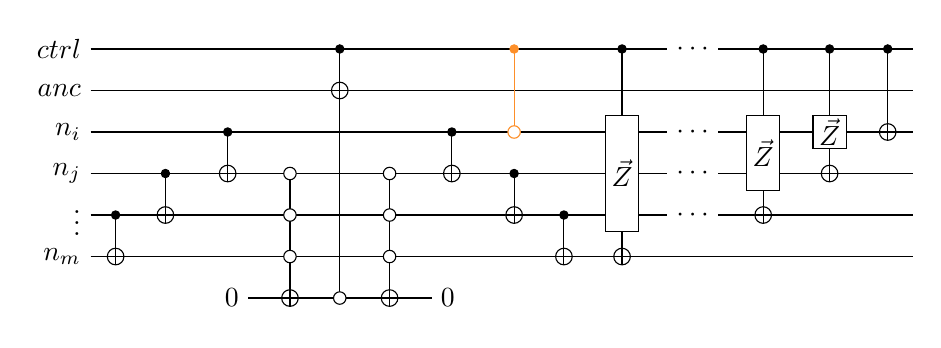
\begin{tikzpicture}[scale=1.000000,x=1pt,y=1pt]
\filldraw[color=white] (0.000000, -7.500000) rectangle (297.000000, 97.500000);
% Drawing wires
% Line 4: ctrl W ctrl
\draw[color=black] (0.000000,90.000000) -- (297.000000,90.000000);
\draw[color=black] (0.000000,90.000000) node[left] {$ctrl$};
% Line 5: anc W anc
\draw[color=black] (0.000000,75.000000) -- (297.000000,75.000000);
\draw[color=black] (0.000000,75.000000) node[left] {$anc$};
% Line 6: i W n_i
\draw[color=black] (0.000000,60.000000) -- (297.000000,60.000000);
\draw[color=black] (0.000000,60.000000) node[left] {$n_i$};
% Line 7: j W n_j
\draw[color=black] (0.000000,45.000000) -- (297.000000,45.000000);
\draw[color=black] (0.000000,45.000000) node[left] {$n_j$};
% Line 8: sys W \vdots
\draw[color=black] (0.000000,30.000000) -- (297.000000,30.000000);
\draw[color=black] (0.000000,30.000000) node[left] {$\vdots$};
% Line 9: m W n_m
\draw[color=black] (0.000000,15.000000) -- (297.000000,15.000000);
\draw[color=black] (0.000000,15.000000) node[left] {$n_m$};
% Line 10: clean W 0 0
\draw[color=black] (49.500000,0.000000) -- (130.500000,0.000000);
% Done with wires; drawing gates
% Line 12: sys +m
\draw (9.000000,30.000000) -- (9.000000,15.000000);
\filldraw (9.000000, 30.000000) circle(1.500000pt);
\begin{scope}
\draw[fill=white] (9.000000, 15.000000) circle(3.000000pt);
\clip (9.000000, 15.000000) circle(3.000000pt);
\draw (6.000000, 15.000000) -- (12.000000, 15.000000);
\draw (9.000000, 12.000000) -- (9.000000, 18.000000);
\end{scope}
% Line 13: j +sys
\draw (27.000000,45.000000) -- (27.000000,30.000000);
\filldraw (27.000000, 45.000000) circle(1.500000pt);
\begin{scope}
\draw[fill=white] (27.000000, 30.000000) circle(3.000000pt);
\clip (27.000000, 30.000000) circle(3.000000pt);
\draw (24.000000, 30.000000) -- (30.000000, 30.000000);
\draw (27.000000, 27.000000) -- (27.000000, 33.000000);
\end{scope}
% Line 14: i +j
\draw (49.500000,60.000000) -- (49.500000,45.000000);
\filldraw (49.500000, 60.000000) circle(1.500000pt);
\begin{scope}
\draw[fill=white] (49.500000, 45.000000) circle(3.000000pt);
\clip (49.500000, 45.000000) circle(3.000000pt);
\draw (46.500000, 45.000000) -- (52.500000, 45.000000);
\draw (49.500000, 42.000000) -- (49.500000, 48.000000);
\end{scope}
% Line 16: clean START
\draw[color=black] (57.000000,0.000000) node[fill=white,left,minimum height=15.000000pt,minimum width=15.000000pt,inner sep=0pt] {\phantom{$0$}};
\draw[color=black] (57.000000,0.000000) node[left] {$0$};
% Line 17: -j -sys -m +clean
\draw (72.000000,45.000000) -- (72.000000,0.000000);
\draw[fill=white] (72.000000, 45.000000) circle(2.250000pt);
\draw[fill=white] (72.000000, 30.000000) circle(2.250000pt);
\draw[fill=white] (72.000000, 15.000000) circle(2.250000pt);
\begin{scope}
\draw[fill=white] (72.000000, 0.000000) circle(3.000000pt);
\clip (72.000000, 0.000000) circle(3.000000pt);
\draw (69.000000, 0.000000) -- (75.000000, 0.000000);
\draw (72.000000, -3.000000) -- (72.000000, 3.000000);
\end{scope}
% Line 18: ctrl -clean +anc
\draw (90.000000,90.000000) -- (90.000000,0.000000);
\filldraw (90.000000, 90.000000) circle(1.500000pt);
\draw[fill=white] (90.000000, 0.000000) circle(2.250000pt);
\begin{scope}
\draw[fill=white] (90.000000, 75.000000) circle(3.000000pt);
\clip (90.000000, 75.000000) circle(3.000000pt);
\draw (87.000000, 75.000000) -- (93.000000, 75.000000);
\draw (90.000000, 72.000000) -- (90.000000, 78.000000);
\end{scope}
% Line 19: -j -sys -m +clean
\draw (108.000000,45.000000) -- (108.000000,0.000000);
\draw[fill=white] (108.000000, 45.000000) circle(2.250000pt);
\draw[fill=white] (108.000000, 30.000000) circle(2.250000pt);
\draw[fill=white] (108.000000, 15.000000) circle(2.250000pt);
\begin{scope}
\draw[fill=white] (108.000000, 0.000000) circle(3.000000pt);
\clip (108.000000, 0.000000) circle(3.000000pt);
\draw (105.000000, 0.000000) -- (111.000000, 0.000000);
\draw (108.000000, -3.000000) -- (108.000000, 3.000000);
\end{scope}
% Line 20: clean END
\draw[color=black] (123.000000,0.000000) node[fill=white,right,minimum height=15.000000pt,minimum width=15.000000pt,inner sep=0pt] {\phantom{$0$}};
\draw[color=black] (123.000000,0.000000) node[right] {$0$};
% Line 22: i +j
\draw (130.500000,60.000000) -- (130.500000,45.000000);
\filldraw (130.500000, 60.000000) circle(1.500000pt);
\begin{scope}
\draw[fill=white] (130.500000, 45.000000) circle(3.000000pt);
\clip (130.500000, 45.000000) circle(3.000000pt);
\draw (127.500000, 45.000000) -- (133.500000, 45.000000);
\draw (130.500000, 42.000000) -- (130.500000, 48.000000);
\end{scope}
% Line 23: j +sys
\draw (153.000000,45.000000) -- (153.000000,30.000000);
\filldraw (153.000000, 45.000000) circle(1.500000pt);
\begin{scope}
\draw[fill=white] (153.000000, 30.000000) circle(3.000000pt);
\clip (153.000000, 30.000000) circle(3.000000pt);
\draw (150.000000, 30.000000) -- (156.000000, 30.000000);
\draw (153.000000, 27.000000) -- (153.000000, 33.000000);
\end{scope}
% Line 27: ctrl -i color=torange
\begin{scope}[color=torange]
\draw (153.000000,90.000000) -- (153.000000,60.000000);
\filldraw (153.000000, 90.000000) circle(1.500000pt);
\draw[fill=white] (153.000000, 60.000000) circle(2.250000pt);
\end{scope}
% Line 24: sys +m
\draw (171.000000,30.000000) -- (171.000000,15.000000);
\filldraw (171.000000, 30.000000) circle(1.500000pt);
\begin{scope}
\draw[fill=white] (171.000000, 15.000000) circle(3.000000pt);
\clip (171.000000, 15.000000) circle(3.000000pt);
\draw (168.000000, 15.000000) -- (174.000000, 15.000000);
\draw (171.000000, 12.000000) -- (171.000000, 18.000000);
\end{scope}
% Line 29: i j sys G $\vec{Z}$ ctrl +m
\draw (192.000000,90.000000) -- (192.000000,15.000000);
\begin{scope}
\draw[fill=white] (192.000000, 45.000000) +(-45.000000:8.485281pt and 29.698485pt) -- +(45.000000:8.485281pt and 29.698485pt) -- +(135.000000:8.485281pt and 29.698485pt) -- +(225.000000:8.485281pt and 29.698485pt) -- cycle;
\clip (192.000000, 45.000000) +(-45.000000:8.485281pt and 29.698485pt) -- +(45.000000:8.485281pt and 29.698485pt) -- +(135.000000:8.485281pt and 29.698485pt) -- +(225.000000:8.485281pt and 29.698485pt) -- cycle;
\draw (192.000000, 45.000000) node {$\vec{Z}$};
\end{scope}
\filldraw (192.000000, 90.000000) circle(1.500000pt);
\begin{scope}
\draw[fill=white] (192.000000, 15.000000) circle(3.000000pt);
\clip (192.000000, 15.000000) circle(3.000000pt);
\draw (189.000000, 15.000000) -- (195.000000, 15.000000);
\draw (192.000000, 12.000000) -- (192.000000, 18.000000);
\end{scope}
% Line 30: ctrl i j sys LABEL ...
\draw[color=black] (217.500000, 90.000000) node [fill=white] {$\cdots$};
\draw[color=black] (217.500000, 60.000000) node [fill=white] {$\cdots$};
\draw[color=black] (217.500000, 45.000000) node [fill=white] {$\cdots$};
\draw[color=black] (217.500000, 30.000000) node [fill=white] {$\cdots$};
% Line 31: i j G $\vec{Z}$ ctrl +sys
\draw (243.000000,90.000000) -- (243.000000,30.000000);
\begin{scope}
\draw[fill=white] (243.000000, 52.500000) +(-45.000000:8.485281pt and 19.091883pt) -- +(45.000000:8.485281pt and 19.091883pt) -- +(135.000000:8.485281pt and 19.091883pt) -- +(225.000000:8.485281pt and 19.091883pt) -- cycle;
\clip (243.000000, 52.500000) +(-45.000000:8.485281pt and 19.091883pt) -- +(45.000000:8.485281pt and 19.091883pt) -- +(135.000000:8.485281pt and 19.091883pt) -- +(225.000000:8.485281pt and 19.091883pt) -- cycle;
\draw (243.000000, 52.500000) node {$\vec{Z}$};
\end{scope}
\filldraw (243.000000, 90.000000) circle(1.500000pt);
\begin{scope}
\draw[fill=white] (243.000000, 30.000000) circle(3.000000pt);
\clip (243.000000, 30.000000) circle(3.000000pt);
\draw (240.000000, 30.000000) -- (246.000000, 30.000000);
\draw (243.000000, 27.000000) -- (243.000000, 33.000000);
\end{scope}
% Line 32: i G $\vec{Z}$ ctrl +j
\draw (267.000000,90.000000) -- (267.000000,45.000000);
\begin{scope}
\draw[fill=white] (267.000000, 60.000000) +(-45.000000:8.485281pt and 8.485281pt) -- +(45.000000:8.485281pt and 8.485281pt) -- +(135.000000:8.485281pt and 8.485281pt) -- +(225.000000:8.485281pt and 8.485281pt) -- cycle;
\clip (267.000000, 60.000000) +(-45.000000:8.485281pt and 8.485281pt) -- +(45.000000:8.485281pt and 8.485281pt) -- +(135.000000:8.485281pt and 8.485281pt) -- +(225.000000:8.485281pt and 8.485281pt) -- cycle;
\draw (267.000000, 60.000000) node {$\vec{Z}$};
\end{scope}
\filldraw (267.000000, 90.000000) circle(1.500000pt);
\begin{scope}
\draw[fill=white] (267.000000, 45.000000) circle(3.000000pt);
\clip (267.000000, 45.000000) circle(3.000000pt);
\draw (264.000000, 45.000000) -- (270.000000, 45.000000);
\draw (267.000000, 42.000000) -- (267.000000, 48.000000);
\end{scope}
% Line 33: ctrl +i
\draw (288.000000,90.000000) -- (288.000000,60.000000);
\filldraw (288.000000, 90.000000) circle(1.500000pt);
\begin{scope}
\draw[fill=white] (288.000000, 60.000000) circle(3.000000pt);
\clip (288.000000, 60.000000) circle(3.000000pt);
\draw (285.000000, 60.000000) -- (291.000000, 60.000000);
\draw (288.000000, 57.000000) -- (288.000000, 63.000000);
\end{scope}
% Done with gates; drawing ending labels
% Done with ending labels; drawing cut lines and comments
% Done with comments
\end{tikzpicture}

    \caption{
        \textbf{Generalized Block-Encoding for Product of Fermionic Operators Plus Hermitian Conjugate}
        A block-encoding for the operator $b_i b_j ... b_m + b_m^\dagger ... b_j^\dagger b_i^\dagger$ is given.
        The $CZ$ gate highlighted in orange is present only if the swapping on the order of the operators in the second term induces a negative sign on the second term (an odd number of swaps are required to reorder the ladder operators).
        Block-encodings for similar operators such as those that include number operators or different arrangements of the creation and annihilation operators can be accounted for using the modifications shown in Figure \ref{fig:fermionic-be-lc-modifications}.
    }
    \label{fig:fermionic-be-lc}
\end{figure*}

The construction of these block-encoding circuits can be generalized to any operator that is a product of fermionic operators plus its hermitian conjugate.
An example circuit diagram for this generalized construction is shown in Figure \ref{fig:fermionic-be-lc}.
If $C$ represents the number of active modes excluding modes where a number operator is acting on the mode, then the $CZ$ gate is present only if $(C \text{ choose } 2)$ is odd.
These block-encoding circuits will all have optimal rescaling factors ($\lambda=1$), require one block-encoding ancilla and $B - 1$ clean ancillae, and use $4(B-1)$ T gates.

\begin{figure}
    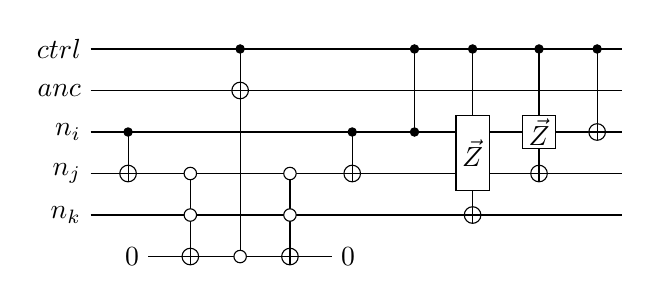
\begin{tikzpicture}[scale=1.000000,x=1pt,y=1pt]
\filldraw[color=white] (0.000000, -7.500000) rectangle (192.000000, 82.500000);
% Drawing wires
% Line 1: ctrl W ctrl
\draw[color=black] (0.000000,75.000000) -- (192.000000,75.000000);
\draw[color=black] (0.000000,75.000000) node[left] {$ctrl$};
% Line 2: anc W anc
\draw[color=black] (0.000000,60.000000) -- (192.000000,60.000000);
\draw[color=black] (0.000000,60.000000) node[left] {$anc$};
% Line 3: i W n_i
\draw[color=black] (0.000000,45.000000) -- (192.000000,45.000000);
\draw[color=black] (0.000000,45.000000) node[left] {$n_i$};
% Line 4: j W n_j
\draw[color=black] (0.000000,30.000000) -- (192.000000,30.000000);
\draw[color=black] (0.000000,30.000000) node[left] {$n_j$};
% Line 5: k W n_k
\draw[color=black] (0.000000,15.000000) -- (192.000000,15.000000);
\draw[color=black] (0.000000,15.000000) node[left] {$n_k$};
% Line 6: c1 W 0 0
\draw[color=black] (13.500000,0.000000) -- (94.500000,0.000000);
% Done with wires; drawing gates
% Line 9: i +j
\draw (13.500000,45.000000) -- (13.500000,30.000000);
\filldraw (13.500000, 45.000000) circle(1.500000pt);
\begin{scope}
\draw[fill=white] (13.500000, 30.000000) circle(3.000000pt);
\clip (13.500000, 30.000000) circle(3.000000pt);
\draw (10.500000, 30.000000) -- (16.500000, 30.000000);
\draw (13.500000, 27.000000) -- (13.500000, 33.000000);
\end{scope}
% Line 10: c1 START
\draw[color=black] (21.000000,0.000000) node[fill=white,left,minimum height=15.000000pt,minimum width=15.000000pt,inner sep=0pt] {\phantom{$0$}};
\draw[color=black] (21.000000,0.000000) node[left] {$0$};
% Line 11: -k -j +c1
\draw (36.000000,30.000000) -- (36.000000,0.000000);
\draw[fill=white] (36.000000, 15.000000) circle(2.250000pt);
\draw[fill=white] (36.000000, 30.000000) circle(2.250000pt);
\begin{scope}
\draw[fill=white] (36.000000, 0.000000) circle(3.000000pt);
\clip (36.000000, 0.000000) circle(3.000000pt);
\draw (33.000000, 0.000000) -- (39.000000, 0.000000);
\draw (36.000000, -3.000000) -- (36.000000, 3.000000);
\end{scope}
% Line 12: ctrl -c1 +anc
\draw (54.000000,75.000000) -- (54.000000,0.000000);
\filldraw (54.000000, 75.000000) circle(1.500000pt);
\draw[fill=white] (54.000000, 0.000000) circle(2.250000pt);
\begin{scope}
\draw[fill=white] (54.000000, 60.000000) circle(3.000000pt);
\clip (54.000000, 60.000000) circle(3.000000pt);
\draw (51.000000, 60.000000) -- (57.000000, 60.000000);
\draw (54.000000, 57.000000) -- (54.000000, 63.000000);
\end{scope}
% Line 13: -k -j +c1
\draw (72.000000,30.000000) -- (72.000000,0.000000);
\draw[fill=white] (72.000000, 15.000000) circle(2.250000pt);
\draw[fill=white] (72.000000, 30.000000) circle(2.250000pt);
\begin{scope}
\draw[fill=white] (72.000000, 0.000000) circle(3.000000pt);
\clip (72.000000, 0.000000) circle(3.000000pt);
\draw (69.000000, 0.000000) -- (75.000000, 0.000000);
\draw (72.000000, -3.000000) -- (72.000000, 3.000000);
\end{scope}
% Line 14: c1 END
\draw[color=black] (87.000000,0.000000) node[fill=white,right,minimum height=15.000000pt,minimum width=15.000000pt,inner sep=0pt] {\phantom{$0$}};
\draw[color=black] (87.000000,0.000000) node[right] {$0$};
% Line 15: i +j
\draw (94.500000,45.000000) -- (94.500000,30.000000);
\filldraw (94.500000, 45.000000) circle(1.500000pt);
\begin{scope}
\draw[fill=white] (94.500000, 30.000000) circle(3.000000pt);
\clip (94.500000, 30.000000) circle(3.000000pt);
\draw (91.500000, 30.000000) -- (97.500000, 30.000000);
\draw (94.500000, 27.000000) -- (94.500000, 33.000000);
\end{scope}
% Line 17: ctrl i
\draw (117.000000,75.000000) -- (117.000000,45.000000);
\filldraw (117.000000, 75.000000) circle(1.500000pt);
\filldraw (117.000000, 45.000000) circle(1.500000pt);
% Line 19: i j G $\vec{Z}$ ctrl +k
\draw (138.000000,75.000000) -- (138.000000,15.000000);
\begin{scope}
\draw[fill=white] (138.000000, 37.500000) +(-45.000000:8.485281pt and 19.091883pt) -- +(45.000000:8.485281pt and 19.091883pt) -- +(135.000000:8.485281pt and 19.091883pt) -- +(225.000000:8.485281pt and 19.091883pt) -- cycle;
\clip (138.000000, 37.500000) +(-45.000000:8.485281pt and 19.091883pt) -- +(45.000000:8.485281pt and 19.091883pt) -- +(135.000000:8.485281pt and 19.091883pt) -- +(225.000000:8.485281pt and 19.091883pt) -- cycle;
\draw (138.000000, 37.500000) node {$\vec{Z}$};
\end{scope}
\filldraw (138.000000, 75.000000) circle(1.500000pt);
\begin{scope}
\draw[fill=white] (138.000000, 15.000000) circle(3.000000pt);
\clip (138.000000, 15.000000) circle(3.000000pt);
\draw (135.000000, 15.000000) -- (141.000000, 15.000000);
\draw (138.000000, 12.000000) -- (138.000000, 18.000000);
\end{scope}
% Line 20: i G $\vec{Z}$ ctrl +j
\draw (162.000000,75.000000) -- (162.000000,30.000000);
\begin{scope}
\draw[fill=white] (162.000000, 45.000000) +(-45.000000:8.485281pt and 8.485281pt) -- +(45.000000:8.485281pt and 8.485281pt) -- +(135.000000:8.485281pt and 8.485281pt) -- +(225.000000:8.485281pt and 8.485281pt) -- cycle;
\clip (162.000000, 45.000000) +(-45.000000:8.485281pt and 8.485281pt) -- +(45.000000:8.485281pt and 8.485281pt) -- +(135.000000:8.485281pt and 8.485281pt) -- +(225.000000:8.485281pt and 8.485281pt) -- cycle;
\draw (162.000000, 45.000000) node {$\vec{Z}$};
\end{scope}
\filldraw (162.000000, 75.000000) circle(1.500000pt);
\begin{scope}
\draw[fill=white] (162.000000, 30.000000) circle(3.000000pt);
\clip (162.000000, 30.000000) circle(3.000000pt);
\draw (159.000000, 30.000000) -- (165.000000, 30.000000);
\draw (162.000000, 27.000000) -- (162.000000, 33.000000);
\end{scope}
% Line 21: ctrl +i
\draw (183.000000,75.000000) -- (183.000000,45.000000);
\filldraw (183.000000, 75.000000) circle(1.500000pt);
\begin{scope}
\draw[fill=white] (183.000000, 45.000000) circle(3.000000pt);
\clip (183.000000, 45.000000) circle(3.000000pt);
\draw (180.000000, 45.000000) -- (186.000000, 45.000000);
\draw (183.000000, 42.000000) -- (183.000000, 48.000000);
\end{scope}
% Done with gates; drawing ending labels
% Done with ending labels; drawing cut lines and comments
% Done with comments
\end{tikzpicture}

    \caption{
        \textbf{Block-Encoding for Linear Combination of Non-Conjugate Fermionic Operators}
        A block-encoding for the operator $b_i b_j b_k^\dagger + b_j^\dagger b_i^\dagger b_k^\dagger$ is given.
    }
    \label{fig:fermionic-be-lc-not-conjugate}
\end{figure}

As mentioned, the strategy employed here to construct block-encodings of a linear combination of fermionic ladder operators is not restricted to hermitian conjugates.
Consider the action of the operator $b_i b_j b_k^\dagger + b_j^\dagger b_i^\dagger b_k^\dagger$ on the occupation states of the fermionic modes.
This operator will zero-out the state \textit{unless} both $\ket{\psi_{b_i}} \oplus \ket{\psi_{b_j}}$ and $\ket{\psi_{b_k}}$ are $\ket{0}$.
The implementation of the block-encoding for this operator is given in Figure \ref{fig:fermionic-be-lc-not-conjugate}.
This block-encoding circuit has an optimal rescaling factor ($\lambda = 1$), requires one block-encoding ancilla and two clean ancillae, and uses $8$ T gates.

\subsection{Bosonic Ladder Operators}

In this section, we aim to define a family of unitaries that generate block-encodings of the bosonic creation ($a_i^\dagger$) and annihilation ($a_i$) operators.
Based on the defined action of the bosonic creation operator (Equation \ref{eq:bosonic-creation}), a block-encoding unitary following the form of Eq. \ref{eq:general-block-encoding} can be defined as follows: 
\begin{equation}
    \label{eq:be-bos-creation}
    \begin{split}
        U_{a^\dagger_i} \ket{\psi_{i_a}} \ket{0}_\text{anc} = \\
        \begin{cases}
            \sqrt{\omega_i + 1 / \Omega} \ket{\omega_i + 1} \ket{0}_\text{anc} + \beta \ket{\perp} & \text{when } \omega_i < \Omega \\
            \ket{\perp} & \text{when } \omega_i = \Omega \\
        \end{cases}
    \end{split}
\end{equation}
where $\omega_i$ is the occupation number of the $i^\text{th}$ bosonic mode and the operator is rescaled by a factor of $\sqrt{\Omega}$.

\begin{figure}
    \mbox{
        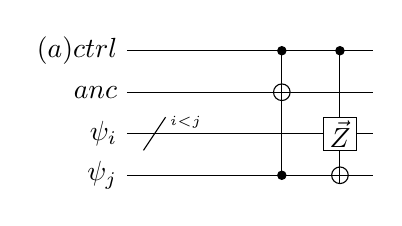
\begin{tikzpicture}[scale=1.000000,x=1pt,y=1pt]
\filldraw[color=white] (0.000000, -7.500000) rectangle (89.000000, 52.500000);
% Drawing wires
% Line 1: ctrl W \text{(a) }ctrl
\draw[color=black] (0.000000,45.000000) -- (89.000000,45.000000);
\draw[color=black] (0.000000,45.000000) node[left] {$\text{(a) }ctrl$};
% Line 2: anc W anc
\draw[color=black] (0.000000,30.000000) -- (89.000000,30.000000);
\draw[color=black] (0.000000,30.000000) node[left] {$anc$};
% Line 3: i W \psi_i
\draw[color=black] (0.000000,15.000000) -- (89.000000,15.000000);
\draw[color=black] (0.000000,15.000000) node[left] {$\psi_i$};
% Line 4: j W \psi_j
\draw[color=black] (0.000000,0.000000) -- (89.000000,0.000000);
\draw[color=black] (0.000000,0.000000) node[left] {$\psi_j$};
% Done with wires; drawing gates
% Line 6: i / ^{i<j}
\draw (6.000000, 9.000000) -- (14.000000, 21.000000);
\draw (12.000000, 18.000000) node[right] {$\scriptstyle{^{i<j}}$};
% Line 7: ctrl anc i j LABEL
% Line 8: ctrl j +anc
\draw (56.000000,45.000000) -- (56.000000,0.000000);
\filldraw (56.000000, 45.000000) circle(1.500000pt);
\filldraw (56.000000, 0.000000) circle(1.500000pt);
\begin{scope}
\draw[fill=white] (56.000000, 30.000000) circle(3.000000pt);
\clip (56.000000, 30.000000) circle(3.000000pt);
\draw (53.000000, 30.000000) -- (59.000000, 30.000000);
\draw (56.000000, 27.000000) -- (56.000000, 33.000000);
\end{scope}
% Line 10: i G $\vec{Z}$ ctrl +j
\draw (77.000000,45.000000) -- (77.000000,0.000000);
\begin{scope}
\draw[fill=white] (77.000000, 15.000000) +(-45.000000:8.485281pt and 8.485281pt) -- +(45.000000:8.485281pt and 8.485281pt) -- +(135.000000:8.485281pt and 8.485281pt) -- +(225.000000:8.485281pt and 8.485281pt) -- cycle;
\clip (77.000000, 15.000000) +(-45.000000:8.485281pt and 8.485281pt) -- +(45.000000:8.485281pt and 8.485281pt) -- +(135.000000:8.485281pt and 8.485281pt) -- +(225.000000:8.485281pt and 8.485281pt) -- cycle;
\draw (77.000000, 15.000000) node {$\vec{Z}$};
\end{scope}
\filldraw (77.000000, 45.000000) circle(1.500000pt);
\begin{scope}
\draw[fill=white] (77.000000, 0.000000) circle(3.000000pt);
\clip (77.000000, 0.000000) circle(3.000000pt);
\draw (74.000000, 0.000000) -- (80.000000, 0.000000);
\draw (77.000000, -3.000000) -- (77.000000, 3.000000);
\end{scope}
% Done with gates; drawing ending labels
% Done with ending labels; drawing cut lines and comments
% Done with comments
\end{tikzpicture}

    }
    \mbox{
        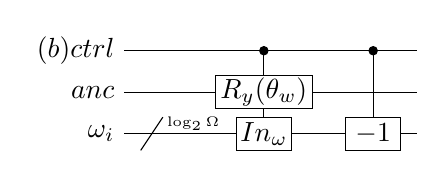
\begin{tikzpicture}[scale=1.000000,x=1pt,y=1pt]
\filldraw[color=white] (0.000000, -7.500000) rectangle (106.000000, 37.500000);
% Drawing wires
% Line 1: ctrl W \text{(b) }ctrl
\draw[color=black] (0.000000,30.000000) -- (106.000000,30.000000);
\draw[color=black] (0.000000,30.000000) node[left] {$\text{(b) }ctrl$};
% Line 2: anc W anc
\draw[color=black] (0.000000,15.000000) -- (106.000000,15.000000);
\draw[color=black] (0.000000,15.000000) node[left] {$anc$};
% Line 3: i W \omega_i
\draw[color=black] (0.000000,0.000000) -- (106.000000,0.000000);
\draw[color=black] (0.000000,0.000000) node[left] {$\omega_i$};
% Done with wires; drawing gates
% Line 5: i / ^{\log_2{\Omega}}
\draw (6.000000, -6.000000) -- (14.000000, 6.000000);
\draw (12.000000, 3.000000) node[right] {$\scriptstyle{^{\log_2{\Omega}}}$};
% Line 6: ctrl anc i LABEL width=-5
% Line 8: anc G:width=35 $R_y(\theta_w)$ i G:width=20 $In_\omega$ ctrl
\draw (50.500000,30.000000) -- (50.500000,0.000000);
\begin{scope}
\draw[fill=white] (50.500000, 15.000000) +(-45.000000:24.748737pt and 8.485281pt) -- +(45.000000:24.748737pt and 8.485281pt) -- +(135.000000:24.748737pt and 8.485281pt) -- +(225.000000:24.748737pt and 8.485281pt) -- cycle;
\clip (50.500000, 15.000000) +(-45.000000:24.748737pt and 8.485281pt) -- +(45.000000:24.748737pt and 8.485281pt) -- +(135.000000:24.748737pt and 8.485281pt) -- +(225.000000:24.748737pt and 8.485281pt) -- cycle;
\draw (50.500000, 15.000000) node {$R_y(\theta_w)$};
\end{scope}
\begin{scope}
\draw[fill=white] (50.500000, -0.000000) +(-45.000000:14.142136pt and 8.485281pt) -- +(45.000000:14.142136pt and 8.485281pt) -- +(135.000000:14.142136pt and 8.485281pt) -- +(225.000000:14.142136pt and 8.485281pt) -- cycle;
\clip (50.500000, -0.000000) +(-45.000000:14.142136pt and 8.485281pt) -- +(45.000000:14.142136pt and 8.485281pt) -- +(135.000000:14.142136pt and 8.485281pt) -- +(225.000000:14.142136pt and 8.485281pt) -- cycle;
\draw (50.500000, -0.000000) node {$In_\omega$};
\end{scope}
\filldraw (50.500000, 30.000000) circle(1.500000pt);
% Line 9: i G width=20 $-1$ ctrl
\draw (90.000000,30.000000) -- (90.000000,0.000000);
\begin{scope}
\draw[fill=white] (90.000000, -0.000000) +(-45.000000:14.142136pt and 8.485281pt) -- +(45.000000:14.142136pt and 8.485281pt) -- +(135.000000:14.142136pt and 8.485281pt) -- +(225.000000:14.142136pt and 8.485281pt) -- cycle;
\clip (90.000000, -0.000000) +(-45.000000:14.142136pt and 8.485281pt) -- +(45.000000:14.142136pt and 8.485281pt) -- +(135.000000:14.142136pt and 8.485281pt) -- +(225.000000:14.142136pt and 8.485281pt) -- cycle;
\draw (90.000000, -0.000000) node {$-1$};
\end{scope}
\filldraw (90.000000, 30.000000) circle(1.500000pt);
% Done with gates; drawing ending labels
% Done with ending labels; drawing cut lines and comments
% Done with comments
\end{tikzpicture}

    }
    \caption{
        \textbf{Bosonic Ladder Operator Block-Encoding}
        In (a), a block-encoding for the bosonic creation operator ($a_i^\dagger$) is given.
        In (b), a block-encoding for the bosonic annihilation operator ($a_i$) is given.
    }
    \label{fig:bosonic-ladder-op-be}
\end{figure}

The desired action of the block-encoding circuit for the bosonic creation operator is to increase the occupation of the bosonic mode by $1$ and rotate the block-encoding ancilla such that it has a coefficient of $\sqrt{\omega_i + 1 / \Omega}$ in the $\ket{0}$ state when the initial occupation of the $i^\text{th}$ bosonic mode is $w_i$.
This can be achieved by applying an incrementer to the the bosonic mode which increases the occupation by $1 \mod \Omega$ in each branch of the wavefunction.
The desired amplitudes of the block-encoding ancilla can be obtained using a series of $R_y$ gates that are controlled on the corresponding bosonic occupation.
An example circuit diagram is given in subfigure \ref{fig:bosonic-ladder-op-be}a.
A block-encoding for the bosonic annihilation operator can be constructed similarly, but with the block-encoding ancilla rotated prior to the occupation of the mode being decremented (subfigure \ref{fig:bosonic-ladder-op-be}b).

The angles of the $R_y$ gates are determined classically by the following function:
\begin{equation}
    \label{eq:single-op-angles}
    \theta(\omega_i) = 
    \begin{cases} 
        2 \cos^{-1}\Big(\sqrt{\omega_i/\Omega}\Big) & \text{when } \omega_i < \Omega\\
        \pi & \text{when } \omega_i = \Omega
    \end{cases}
\end{equation}
where $\omega_i$ here in comparison with $\omega_i + 1$ in Eq. \ref{eq:be-bos-creation} is due to the occupation of the state being updated prior to the controlled rotations.


An implementation of a controlled incrementer circuit is given in \cite{Gidney_2015} which requires $\lceil \log_2\Omega \rceil - 1$ clean ancillae and $3 \lceil \log_2\Omega \rceil$ T gates.
The series of uniformly controlled rotations can be decomposed via the protocol given in Möttönen et. al \cite{mottonen2004transformation}.
A discussion of different schemes to construct a \textit{controlled} set of uniformly controlled rotations is given in Appendix \ref{sec:multiplexed-rotations}.
The resource estimates quoted in the remainder of this work assume the decomposition that requires $\Omega + 3$ uncontrolled rotations and $4 \lceil{\log_2{\Omega}}\rceil$ T gates (Figure \ref{fig:gate-optimized-controlled-multiplexed-rotations}).
In total, this block-encoding has an optimal rescaling factor ($\sqrt{\Omega}$), requires one block-encoding ancilla and $\lceil{\log_2{\Omega}}\rceil$ clean ancillae, and uses $7 \lceil \log_2\Omega \rceil$ T gates and (at most) $\Omega + 3$ arbitrary rotations.


\subsection{Products of Bosonic Ladder Operators}

In this subsection, we discuss constructing block-encodings for a product of bosonic ladder operators acting on the same mode.
Unlike fermions, multiple bosons can occupy the same bosonic mode and a series of bosonic ladder operators can be applied to the state without necessarily zeroing-out the state.
Products of bosonic ladder operators acting on different modes can be block-encoded using the methods described in subsection \ref{subsec:be-products}.

Consider the desired action of a block-encoding for series of $R$ bosonic creation operators acting on the $i^\text{th}$ bosonic mode:
\begin{widetext}
\begin{equation}
    \label{eq:be-S-creation-ops}
    \begin{split}
        U_{(a^\dagger_i)^R} \ket{\psi_{i_a}} \ket{0}_\text{anc} =
        \begin{cases}
            \prod_{r=1}^{R} \sqrt{(\omega_i + r) / \Omega} \ket{\omega_i + R} \ket{0}_\text{anc} + \beta \ket{\perp} & \text{when } \omega_i \leq \Omega - R \\
            \ket{\perp} & \text{when } \omega_i > \Omega - R \\
        \end{cases}
    \end{split}
\end{equation}
\end{widetext}

\begin{figure}
    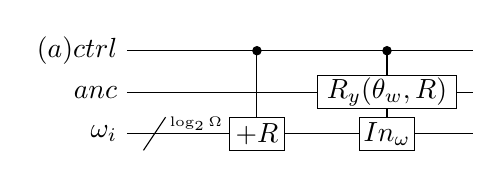
\begin{tikzpicture}[scale=1.000000,x=1pt,y=1pt]
\filldraw[color=white] (0.000000, -7.500000) rectangle (125.000000, 37.500000);
% Drawing wires
% Line 1: ctrl W \text{(a) }ctrl
\draw[color=black] (0.000000,30.000000) -- (125.000000,30.000000);
\draw[color=black] (0.000000,30.000000) node[left] {$\text{(a) }ctrl$};
% Line 2: anc W anc
\draw[color=black] (0.000000,15.000000) -- (125.000000,15.000000);
\draw[color=black] (0.000000,15.000000) node[left] {$anc$};
% Line 3: i W \omega_i
\draw[color=black] (0.000000,0.000000) -- (125.000000,0.000000);
\draw[color=black] (0.000000,0.000000) node[left] {$\omega_i$};
% Done with wires; drawing gates
% Line 5: i / ^{\log_2{\Omega}}
\draw (6.000000, -6.000000) -- (14.000000, 6.000000);
\draw (12.000000, 3.000000) node[right] {$\scriptstyle{^{\log_2{\Omega}}}$};
% Line 6: ctrl anc i LABEL width=-1
% Line 8: i G width=20 $+R$ ctrl
\draw (47.000000,30.000000) -- (47.000000,0.000000);
\begin{scope}
\draw[fill=white] (47.000000, -0.000000) +(-45.000000:14.142136pt and 8.485281pt) -- +(45.000000:14.142136pt and 8.485281pt) -- +(135.000000:14.142136pt and 8.485281pt) -- +(225.000000:14.142136pt and 8.485281pt) -- cycle;
\clip (47.000000, -0.000000) +(-45.000000:14.142136pt and 8.485281pt) -- +(45.000000:14.142136pt and 8.485281pt) -- +(135.000000:14.142136pt and 8.485281pt) -- +(225.000000:14.142136pt and 8.485281pt) -- cycle;
\draw (47.000000, -0.000000) node {$+R$};
\end{scope}
\filldraw (47.000000, 30.000000) circle(1.500000pt);
% Line 9: anc G:width=50 $R_y(\theta_w, R)$ i G:width=20 $In_\omega$ ctrl
\draw (94.000000,30.000000) -- (94.000000,0.000000);
\begin{scope}
\draw[fill=white] (94.000000, 15.000000) +(-45.000000:35.355339pt and 8.485281pt) -- +(45.000000:35.355339pt and 8.485281pt) -- +(135.000000:35.355339pt and 8.485281pt) -- +(225.000000:35.355339pt and 8.485281pt) -- cycle;
\clip (94.000000, 15.000000) +(-45.000000:35.355339pt and 8.485281pt) -- +(45.000000:35.355339pt and 8.485281pt) -- +(135.000000:35.355339pt and 8.485281pt) -- +(225.000000:35.355339pt and 8.485281pt) -- cycle;
\draw (94.000000, 15.000000) node {$R_y(\theta_w, R)$};
\end{scope}
\begin{scope}
\draw[fill=white] (94.000000, -0.000000) +(-45.000000:14.142136pt and 8.485281pt) -- +(45.000000:14.142136pt and 8.485281pt) -- +(135.000000:14.142136pt and 8.485281pt) -- +(225.000000:14.142136pt and 8.485281pt) -- cycle;
\clip (94.000000, -0.000000) +(-45.000000:14.142136pt and 8.485281pt) -- +(45.000000:14.142136pt and 8.485281pt) -- +(135.000000:14.142136pt and 8.485281pt) -- +(225.000000:14.142136pt and 8.485281pt) -- cycle;
\draw (94.000000, -0.000000) node {$In_\omega$};
\end{scope}
\filldraw (94.000000, 30.000000) circle(1.500000pt);
% Done with gates; drawing ending labels
% Done with ending labels; drawing cut lines and comments
% Done with comments
\end{tikzpicture}

    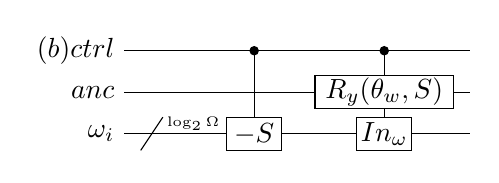
\begin{tikzpicture}[scale=1.000000,x=1pt,y=1pt]
\filldraw[color=white] (0.000000, -7.500000) rectangle (125.000000, 37.500000);
% Drawing wires
% Line 1: ctrl W \text{(b) }ctrl
\draw[color=black] (0.000000,30.000000) -- (125.000000,30.000000);
\draw[color=black] (0.000000,30.000000) node[left] {$\text{(b) }ctrl$};
% Line 2: anc W anc
\draw[color=black] (0.000000,15.000000) -- (125.000000,15.000000);
\draw[color=black] (0.000000,15.000000) node[left] {$anc$};
% Line 3: i W \omega_i
\draw[color=black] (0.000000,0.000000) -- (125.000000,0.000000);
\draw[color=black] (0.000000,0.000000) node[left] {$\omega_i$};
% Done with wires; drawing gates
% Line 5: i / ^{\log_2{\Omega}}
\draw (6.000000, -6.000000) -- (14.000000, 6.000000);
\draw (12.000000, 3.000000) node[right] {$\scriptstyle{^{\log_2{\Omega}}}$};
% Line 6: ctrl anc i LABEL width=-1
% Line 8: i G width=20 $-S$ ctrl
\draw (47.000000,30.000000) -- (47.000000,0.000000);
\begin{scope}
\draw[fill=white] (47.000000, -0.000000) +(-45.000000:14.142136pt and 8.485281pt) -- +(45.000000:14.142136pt and 8.485281pt) -- +(135.000000:14.142136pt and 8.485281pt) -- +(225.000000:14.142136pt and 8.485281pt) -- cycle;
\clip (47.000000, -0.000000) +(-45.000000:14.142136pt and 8.485281pt) -- +(45.000000:14.142136pt and 8.485281pt) -- +(135.000000:14.142136pt and 8.485281pt) -- +(225.000000:14.142136pt and 8.485281pt) -- cycle;
\draw (47.000000, -0.000000) node {$-S$};
\end{scope}
\filldraw (47.000000, 30.000000) circle(1.500000pt);
% Line 9: anc G:width=50 $R_y(\theta_w, S)$ i G:width=20 $In_\omega$ ctrl
\draw (94.000000,30.000000) -- (94.000000,0.000000);
\begin{scope}
\draw[fill=white] (94.000000, 15.000000) +(-45.000000:35.355339pt and 8.485281pt) -- +(45.000000:35.355339pt and 8.485281pt) -- +(135.000000:35.355339pt and 8.485281pt) -- +(225.000000:35.355339pt and 8.485281pt) -- cycle;
\clip (94.000000, 15.000000) +(-45.000000:35.355339pt and 8.485281pt) -- +(45.000000:35.355339pt and 8.485281pt) -- +(135.000000:35.355339pt and 8.485281pt) -- +(225.000000:35.355339pt and 8.485281pt) -- cycle;
\draw (94.000000, 15.000000) node {$R_y(\theta_w, S)$};
\end{scope}
\begin{scope}
\draw[fill=white] (94.000000, -0.000000) +(-45.000000:14.142136pt and 8.485281pt) -- +(45.000000:14.142136pt and 8.485281pt) -- +(135.000000:14.142136pt and 8.485281pt) -- +(225.000000:14.142136pt and 8.485281pt) -- cycle;
\clip (94.000000, -0.000000) +(-45.000000:14.142136pt and 8.485281pt) -- +(45.000000:14.142136pt and 8.485281pt) -- +(135.000000:14.142136pt and 8.485281pt) -- +(225.000000:14.142136pt and 8.485281pt) -- cycle;
\draw (94.000000, -0.000000) node {$In_\omega$};
\end{scope}
\filldraw (94.000000, 30.000000) circle(1.500000pt);
% Done with gates; drawing ending labels
% Done with ending labels; drawing cut lines and comments
% Done with comments
\end{tikzpicture}

    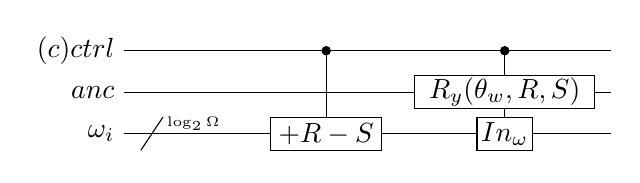
\begin{tikzpicture}[scale=1.000000,x=1pt,y=1pt]
\filldraw[color=white] (0.000000, -7.500000) rectangle (176.000000, 37.500000);
% Drawing wires
% Line 1: ctrl W \text{(c) }ctrl
\draw[color=black] (0.000000,30.000000) -- (176.000000,30.000000);
\draw[color=black] (0.000000,30.000000) node[left] {$\text{(c) }ctrl$};
% Line 2: anc W anc
\draw[color=black] (0.000000,15.000000) -- (176.000000,15.000000);
\draw[color=black] (0.000000,15.000000) node[left] {$anc$};
% Line 3: i W \omega_i
\draw[color=black] (0.000000,0.000000) -- (176.000000,0.000000);
\draw[color=black] (0.000000,0.000000) node[left] {$\omega_i$};
% Done with wires; drawing gates
% Line 5: i / ^{\log_2{\Omega}}
\draw (6.000000, -6.000000) -- (14.000000, 6.000000);
\draw (12.000000, 3.000000) node[right] {$\scriptstyle{^{\log_2{\Omega}}}$};
% Line 6: ctrl anc i LABEL
% Line 8: i G width=40 $+R-S$ ctrl
\draw (73.000000,30.000000) -- (73.000000,0.000000);
\begin{scope}
\draw[fill=white] (73.000000, -0.000000) +(-45.000000:28.284271pt and 8.485281pt) -- +(45.000000:28.284271pt and 8.485281pt) -- +(135.000000:28.284271pt and 8.485281pt) -- +(225.000000:28.284271pt and 8.485281pt) -- cycle;
\clip (73.000000, -0.000000) +(-45.000000:28.284271pt and 8.485281pt) -- +(45.000000:28.284271pt and 8.485281pt) -- +(135.000000:28.284271pt and 8.485281pt) -- +(225.000000:28.284271pt and 8.485281pt) -- cycle;
\draw (73.000000, -0.000000) node {$+R-S$};
\end{scope}
\filldraw (73.000000, 30.000000) circle(1.500000pt);
% Line 9: anc G:width=65 $R_y(\theta_w, R, S)$ i G:width=20 $In_\omega$ ctrl
\draw (137.500000,30.000000) -- (137.500000,0.000000);
\begin{scope}
\draw[fill=white] (137.500000, 15.000000) +(-45.000000:45.961941pt and 8.485281pt) -- +(45.000000:45.961941pt and 8.485281pt) -- +(135.000000:45.961941pt and 8.485281pt) -- +(225.000000:45.961941pt and 8.485281pt) -- cycle;
\clip (137.500000, 15.000000) +(-45.000000:45.961941pt and 8.485281pt) -- +(45.000000:45.961941pt and 8.485281pt) -- +(135.000000:45.961941pt and 8.485281pt) -- +(225.000000:45.961941pt and 8.485281pt) -- cycle;
\draw (137.500000, 15.000000) node {$R_y(\theta_w, R, S)$};
\end{scope}
\begin{scope}
\draw[fill=white] (137.500000, -0.000000) +(-45.000000:14.142136pt and 8.485281pt) -- +(45.000000:14.142136pt and 8.485281pt) -- +(135.000000:14.142136pt and 8.485281pt) -- +(225.000000:14.142136pt and 8.485281pt) -- cycle;
\clip (137.500000, -0.000000) +(-45.000000:14.142136pt and 8.485281pt) -- +(45.000000:14.142136pt and 8.485281pt) -- +(135.000000:14.142136pt and 8.485281pt) -- +(225.000000:14.142136pt and 8.485281pt) -- cycle;
\draw (137.500000, -0.000000) node {$In_\omega$};
\end{scope}
\filldraw (137.500000, 30.000000) circle(1.500000pt);
% Done with gates; drawing ending labels
% Done with ending labels; drawing cut lines and comments
% Done with comments
\end{tikzpicture}

    \caption{
        \textbf{Block-Encoding Product of Bosonic Ladder Operators}
        In (a), a block-encoding for the operator $(a_i^\dagger)^R$ is given.
        In (b), a block-encoding for the operator $(a_i)^S$ is given.
        In (c), a block-encoding for the operator $(a_i^\dagger)^R (a_i)^S$ is given.
    }
    \label{fig:products-bosonic-operators}
\end{figure}

A block-encoding for this operator can be achieved by updating the occupation of the bosonic mode by $+R$ and then performing a single series of rotations.
A circuit diagram for this construction is shown in subfigure \ref{fig:products-bosonic-operators}a.

The angles of the $R_y$ rotations are determined classically by the following function:
\begin{equation}
    \begin{split}
        \theta(\omega_i, R) = \\
        \begin{cases} 
            2\cos^{-1}\Big(\prod_{r=0}^{R-1}\sqrt{(\omega_i - r) / \Omega}\Big) & \text{when } \omega_i \leq \Omega - R \\
            \pi & \text{when } \omega_i > \Omega - R
        \end{cases}
    \end{split}
\end{equation}
where $\omega_i - r$ here in comparison with $\omega_i + r$ in Eq. \ref{eq:be-S-creation-ops} is due to the occupation of the state being updated prior to the controlled rotations.

A block-encoding for a bosonic annihilation operator being applied $S$ times can be achieved using a similar construction shown in subfigue \ref{fig:products-bosonic-operators}b.
The occupation of the mode is first decreased by $S$ and then the controlled multiplexed rotations are applied to pick up the corresponding coefficient on the block-encoding ancilla.
The function to determine the rotation angles is given by:
\begin{equation}
    \begin{split}
        \theta(\omega_i, S) = \\
        \begin{cases} 
            2\cos^{-1}\Big(\prod_{s=1}^{S}\sqrt{(\omega_i + s) / \Omega}\Big) & \text{when } \omega_i \geq S \\
            \pi & \text{when } \omega_i < S
        \end{cases}
    \end{split}
\end{equation}

Likewise, a block-encoding for an operator of the form $(a_i^\dagger)^R (a_i)^S$ can be constructed using a similar form (subfigue \ref{fig:products-bosonic-operators}c).
The occupation of the mode is updated by a value of $+ R - S$ and then the controlled multiplexed rotations are applied to pick up the corresponding coefficient on the block-encoding ancilla.
The function to determine the rotation angles is given by:
\begin{widetext}
\begin{equation}
    \theta(\omega_i, R, S) = 
    \begin{cases} 
        2\cos^{-1}\Big(\prod_{r=0}^{R-1}\sqrt{(\omega_i - r) / \Omega} \prod_{s=1}^{S}\sqrt{(\omega_i - R + s) / \Omega}\Big) & \text{when } S \leq \omega_i \leq \Omega - R \\
        \pi & \text{Otherwise} 
    \end{cases}
\end{equation}
\end{widetext}

Incrementing a quantum register by a classical value can be implemented in multiple ways with different implementations having different space-time tradeoffs.
The resource estimates presented in this work assume the compilation given in Figure \ref{fig:addition-gate-efficient}, which requires (at most) $3 \lceil \log_2 \Omega \rceil$ T gates.
In total, these block-encoding circuits have a rescaling factor of $\lambda = \Omega^{(R+S)/2}$, require one block-encoding ancilla and $\lceil{\log_2{\Omega}}\rceil$ clean ancillae, and use (at most) $7 \lceil \log_2 \Omega \rceil$ T gates and $\Omega + 3$ arbitrary rotations.


\subsection{Linear Combinations of Bosonic Ladder Operators}

In this subsection, we discuss constructing block-encodings for a linear combination of a product of bosonic ladder operators with its hermitian conjugate.


\begin{figure*}
    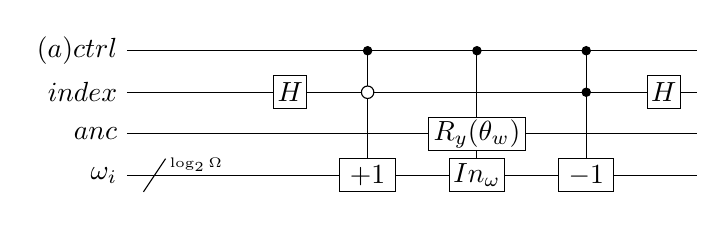
\begin{tikzpicture}[scale=1.000000,x=1pt,y=1pt]
\filldraw[color=white] (0.000000, -7.500000) rectangle (206.000000, 52.500000);
% Drawing wires
% Line 1: ctrl W \text{(a) }ctrl
\draw[color=black] (0.000000,45.000000) -- (206.000000,45.000000);
\draw[color=black] (0.000000,45.000000) node[left] {$\text{(a) }ctrl$};
% Line 2: index W index
\draw[color=black] (0.000000,30.000000) -- (206.000000,30.000000);
\draw[color=black] (0.000000,30.000000) node[left] {$index$};
% Line 3: anc W anc
\draw[color=black] (0.000000,15.000000) -- (206.000000,15.000000);
\draw[color=black] (0.000000,15.000000) node[left] {$anc$};
% Line 4: i W \omega_i
\draw[color=black] (0.000000,0.000000) -- (206.000000,0.000000);
\draw[color=black] (0.000000,0.000000) node[left] {$\omega_i$};
% Done with wires; drawing gates
% Line 6: i / ^{\log_2{\Omega}}
\draw (6.000000, -6.000000) -- (14.000000, 6.000000);
\draw (12.000000, 3.000000) node[right] {$\scriptstyle{^{\log_2{\Omega}}}$};
% Line 7: ctrl anc index i LABEL
% Line 9: index G $H$
\begin{scope}
\draw[fill=white] (59.000000, 30.000000) +(-45.000000:8.485281pt and 8.485281pt) -- +(45.000000:8.485281pt and 8.485281pt) -- +(135.000000:8.485281pt and 8.485281pt) -- +(225.000000:8.485281pt and 8.485281pt) -- cycle;
\clip (59.000000, 30.000000) +(-45.000000:8.485281pt and 8.485281pt) -- +(45.000000:8.485281pt and 8.485281pt) -- +(135.000000:8.485281pt and 8.485281pt) -- +(225.000000:8.485281pt and 8.485281pt) -- cycle;
\draw (59.000000, 30.000000) node {$H$};
\end{scope}
% Line 10: i G width=20 $+1$ ctrl -index
\draw (87.000000,45.000000) -- (87.000000,0.000000);
\begin{scope}
\draw[fill=white] (87.000000, -0.000000) +(-45.000000:14.142136pt and 8.485281pt) -- +(45.000000:14.142136pt and 8.485281pt) -- +(135.000000:14.142136pt and 8.485281pt) -- +(225.000000:14.142136pt and 8.485281pt) -- cycle;
\clip (87.000000, -0.000000) +(-45.000000:14.142136pt and 8.485281pt) -- +(45.000000:14.142136pt and 8.485281pt) -- +(135.000000:14.142136pt and 8.485281pt) -- +(225.000000:14.142136pt and 8.485281pt) -- cycle;
\draw (87.000000, -0.000000) node {$+1$};
\end{scope}
\filldraw (87.000000, 45.000000) circle(1.500000pt);
\draw[fill=white] (87.000000, 30.000000) circle(2.250000pt);
% Line 11: anc G:width=35 $R_y(\theta_w)$ i G:width=20 $In_\omega$ ctrl
\draw (126.500000,45.000000) -- (126.500000,0.000000);
\begin{scope}
\draw[fill=white] (126.500000, 15.000000) +(-45.000000:24.748737pt and 8.485281pt) -- +(45.000000:24.748737pt and 8.485281pt) -- +(135.000000:24.748737pt and 8.485281pt) -- +(225.000000:24.748737pt and 8.485281pt) -- cycle;
\clip (126.500000, 15.000000) +(-45.000000:24.748737pt and 8.485281pt) -- +(45.000000:24.748737pt and 8.485281pt) -- +(135.000000:24.748737pt and 8.485281pt) -- +(225.000000:24.748737pt and 8.485281pt) -- cycle;
\draw (126.500000, 15.000000) node {$R_y(\theta_w)$};
\end{scope}
\begin{scope}
\draw[fill=white] (126.500000, -0.000000) +(-45.000000:14.142136pt and 8.485281pt) -- +(45.000000:14.142136pt and 8.485281pt) -- +(135.000000:14.142136pt and 8.485281pt) -- +(225.000000:14.142136pt and 8.485281pt) -- cycle;
\clip (126.500000, -0.000000) +(-45.000000:14.142136pt and 8.485281pt) -- +(45.000000:14.142136pt and 8.485281pt) -- +(135.000000:14.142136pt and 8.485281pt) -- +(225.000000:14.142136pt and 8.485281pt) -- cycle;
\draw (126.500000, -0.000000) node {$In_\omega$};
\end{scope}
\filldraw (126.500000, 45.000000) circle(1.500000pt);
% Line 12: i G width=20 $-1$ ctrl index
\draw (166.000000,45.000000) -- (166.000000,0.000000);
\begin{scope}
\draw[fill=white] (166.000000, -0.000000) +(-45.000000:14.142136pt and 8.485281pt) -- +(45.000000:14.142136pt and 8.485281pt) -- +(135.000000:14.142136pt and 8.485281pt) -- +(225.000000:14.142136pt and 8.485281pt) -- cycle;
\clip (166.000000, -0.000000) +(-45.000000:14.142136pt and 8.485281pt) -- +(45.000000:14.142136pt and 8.485281pt) -- +(135.000000:14.142136pt and 8.485281pt) -- +(225.000000:14.142136pt and 8.485281pt) -- cycle;
\draw (166.000000, -0.000000) node {$-1$};
\end{scope}
\filldraw (166.000000, 45.000000) circle(1.500000pt);
\filldraw (166.000000, 30.000000) circle(1.500000pt);
% Line 13: index G $H$
\begin{scope}
\draw[fill=white] (194.000000, 30.000000) +(-45.000000:8.485281pt and 8.485281pt) -- +(45.000000:8.485281pt and 8.485281pt) -- +(135.000000:8.485281pt and 8.485281pt) -- +(225.000000:8.485281pt and 8.485281pt) -- cycle;
\clip (194.000000, 30.000000) +(-45.000000:8.485281pt and 8.485281pt) -- +(45.000000:8.485281pt and 8.485281pt) -- +(135.000000:8.485281pt and 8.485281pt) -- +(225.000000:8.485281pt and 8.485281pt) -- cycle;
\draw (194.000000, 30.000000) node {$H$};
\end{scope}
% Done with gates; drawing ending labels
% Done with ending labels; drawing cut lines and comments
% Done with comments
\end{tikzpicture}

    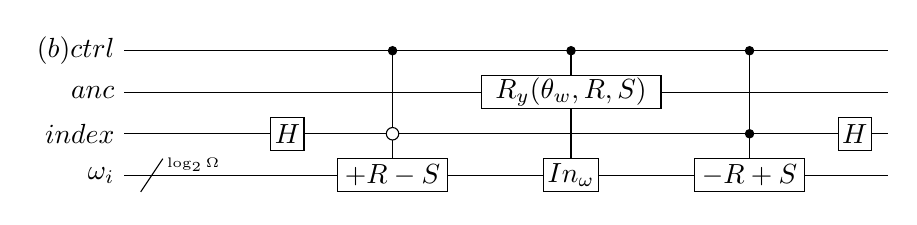
\begin{tikzpicture}[scale=1.000000,x=1pt,y=1pt]
\filldraw[color=white] (0.000000, -7.500000) rectangle (276.000000, 52.500000);
% Drawing wires
% Line 1: ctrl W \text{(b) }ctrl
\draw[color=black] (0.000000,45.000000) -- (276.000000,45.000000);
\draw[color=black] (0.000000,45.000000) node[left] {$\text{(b) }ctrl$};
% Line 2: anc W anc
\draw[color=black] (0.000000,30.000000) -- (276.000000,30.000000);
\draw[color=black] (0.000000,30.000000) node[left] {$anc$};
% Line 3: index W index
\draw[color=black] (0.000000,15.000000) -- (276.000000,15.000000);
\draw[color=black] (0.000000,15.000000) node[left] {$index$};
% Line 4: i W \omega_i
\draw[color=black] (0.000000,0.000000) -- (276.000000,0.000000);
\draw[color=black] (0.000000,0.000000) node[left] {$\omega_i$};
% Done with wires; drawing gates
% Line 6: i / ^{\log_2{\Omega}}
\draw (6.000000, -6.000000) -- (14.000000, 6.000000);
\draw (12.000000, 3.000000) node[right] {$\scriptstyle{^{\log_2{\Omega}}}$};
% Line 7: ctrl anc index i LABEL
% Line 9: index G $H$
\begin{scope}
\draw[fill=white] (59.000000, 15.000000) +(-45.000000:8.485281pt and 8.485281pt) -- +(45.000000:8.485281pt and 8.485281pt) -- +(135.000000:8.485281pt and 8.485281pt) -- +(225.000000:8.485281pt and 8.485281pt) -- cycle;
\clip (59.000000, 15.000000) +(-45.000000:8.485281pt and 8.485281pt) -- +(45.000000:8.485281pt and 8.485281pt) -- +(135.000000:8.485281pt and 8.485281pt) -- +(225.000000:8.485281pt and 8.485281pt) -- cycle;
\draw (59.000000, 15.000000) node {$H$};
\end{scope}
% Line 10: i G width=40 $+R-S$ ctrl -index
\draw (97.000000,45.000000) -- (97.000000,0.000000);
\begin{scope}
\draw[fill=white] (97.000000, -0.000000) +(-45.000000:28.284271pt and 8.485281pt) -- +(45.000000:28.284271pt and 8.485281pt) -- +(135.000000:28.284271pt and 8.485281pt) -- +(225.000000:28.284271pt and 8.485281pt) -- cycle;
\clip (97.000000, -0.000000) +(-45.000000:28.284271pt and 8.485281pt) -- +(45.000000:28.284271pt and 8.485281pt) -- +(135.000000:28.284271pt and 8.485281pt) -- +(225.000000:28.284271pt and 8.485281pt) -- cycle;
\draw (97.000000, -0.000000) node {$+R-S$};
\end{scope}
\filldraw (97.000000, 45.000000) circle(1.500000pt);
\draw[fill=white] (97.000000, 15.000000) circle(2.250000pt);
% Line 11: anc G:width=65 $R_y(\theta_w, R, S)$ i G:width=20 $In_\omega$ ctrl
\draw (161.500000,45.000000) -- (161.500000,0.000000);
\begin{scope}
\draw[fill=white] (161.500000, 30.000000) +(-45.000000:45.961941pt and 8.485281pt) -- +(45.000000:45.961941pt and 8.485281pt) -- +(135.000000:45.961941pt and 8.485281pt) -- +(225.000000:45.961941pt and 8.485281pt) -- cycle;
\clip (161.500000, 30.000000) +(-45.000000:45.961941pt and 8.485281pt) -- +(45.000000:45.961941pt and 8.485281pt) -- +(135.000000:45.961941pt and 8.485281pt) -- +(225.000000:45.961941pt and 8.485281pt) -- cycle;
\draw (161.500000, 30.000000) node {$R_y(\theta_w, R, S)$};
\end{scope}
\begin{scope}
\draw[fill=white] (161.500000, -0.000000) +(-45.000000:14.142136pt and 8.485281pt) -- +(45.000000:14.142136pt and 8.485281pt) -- +(135.000000:14.142136pt and 8.485281pt) -- +(225.000000:14.142136pt and 8.485281pt) -- cycle;
\clip (161.500000, -0.000000) +(-45.000000:14.142136pt and 8.485281pt) -- +(45.000000:14.142136pt and 8.485281pt) -- +(135.000000:14.142136pt and 8.485281pt) -- +(225.000000:14.142136pt and 8.485281pt) -- cycle;
\draw (161.500000, -0.000000) node {$In_\omega$};
\end{scope}
\filldraw (161.500000, 45.000000) circle(1.500000pt);
% Line 12: i G width=40 $-R+S$ ctrl index
\draw (226.000000,45.000000) -- (226.000000,0.000000);
\begin{scope}
\draw[fill=white] (226.000000, -0.000000) +(-45.000000:28.284271pt and 8.485281pt) -- +(45.000000:28.284271pt and 8.485281pt) -- +(135.000000:28.284271pt and 8.485281pt) -- +(225.000000:28.284271pt and 8.485281pt) -- cycle;
\clip (226.000000, -0.000000) +(-45.000000:28.284271pt and 8.485281pt) -- +(45.000000:28.284271pt and 8.485281pt) -- +(135.000000:28.284271pt and 8.485281pt) -- +(225.000000:28.284271pt and 8.485281pt) -- cycle;
\draw (226.000000, -0.000000) node {$-R+S$};
\end{scope}
\filldraw (226.000000, 45.000000) circle(1.500000pt);
\filldraw (226.000000, 15.000000) circle(1.500000pt);
% Line 13: index G $H$
\begin{scope}
\draw[fill=white] (264.000000, 15.000000) +(-45.000000:8.485281pt and 8.485281pt) -- +(45.000000:8.485281pt and 8.485281pt) -- +(135.000000:8.485281pt and 8.485281pt) -- +(225.000000:8.485281pt and 8.485281pt) -- cycle;
\clip (264.000000, 15.000000) +(-45.000000:8.485281pt and 8.485281pt) -- +(45.000000:8.485281pt and 8.485281pt) -- +(135.000000:8.485281pt and 8.485281pt) -- +(225.000000:8.485281pt and 8.485281pt) -- cycle;
\draw (264.000000, 15.000000) node {$H$};
\end{scope}
% Done with gates; drawing ending labels
% Done with ending labels; drawing cut lines and comments
% Done with comments
\end{tikzpicture}

    \caption{
        \textbf{Block-Encoding Product of Bosonic Ladder Operators Plus Hermitian Conjugate}
        In (a), a block-encoding for the operator $(a_i^\dagger + a_i)$ is given.
        In (b), a block-encoding for the operator $\big((a_i^\dagger)^R (a_i)^S + (a_i^\dagger)^S (a_i)^R\big)$ is given.
    }
    \label{fig:lc-bosonic}
\end{figure*}


Consider the block-encodings for the operators $a_i^\dagger$ and $a_i$.
An efficient block-encoding of the operator $a_i^\dagger + a_i$ can be constructed using the symmetry between the two individual block-encodings. 
To apply the creation operator, the occupancy is increased by $1$ and then the rotations are applied, whereas for the annihilation operator, the rotations are applied first and then the occupancy is decreased by $1$.
Since the desired rotation angles are independent of which operator is being applied (Eq. \ref{eq:single-op-angles}), we can apply these rotations once for both operators.
However, one additional block-encoding ancilla is required to index between the two operators.
An example circuit diagram for this construction is shown in subfigue \ref{fig:lc-bosonic}a.
A block-encoding for the generalized operator $\big((a_i^\dagger)^R (a_i)^S + (a_i^\dagger)^S (a_i)^R\big)$ can be constructed similarly and is shown in subfigure \ref{fig:lc-bosonic}b.

\begin{figure*}
    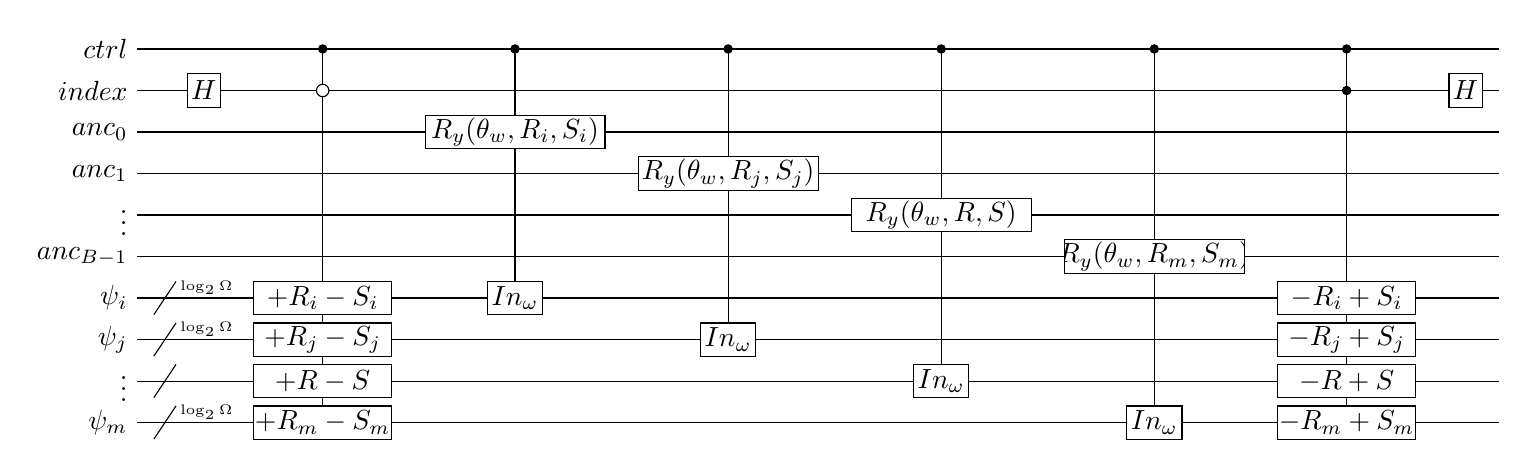
\begin{tikzpicture}[scale=1.000000,x=1pt,y=1pt]
\filldraw[color=white] (0.000000, -7.500000) rectangle (492.000000, 142.500000);
% Drawing wires
% Line 1: ctrl W ctrl
\draw[color=black] (0.000000,135.000000) -- (492.000000,135.000000);
\draw[color=black] (0.000000,135.000000) node[left] {$ctrl$};
% Line 2: index W index
\draw[color=black] (0.000000,120.000000) -- (492.000000,120.000000);
\draw[color=black] (0.000000,120.000000) node[left] {$index$};
% Line 3: anc_0 W anc_0
\draw[color=black] (0.000000,105.000000) -- (492.000000,105.000000);
\draw[color=black] (0.000000,105.000000) node[left] {$anc_0$};
% Line 4: anc_1 W anc_1
\draw[color=black] (0.000000,90.000000) -- (492.000000,90.000000);
\draw[color=black] (0.000000,90.000000) node[left] {$anc_1$};
% Line 5: anc_series W \vdots
\draw[color=black] (0.000000,75.000000) -- (492.000000,75.000000);
\draw[color=black] (0.000000,75.000000) node[left] {$\vdots$};
% Line 6: anc_B W anc_{B-1}
\draw[color=black] (0.000000,60.000000) -- (492.000000,60.000000);
\draw[color=black] (0.000000,60.000000) node[left] {$anc_{B-1}$};
% Line 8: i W \psi_i
\draw[color=black] (0.000000,45.000000) -- (492.000000,45.000000);
\draw[color=black] (0.000000,45.000000) node[left] {$\psi_i$};
% Line 9: j W \psi_j
\draw[color=black] (0.000000,30.000000) -- (492.000000,30.000000);
\draw[color=black] (0.000000,30.000000) node[left] {$\psi_j$};
% Line 10: sys_series W \vdots
\draw[color=black] (0.000000,15.000000) -- (492.000000,15.000000);
\draw[color=black] (0.000000,15.000000) node[left] {$\vdots$};
% Line 11: m W \psi_m
\draw[color=black] (0.000000,0.000000) -- (492.000000,0.000000);
\draw[color=black] (0.000000,0.000000) node[left] {$\psi_m$};
% Done with wires; drawing gates
% Line 13: i / ^{\log_2{\Omega}}
\draw (6.000000, 39.000000) -- (14.000000, 51.000000);
\draw (12.000000, 48.000000) node[right] {$\scriptstyle{^{\log_2{\Omega}}}$};
% Line 14: j / ^{\log_2{\Omega}}
\draw (6.000000, 24.000000) -- (14.000000, 36.000000);
\draw (12.000000, 33.000000) node[right] {$\scriptstyle{^{\log_2{\Omega}}}$};
% Line 15: sys_series /
\draw (6.000000, 9.000000) -- (14.000000, 21.000000);
% Line 16: m / ^{\log_2{\Omega}}
\draw (6.000000, -6.000000) -- (14.000000, 6.000000);
\draw (12.000000, 3.000000) node[right] {$\scriptstyle{^{\log_2{\Omega}}}$};
% Line 18: ctrl index anc_0 anc_1 anc_series anc_B i j sys_series m LABEL width=-20
% Line 20: index G $H$
\begin{scope}
\draw[fill=white] (24.000000, 120.000000) +(-45.000000:8.485281pt and 8.485281pt) -- +(45.000000:8.485281pt and 8.485281pt) -- +(135.000000:8.485281pt and 8.485281pt) -- +(225.000000:8.485281pt and 8.485281pt) -- cycle;
\clip (24.000000, 120.000000) +(-45.000000:8.485281pt and 8.485281pt) -- +(45.000000:8.485281pt and 8.485281pt) -- +(135.000000:8.485281pt and 8.485281pt) -- +(225.000000:8.485281pt and 8.485281pt) -- cycle;
\draw (24.000000, 120.000000) node {$H$};
\end{scope}
% Line 22: i G width=50 $+R_i-S_i$ j G width=50 $+R_j-S_j$ sys_series G width=50 $+R-S$ m G width=50 $+R_m-S_m$ ctrl -index
\draw (67.000000,135.000000) -- (67.000000,0.000000);
\begin{scope}
\draw[fill=white] (67.000000, 45.000000) +(-45.000000:35.355339pt and 8.485281pt) -- +(45.000000:35.355339pt and 8.485281pt) -- +(135.000000:35.355339pt and 8.485281pt) -- +(225.000000:35.355339pt and 8.485281pt) -- cycle;
\clip (67.000000, 45.000000) +(-45.000000:35.355339pt and 8.485281pt) -- +(45.000000:35.355339pt and 8.485281pt) -- +(135.000000:35.355339pt and 8.485281pt) -- +(225.000000:35.355339pt and 8.485281pt) -- cycle;
\draw (67.000000, 45.000000) node {$+R_i-S_i$};
\end{scope}
\begin{scope}
\draw[fill=white] (67.000000, 30.000000) +(-45.000000:35.355339pt and 8.485281pt) -- +(45.000000:35.355339pt and 8.485281pt) -- +(135.000000:35.355339pt and 8.485281pt) -- +(225.000000:35.355339pt and 8.485281pt) -- cycle;
\clip (67.000000, 30.000000) +(-45.000000:35.355339pt and 8.485281pt) -- +(45.000000:35.355339pt and 8.485281pt) -- +(135.000000:35.355339pt and 8.485281pt) -- +(225.000000:35.355339pt and 8.485281pt) -- cycle;
\draw (67.000000, 30.000000) node {$+R_j-S_j$};
\end{scope}
\begin{scope}
\draw[fill=white] (67.000000, 15.000000) +(-45.000000:35.355339pt and 8.485281pt) -- +(45.000000:35.355339pt and 8.485281pt) -- +(135.000000:35.355339pt and 8.485281pt) -- +(225.000000:35.355339pt and 8.485281pt) -- cycle;
\clip (67.000000, 15.000000) +(-45.000000:35.355339pt and 8.485281pt) -- +(45.000000:35.355339pt and 8.485281pt) -- +(135.000000:35.355339pt and 8.485281pt) -- +(225.000000:35.355339pt and 8.485281pt) -- cycle;
\draw (67.000000, 15.000000) node {$+R-S$};
\end{scope}
\begin{scope}
\draw[fill=white] (67.000000, -0.000000) +(-45.000000:35.355339pt and 8.485281pt) -- +(45.000000:35.355339pt and 8.485281pt) -- +(135.000000:35.355339pt and 8.485281pt) -- +(225.000000:35.355339pt and 8.485281pt) -- cycle;
\clip (67.000000, -0.000000) +(-45.000000:35.355339pt and 8.485281pt) -- +(45.000000:35.355339pt and 8.485281pt) -- +(135.000000:35.355339pt and 8.485281pt) -- +(225.000000:35.355339pt and 8.485281pt) -- cycle;
\draw (67.000000, -0.000000) node {$+R_m-S_m$};
\end{scope}
\filldraw (67.000000, 135.000000) circle(1.500000pt);
\draw[fill=white] (67.000000, 120.000000) circle(2.250000pt);
% Line 24: anc_0 G:width=65 $R_y(\theta_w, R_i, S_i)$ i G:width=20 $In_\omega$ ctrl
\draw (136.500000,135.000000) -- (136.500000,45.000000);
\begin{scope}
\draw[fill=white] (136.500000, 105.000000) +(-45.000000:45.961941pt and 8.485281pt) -- +(45.000000:45.961941pt and 8.485281pt) -- +(135.000000:45.961941pt and 8.485281pt) -- +(225.000000:45.961941pt and 8.485281pt) -- cycle;
\clip (136.500000, 105.000000) +(-45.000000:45.961941pt and 8.485281pt) -- +(45.000000:45.961941pt and 8.485281pt) -- +(135.000000:45.961941pt and 8.485281pt) -- +(225.000000:45.961941pt and 8.485281pt) -- cycle;
\draw (136.500000, 105.000000) node {$R_y(\theta_w, R_i, S_i)$};
\end{scope}
\begin{scope}
\draw[fill=white] (136.500000, 45.000000) +(-45.000000:14.142136pt and 8.485281pt) -- +(45.000000:14.142136pt and 8.485281pt) -- +(135.000000:14.142136pt and 8.485281pt) -- +(225.000000:14.142136pt and 8.485281pt) -- cycle;
\clip (136.500000, 45.000000) +(-45.000000:14.142136pt and 8.485281pt) -- +(45.000000:14.142136pt and 8.485281pt) -- +(135.000000:14.142136pt and 8.485281pt) -- +(225.000000:14.142136pt and 8.485281pt) -- cycle;
\draw (136.500000, 45.000000) node {$In_\omega$};
\end{scope}
\filldraw (136.500000, 135.000000) circle(1.500000pt);
% Line 25: anc_1 G:width=65 $R_y(\theta_w, R_j, S_j)$ j G:width=20 $In_\omega$ ctrl
\draw (213.500000,135.000000) -- (213.500000,30.000000);
\begin{scope}
\draw[fill=white] (213.500000, 90.000000) +(-45.000000:45.961941pt and 8.485281pt) -- +(45.000000:45.961941pt and 8.485281pt) -- +(135.000000:45.961941pt and 8.485281pt) -- +(225.000000:45.961941pt and 8.485281pt) -- cycle;
\clip (213.500000, 90.000000) +(-45.000000:45.961941pt and 8.485281pt) -- +(45.000000:45.961941pt and 8.485281pt) -- +(135.000000:45.961941pt and 8.485281pt) -- +(225.000000:45.961941pt and 8.485281pt) -- cycle;
\draw (213.500000, 90.000000) node {$R_y(\theta_w, R_j, S_j)$};
\end{scope}
\begin{scope}
\draw[fill=white] (213.500000, 30.000000) +(-45.000000:14.142136pt and 8.485281pt) -- +(45.000000:14.142136pt and 8.485281pt) -- +(135.000000:14.142136pt and 8.485281pt) -- +(225.000000:14.142136pt and 8.485281pt) -- cycle;
\clip (213.500000, 30.000000) +(-45.000000:14.142136pt and 8.485281pt) -- +(45.000000:14.142136pt and 8.485281pt) -- +(135.000000:14.142136pt and 8.485281pt) -- +(225.000000:14.142136pt and 8.485281pt) -- cycle;
\draw (213.500000, 30.000000) node {$In_\omega$};
\end{scope}
\filldraw (213.500000, 135.000000) circle(1.500000pt);
% Line 26: anc_series G:width=65 $R_y(\theta_w, R, S)$ sys_series G:width=20 $In_\omega$ ctrl
\draw (290.500000,135.000000) -- (290.500000,15.000000);
\begin{scope}
\draw[fill=white] (290.500000, 75.000000) +(-45.000000:45.961941pt and 8.485281pt) -- +(45.000000:45.961941pt and 8.485281pt) -- +(135.000000:45.961941pt and 8.485281pt) -- +(225.000000:45.961941pt and 8.485281pt) -- cycle;
\clip (290.500000, 75.000000) +(-45.000000:45.961941pt and 8.485281pt) -- +(45.000000:45.961941pt and 8.485281pt) -- +(135.000000:45.961941pt and 8.485281pt) -- +(225.000000:45.961941pt and 8.485281pt) -- cycle;
\draw (290.500000, 75.000000) node {$R_y(\theta_w, R, S)$};
\end{scope}
\begin{scope}
\draw[fill=white] (290.500000, 15.000000) +(-45.000000:14.142136pt and 8.485281pt) -- +(45.000000:14.142136pt and 8.485281pt) -- +(135.000000:14.142136pt and 8.485281pt) -- +(225.000000:14.142136pt and 8.485281pt) -- cycle;
\clip (290.500000, 15.000000) +(-45.000000:14.142136pt and 8.485281pt) -- +(45.000000:14.142136pt and 8.485281pt) -- +(135.000000:14.142136pt and 8.485281pt) -- +(225.000000:14.142136pt and 8.485281pt) -- cycle;
\draw (290.500000, 15.000000) node {$In_\omega$};
\end{scope}
\filldraw (290.500000, 135.000000) circle(1.500000pt);
% Line 27: anc_B G:width=65 $R_y(\theta_w, R_m, S_m)$ m G:width=20 $In_\omega$ ctrl
\draw (367.500000,135.000000) -- (367.500000,0.000000);
\begin{scope}
\draw[fill=white] (367.500000, 60.000000) +(-45.000000:45.961941pt and 8.485281pt) -- +(45.000000:45.961941pt and 8.485281pt) -- +(135.000000:45.961941pt and 8.485281pt) -- +(225.000000:45.961941pt and 8.485281pt) -- cycle;
\clip (367.500000, 60.000000) +(-45.000000:45.961941pt and 8.485281pt) -- +(45.000000:45.961941pt and 8.485281pt) -- +(135.000000:45.961941pt and 8.485281pt) -- +(225.000000:45.961941pt and 8.485281pt) -- cycle;
\draw (367.500000, 60.000000) node {$R_y(\theta_w, R_m, S_m)$};
\end{scope}
\begin{scope}
\draw[fill=white] (367.500000, -0.000000) +(-45.000000:14.142136pt and 8.485281pt) -- +(45.000000:14.142136pt and 8.485281pt) -- +(135.000000:14.142136pt and 8.485281pt) -- +(225.000000:14.142136pt and 8.485281pt) -- cycle;
\clip (367.500000, -0.000000) +(-45.000000:14.142136pt and 8.485281pt) -- +(45.000000:14.142136pt and 8.485281pt) -- +(135.000000:14.142136pt and 8.485281pt) -- +(225.000000:14.142136pt and 8.485281pt) -- cycle;
\draw (367.500000, -0.000000) node {$In_\omega$};
\end{scope}
\filldraw (367.500000, 135.000000) circle(1.500000pt);
% Line 29: i G width=50 $-R_i+S_i$ j G width=50 $-R_j+S_j$ sys_series G width=50 $-R+S$ m G width=50 $-R_m+S_m$ ctrl index
\draw (437.000000,135.000000) -- (437.000000,0.000000);
\begin{scope}
\draw[fill=white] (437.000000, 45.000000) +(-45.000000:35.355339pt and 8.485281pt) -- +(45.000000:35.355339pt and 8.485281pt) -- +(135.000000:35.355339pt and 8.485281pt) -- +(225.000000:35.355339pt and 8.485281pt) -- cycle;
\clip (437.000000, 45.000000) +(-45.000000:35.355339pt and 8.485281pt) -- +(45.000000:35.355339pt and 8.485281pt) -- +(135.000000:35.355339pt and 8.485281pt) -- +(225.000000:35.355339pt and 8.485281pt) -- cycle;
\draw (437.000000, 45.000000) node {$-R_i+S_i$};
\end{scope}
\begin{scope}
\draw[fill=white] (437.000000, 30.000000) +(-45.000000:35.355339pt and 8.485281pt) -- +(45.000000:35.355339pt and 8.485281pt) -- +(135.000000:35.355339pt and 8.485281pt) -- +(225.000000:35.355339pt and 8.485281pt) -- cycle;
\clip (437.000000, 30.000000) +(-45.000000:35.355339pt and 8.485281pt) -- +(45.000000:35.355339pt and 8.485281pt) -- +(135.000000:35.355339pt and 8.485281pt) -- +(225.000000:35.355339pt and 8.485281pt) -- cycle;
\draw (437.000000, 30.000000) node {$-R_j+S_j$};
\end{scope}
\begin{scope}
\draw[fill=white] (437.000000, 15.000000) +(-45.000000:35.355339pt and 8.485281pt) -- +(45.000000:35.355339pt and 8.485281pt) -- +(135.000000:35.355339pt and 8.485281pt) -- +(225.000000:35.355339pt and 8.485281pt) -- cycle;
\clip (437.000000, 15.000000) +(-45.000000:35.355339pt and 8.485281pt) -- +(45.000000:35.355339pt and 8.485281pt) -- +(135.000000:35.355339pt and 8.485281pt) -- +(225.000000:35.355339pt and 8.485281pt) -- cycle;
\draw (437.000000, 15.000000) node {$-R+S$};
\end{scope}
\begin{scope}
\draw[fill=white] (437.000000, -0.000000) +(-45.000000:35.355339pt and 8.485281pt) -- +(45.000000:35.355339pt and 8.485281pt) -- +(135.000000:35.355339pt and 8.485281pt) -- +(225.000000:35.355339pt and 8.485281pt) -- cycle;
\clip (437.000000, -0.000000) +(-45.000000:35.355339pt and 8.485281pt) -- +(45.000000:35.355339pt and 8.485281pt) -- +(135.000000:35.355339pt and 8.485281pt) -- +(225.000000:35.355339pt and 8.485281pt) -- cycle;
\draw (437.000000, -0.000000) node {$-R_m+S_m$};
\end{scope}
\filldraw (437.000000, 135.000000) circle(1.500000pt);
\filldraw (437.000000, 120.000000) circle(1.500000pt);
% Line 31: index G $H$
\begin{scope}
\draw[fill=white] (480.000000, 120.000000) +(-45.000000:8.485281pt and 8.485281pt) -- +(45.000000:8.485281pt and 8.485281pt) -- +(135.000000:8.485281pt and 8.485281pt) -- +(225.000000:8.485281pt and 8.485281pt) -- cycle;
\clip (480.000000, 120.000000) +(-45.000000:8.485281pt and 8.485281pt) -- +(45.000000:8.485281pt and 8.485281pt) -- +(135.000000:8.485281pt and 8.485281pt) -- +(225.000000:8.485281pt and 8.485281pt) -- cycle;
\draw (480.000000, 120.000000) node {$H$};
\end{scope}
% Done with gates; drawing ending labels
% Done with ending labels; drawing cut lines and comments
% Done with comments
\end{tikzpicture}

    \caption{
        \textbf{Generalized Block-Encoding Product of Bosonic Ladder Operators Plus Hermitian Conjugate}
        A block-encoding for the operator $((a_i^\dagger)^{R_i} + a_i^{S_i})((a_j^\dagger)^{R_j} + a_j^{S_j})...((a_m^\dagger)^{R_m} + a_m^{S_m}) + h.c.$ is given.
    }
    \label{fig:lc-bosonic-general}
\end{figure*}

Likewise, this construction can be generalized to a linear combination of a product of bosonic operators acting on different modes plus its hermitian conjugate.
An example circuit diagram for this construction is shown in Figure \ref{fig:lc-bosonic-general}.
For an operator acting on $B$ bosonic modes, these block-encodings have a rescaling factor of $\lambda = 2 \Omega^{P/2}$ where $P$ is the sum of the exponents of the operators in a term: $P = \sum_{b=0}^{B-1}(R_b+S_b)$.
Additionally, they require $B+1$ block-encoding ancillae and $\lceil{\log_2{\Omega}}\rceil + 1$ clean ancillae, and use (at most) \ws{double check this} $12B \lceil \log_2 \Omega \rceil - 4(B - 1)$ T gates and $B(\Omega + 3)$ arbitrary rotations.


\subsection{Terms with Fermionic and Bosonic Ladder Operators}

In the previous subsections, we discussed strategies for compiling block-encodings of different operators acting on either fermionic or bosonic modes.
In this subsection, we discuss block-encodings for operators that contain operators that act on both fermionic and bosonic operators.

\begin{figure*}
    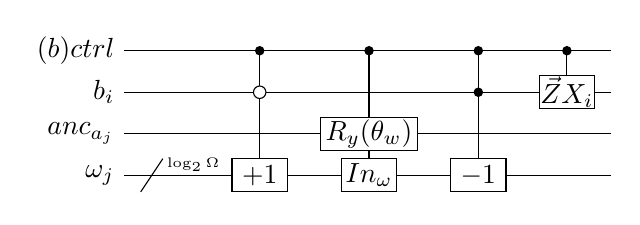
\begin{tikzpicture}[scale=1.000000,x=1pt,y=1pt]
\filldraw[color=white] (0.000000, -7.500000) rectangle (176.000000, 52.500000);
% Drawing wires
% Line 1: ctrl W \text{(b) }ctrl
\draw[color=black] (0.000000,45.000000) -- (176.000000,45.000000);
\draw[color=black] (0.000000,45.000000) node[left] {$\text{(b) }ctrl$};
% Line 2: i W b_i
\draw[color=black] (0.000000,30.000000) -- (176.000000,30.000000);
\draw[color=black] (0.000000,30.000000) node[left] {$b_i$};
% Line 3: anc_a W anc_{a_j}
\draw[color=black] (0.000000,15.000000) -- (176.000000,15.000000);
\draw[color=black] (0.000000,15.000000) node[left] {$anc_{a_j}$};
% Line 4: j W \omega_j
\draw[color=black] (0.000000,0.000000) -- (176.000000,0.000000);
\draw[color=black] (0.000000,0.000000) node[left] {$\omega_j$};
% Done with wires; drawing gates
% Line 6: j / ^{\log_2{\Omega}}
\draw (6.000000, -6.000000) -- (14.000000, 6.000000);
\draw (12.000000, 3.000000) node[right] {$\scriptstyle{^{\log_2{\Omega}}}$};
% Line 7: ctrl i anc_a j LABEL width=1
% Line 9: j G width=20 $+1$ ctrl -i
\draw (49.000000,45.000000) -- (49.000000,0.000000);
\begin{scope}
\draw[fill=white] (49.000000, -0.000000) +(-45.000000:14.142136pt and 8.485281pt) -- +(45.000000:14.142136pt and 8.485281pt) -- +(135.000000:14.142136pt and 8.485281pt) -- +(225.000000:14.142136pt and 8.485281pt) -- cycle;
\clip (49.000000, -0.000000) +(-45.000000:14.142136pt and 8.485281pt) -- +(45.000000:14.142136pt and 8.485281pt) -- +(135.000000:14.142136pt and 8.485281pt) -- +(225.000000:14.142136pt and 8.485281pt) -- cycle;
\draw (49.000000, -0.000000) node {$+1$};
\end{scope}
\filldraw (49.000000, 45.000000) circle(1.500000pt);
\draw[fill=white] (49.000000, 30.000000) circle(2.250000pt);
% Line 10: anc_a G:width=35 $R_y(\theta_w)$ j G:width=20 $In_\omega$ ctrl
\draw (88.500000,45.000000) -- (88.500000,0.000000);
\begin{scope}
\draw[fill=white] (88.500000, 15.000000) +(-45.000000:24.748737pt and 8.485281pt) -- +(45.000000:24.748737pt and 8.485281pt) -- +(135.000000:24.748737pt and 8.485281pt) -- +(225.000000:24.748737pt and 8.485281pt) -- cycle;
\clip (88.500000, 15.000000) +(-45.000000:24.748737pt and 8.485281pt) -- +(45.000000:24.748737pt and 8.485281pt) -- +(135.000000:24.748737pt and 8.485281pt) -- +(225.000000:24.748737pt and 8.485281pt) -- cycle;
\draw (88.500000, 15.000000) node {$R_y(\theta_w)$};
\end{scope}
\begin{scope}
\draw[fill=white] (88.500000, -0.000000) +(-45.000000:14.142136pt and 8.485281pt) -- +(45.000000:14.142136pt and 8.485281pt) -- +(135.000000:14.142136pt and 8.485281pt) -- +(225.000000:14.142136pt and 8.485281pt) -- cycle;
\clip (88.500000, -0.000000) +(-45.000000:14.142136pt and 8.485281pt) -- +(45.000000:14.142136pt and 8.485281pt) -- +(135.000000:14.142136pt and 8.485281pt) -- +(225.000000:14.142136pt and 8.485281pt) -- cycle;
\draw (88.500000, -0.000000) node {$In_\omega$};
\end{scope}
\filldraw (88.500000, 45.000000) circle(1.500000pt);
% Line 11: j G width=20 $-1$ ctrl i
\draw (128.000000,45.000000) -- (128.000000,0.000000);
\begin{scope}
\draw[fill=white] (128.000000, -0.000000) +(-45.000000:14.142136pt and 8.485281pt) -- +(45.000000:14.142136pt and 8.485281pt) -- +(135.000000:14.142136pt and 8.485281pt) -- +(225.000000:14.142136pt and 8.485281pt) -- cycle;
\clip (128.000000, -0.000000) +(-45.000000:14.142136pt and 8.485281pt) -- +(45.000000:14.142136pt and 8.485281pt) -- +(135.000000:14.142136pt and 8.485281pt) -- +(225.000000:14.142136pt and 8.485281pt) -- cycle;
\draw (128.000000, -0.000000) node {$-1$};
\end{scope}
\filldraw (128.000000, 45.000000) circle(1.500000pt);
\filldraw (128.000000, 30.000000) circle(1.500000pt);
% Line 13: i G width=20 $\vec{Z}X_i$ ctrl
\draw (160.000000,45.000000) -- (160.000000,30.000000);
\begin{scope}
\draw[fill=white] (160.000000, 30.000000) +(-45.000000:14.142136pt and 8.485281pt) -- +(45.000000:14.142136pt and 8.485281pt) -- +(135.000000:14.142136pt and 8.485281pt) -- +(225.000000:14.142136pt and 8.485281pt) -- cycle;
\clip (160.000000, 30.000000) +(-45.000000:14.142136pt and 8.485281pt) -- +(45.000000:14.142136pt and 8.485281pt) -- +(135.000000:14.142136pt and 8.485281pt) -- +(225.000000:14.142136pt and 8.485281pt) -- cycle;
\draw (160.000000, 30.000000) node {$\vec{Z}X_i$};
\end{scope}
\filldraw (160.000000, 45.000000) circle(1.500000pt);
% Done with gates; drawing ending labels
% Done with ending labels; drawing cut lines and comments
% Done with comments
\end{tikzpicture}

    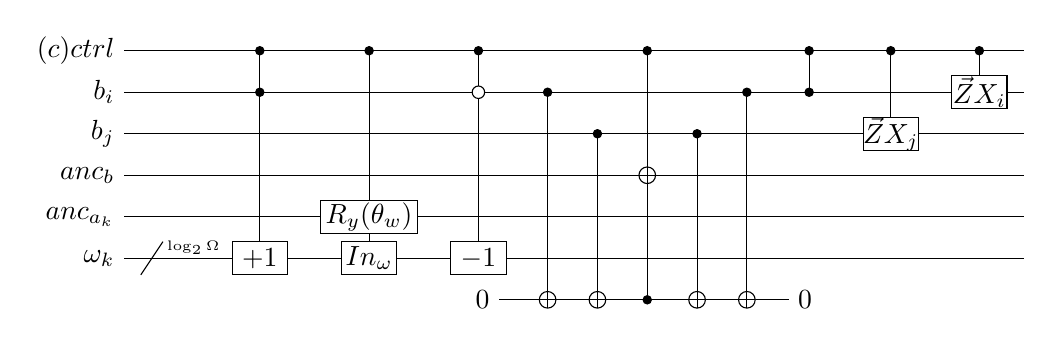
\begin{tikzpicture}[scale=1.000000,x=1pt,y=1pt]
\filldraw[color=white] (0.000000, -7.500000) rectangle (325.000000, 97.500000);
% Drawing wires
% Line 1: ctrl W \text{(c) }ctrl
\draw[color=black] (0.000000,90.000000) -- (325.000000,90.000000);
\draw[color=black] (0.000000,90.000000) node[left] {$\text{(c) }ctrl$};
% Line 2: i W b_i
\draw[color=black] (0.000000,75.000000) -- (325.000000,75.000000);
\draw[color=black] (0.000000,75.000000) node[left] {$b_i$};
% Line 3: j W b_j
\draw[color=black] (0.000000,60.000000) -- (325.000000,60.000000);
\draw[color=black] (0.000000,60.000000) node[left] {$b_j$};
% Line 4: anc_b W anc_b
\draw[color=black] (0.000000,45.000000) -- (325.000000,45.000000);
\draw[color=black] (0.000000,45.000000) node[left] {$anc_b$};
% Line 5: anc_a W anc_{a_k}
\draw[color=black] (0.000000,30.000000) -- (325.000000,30.000000);
\draw[color=black] (0.000000,30.000000) node[left] {$anc_{a_k}$};
% Line 6: k W \omega_k
\draw[color=black] (0.000000,15.000000) -- (325.000000,15.000000);
\draw[color=black] (0.000000,15.000000) node[left] {$\omega_k$};
% Line 7: c0 W 0 0
\draw[color=black] (128.000000,0.000000) -- (247.500000,0.000000);
% Done with wires; drawing gates
% Line 9: k / ^{\log_2{\Omega}}
\draw (6.000000, 9.000000) -- (14.000000, 21.000000);
\draw (12.000000, 18.000000) node[right] {$\scriptstyle{^{\log_2{\Omega}}}$};
% Line 10: ctrl i j anc_b anc_a k c0 LABEL width=1
% Line 12: k G width=20 $+1$ ctrl i
\draw (49.000000,90.000000) -- (49.000000,15.000000);
\begin{scope}
\draw[fill=white] (49.000000, 15.000000) +(-45.000000:14.142136pt and 8.485281pt) -- +(45.000000:14.142136pt and 8.485281pt) -- +(135.000000:14.142136pt and 8.485281pt) -- +(225.000000:14.142136pt and 8.485281pt) -- cycle;
\clip (49.000000, 15.000000) +(-45.000000:14.142136pt and 8.485281pt) -- +(45.000000:14.142136pt and 8.485281pt) -- +(135.000000:14.142136pt and 8.485281pt) -- +(225.000000:14.142136pt and 8.485281pt) -- cycle;
\draw (49.000000, 15.000000) node {$+1$};
\end{scope}
\filldraw (49.000000, 90.000000) circle(1.500000pt);
\filldraw (49.000000, 75.000000) circle(1.500000pt);
% Line 13: anc_a G:width=35 $R_y(\theta_w)$ k G:width=20 $In_\omega$ ctrl
\draw (88.500000,90.000000) -- (88.500000,15.000000);
\begin{scope}
\draw[fill=white] (88.500000, 30.000000) +(-45.000000:24.748737pt and 8.485281pt) -- +(45.000000:24.748737pt and 8.485281pt) -- +(135.000000:24.748737pt and 8.485281pt) -- +(225.000000:24.748737pt and 8.485281pt) -- cycle;
\clip (88.500000, 30.000000) +(-45.000000:24.748737pt and 8.485281pt) -- +(45.000000:24.748737pt and 8.485281pt) -- +(135.000000:24.748737pt and 8.485281pt) -- +(225.000000:24.748737pt and 8.485281pt) -- cycle;
\draw (88.500000, 30.000000) node {$R_y(\theta_w)$};
\end{scope}
\begin{scope}
\draw[fill=white] (88.500000, 15.000000) +(-45.000000:14.142136pt and 8.485281pt) -- +(45.000000:14.142136pt and 8.485281pt) -- +(135.000000:14.142136pt and 8.485281pt) -- +(225.000000:14.142136pt and 8.485281pt) -- cycle;
\clip (88.500000, 15.000000) +(-45.000000:14.142136pt and 8.485281pt) -- +(45.000000:14.142136pt and 8.485281pt) -- +(135.000000:14.142136pt and 8.485281pt) -- +(225.000000:14.142136pt and 8.485281pt) -- cycle;
\draw (88.500000, 15.000000) node {$In_\omega$};
\end{scope}
\filldraw (88.500000, 90.000000) circle(1.500000pt);
% Line 14: k G width=20 $-1$ ctrl -i
\draw (128.000000,90.000000) -- (128.000000,15.000000);
\begin{scope}
\draw[fill=white] (128.000000, 15.000000) +(-45.000000:14.142136pt and 8.485281pt) -- +(45.000000:14.142136pt and 8.485281pt) -- +(135.000000:14.142136pt and 8.485281pt) -- +(225.000000:14.142136pt and 8.485281pt) -- cycle;
\clip (128.000000, 15.000000) +(-45.000000:14.142136pt and 8.485281pt) -- +(45.000000:14.142136pt and 8.485281pt) -- +(135.000000:14.142136pt and 8.485281pt) -- +(225.000000:14.142136pt and 8.485281pt) -- cycle;
\draw (128.000000, 15.000000) node {$-1$};
\end{scope}
\filldraw (128.000000, 90.000000) circle(1.500000pt);
\draw[fill=white] (128.000000, 75.000000) circle(2.250000pt);
% Line 16: c0 START
\draw[color=black] (135.500000,0.000000) node[fill=white,left,minimum height=15.000000pt,minimum width=15.000000pt,inner sep=0pt] {\phantom{$0$}};
\draw[color=black] (135.500000,0.000000) node[left] {$0$};
% Line 17: i +c0
\draw (153.000000,75.000000) -- (153.000000,0.000000);
\filldraw (153.000000, 75.000000) circle(1.500000pt);
\begin{scope}
\draw[fill=white] (153.000000, 0.000000) circle(3.000000pt);
\clip (153.000000, 0.000000) circle(3.000000pt);
\draw (150.000000, 0.000000) -- (156.000000, 0.000000);
\draw (153.000000, -3.000000) -- (153.000000, 3.000000);
\end{scope}
% Line 18: j +c0
\draw (171.000000,60.000000) -- (171.000000,0.000000);
\filldraw (171.000000, 60.000000) circle(1.500000pt);
\begin{scope}
\draw[fill=white] (171.000000, 0.000000) circle(3.000000pt);
\clip (171.000000, 0.000000) circle(3.000000pt);
\draw (168.000000, 0.000000) -- (174.000000, 0.000000);
\draw (171.000000, -3.000000) -- (171.000000, 3.000000);
\end{scope}
% Line 19: ctrl c0 +anc_b
\draw (189.000000,90.000000) -- (189.000000,0.000000);
\filldraw (189.000000, 90.000000) circle(1.500000pt);
\filldraw (189.000000, 0.000000) circle(1.500000pt);
\begin{scope}
\draw[fill=white] (189.000000, 45.000000) circle(3.000000pt);
\clip (189.000000, 45.000000) circle(3.000000pt);
\draw (186.000000, 45.000000) -- (192.000000, 45.000000);
\draw (189.000000, 42.000000) -- (189.000000, 48.000000);
\end{scope}
% Line 20: j +c0
\draw (207.000000,60.000000) -- (207.000000,0.000000);
\filldraw (207.000000, 60.000000) circle(1.500000pt);
\begin{scope}
\draw[fill=white] (207.000000, 0.000000) circle(3.000000pt);
\clip (207.000000, 0.000000) circle(3.000000pt);
\draw (204.000000, 0.000000) -- (210.000000, 0.000000);
\draw (207.000000, -3.000000) -- (207.000000, 3.000000);
\end{scope}
% Line 21: i +c0
\draw (225.000000,75.000000) -- (225.000000,0.000000);
\filldraw (225.000000, 75.000000) circle(1.500000pt);
\begin{scope}
\draw[fill=white] (225.000000, 0.000000) circle(3.000000pt);
\clip (225.000000, 0.000000) circle(3.000000pt);
\draw (222.000000, 0.000000) -- (228.000000, 0.000000);
\draw (225.000000, -3.000000) -- (225.000000, 3.000000);
\end{scope}
% Line 22: c0 END
\draw[color=black] (240.000000,0.000000) node[fill=white,right,minimum height=15.000000pt,minimum width=15.000000pt,inner sep=0pt] {\phantom{$0$}};
\draw[color=black] (240.000000,0.000000) node[right] {$0$};
% Line 24: ctrl i
\draw (247.500000,90.000000) -- (247.500000,75.000000);
\filldraw (247.500000, 90.000000) circle(1.500000pt);
\filldraw (247.500000, 75.000000) circle(1.500000pt);
% Line 26: j G width=20 $\vec{Z}X_j$ ctrl
\draw (277.000000,90.000000) -- (277.000000,60.000000);
\begin{scope}
\draw[fill=white] (277.000000, 60.000000) +(-45.000000:14.142136pt and 8.485281pt) -- +(45.000000:14.142136pt and 8.485281pt) -- +(135.000000:14.142136pt and 8.485281pt) -- +(225.000000:14.142136pt and 8.485281pt) -- cycle;
\clip (277.000000, 60.000000) +(-45.000000:14.142136pt and 8.485281pt) -- +(45.000000:14.142136pt and 8.485281pt) -- +(135.000000:14.142136pt and 8.485281pt) -- +(225.000000:14.142136pt and 8.485281pt) -- cycle;
\draw (277.000000, 60.000000) node {$\vec{Z}X_j$};
\end{scope}
\filldraw (277.000000, 90.000000) circle(1.500000pt);
% Line 27: i G width=20 $\vec{Z}X_i$ ctrl
\draw (309.000000,90.000000) -- (309.000000,75.000000);
\begin{scope}
\draw[fill=white] (309.000000, 75.000000) +(-45.000000:14.142136pt and 8.485281pt) -- +(45.000000:14.142136pt and 8.485281pt) -- +(135.000000:14.142136pt and 8.485281pt) -- +(225.000000:14.142136pt and 8.485281pt) -- cycle;
\clip (309.000000, 75.000000) +(-45.000000:14.142136pt and 8.485281pt) -- +(45.000000:14.142136pt and 8.485281pt) -- +(135.000000:14.142136pt and 8.485281pt) -- +(225.000000:14.142136pt and 8.485281pt) -- cycle;
\draw (309.000000, 75.000000) node {$\vec{Z}X_i$};
\end{scope}
\filldraw (309.000000, 90.000000) circle(1.500000pt);
% Done with gates; drawing ending labels
% Done with ending labels; drawing cut lines and comments
% Done with comments
\end{tikzpicture}

    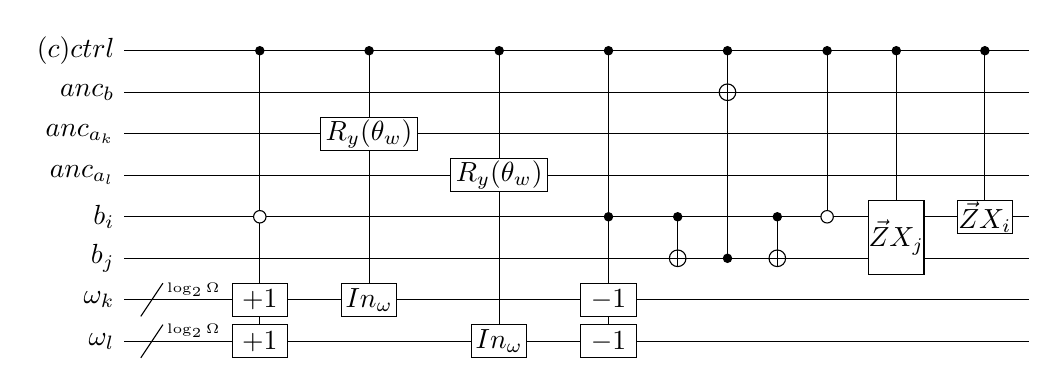
\begin{tikzpicture}[scale=1.000000,x=1pt,y=1pt]
\filldraw[color=white] (0.000000, -7.500000) rectangle (327.000000, 112.500000);
% Drawing wires
% Line 1: ctrl W \text{(c) }ctrl
\draw[color=black] (0.000000,105.000000) -- (327.000000,105.000000);
\draw[color=black] (0.000000,105.000000) node[left] {$\text{(c) }ctrl$};
% Line 2: anc_b W anc_b
\draw[color=black] (0.000000,90.000000) -- (327.000000,90.000000);
\draw[color=black] (0.000000,90.000000) node[left] {$anc_b$};
% Line 3: anc_k W anc_{a_k}
\draw[color=black] (0.000000,75.000000) -- (327.000000,75.000000);
\draw[color=black] (0.000000,75.000000) node[left] {$anc_{a_k}$};
% Line 4: anc_l W anc_{a_l}
\draw[color=black] (0.000000,60.000000) -- (327.000000,60.000000);
\draw[color=black] (0.000000,60.000000) node[left] {$anc_{a_l}$};
% Line 5: i W b_i
\draw[color=black] (0.000000,45.000000) -- (327.000000,45.000000);
\draw[color=black] (0.000000,45.000000) node[left] {$b_i$};
% Line 6: j W b_j
\draw[color=black] (0.000000,30.000000) -- (327.000000,30.000000);
\draw[color=black] (0.000000,30.000000) node[left] {$b_j$};
% Line 7: k W \omega_k
\draw[color=black] (0.000000,15.000000) -- (327.000000,15.000000);
\draw[color=black] (0.000000,15.000000) node[left] {$\omega_k$};
% Line 8: l W \omega_l
\draw[color=black] (0.000000,0.000000) -- (327.000000,0.000000);
\draw[color=black] (0.000000,0.000000) node[left] {$\omega_l$};
% Done with wires; drawing gates
% Line 10: k / ^{\log_2{\Omega}}
\draw (6.000000, 9.000000) -- (14.000000, 21.000000);
\draw (12.000000, 18.000000) node[right] {$\scriptstyle{^{\log_2{\Omega}}}$};
% Line 11: l / ^{\log_2{\Omega}}
\draw (6.000000, -6.000000) -- (14.000000, 6.000000);
\draw (12.000000, 3.000000) node[right] {$\scriptstyle{^{\log_2{\Omega}}}$};
% Line 12: ctrl i j anc_b anc_k anc_l k l LABEL width=1
% Line 14: k G width=20 $+1$ l G width=20 $+1$ ctrl -i
\draw (49.000000,105.000000) -- (49.000000,0.000000);
\begin{scope}
\draw[fill=white] (49.000000, 15.000000) +(-45.000000:14.142136pt and 8.485281pt) -- +(45.000000:14.142136pt and 8.485281pt) -- +(135.000000:14.142136pt and 8.485281pt) -- +(225.000000:14.142136pt and 8.485281pt) -- cycle;
\clip (49.000000, 15.000000) +(-45.000000:14.142136pt and 8.485281pt) -- +(45.000000:14.142136pt and 8.485281pt) -- +(135.000000:14.142136pt and 8.485281pt) -- +(225.000000:14.142136pt and 8.485281pt) -- cycle;
\draw (49.000000, 15.000000) node {$+1$};
\end{scope}
\begin{scope}
\draw[fill=white] (49.000000, -0.000000) +(-45.000000:14.142136pt and 8.485281pt) -- +(45.000000:14.142136pt and 8.485281pt) -- +(135.000000:14.142136pt and 8.485281pt) -- +(225.000000:14.142136pt and 8.485281pt) -- cycle;
\clip (49.000000, -0.000000) +(-45.000000:14.142136pt and 8.485281pt) -- +(45.000000:14.142136pt and 8.485281pt) -- +(135.000000:14.142136pt and 8.485281pt) -- +(225.000000:14.142136pt and 8.485281pt) -- cycle;
\draw (49.000000, -0.000000) node {$+1$};
\end{scope}
\filldraw (49.000000, 105.000000) circle(1.500000pt);
\draw[fill=white] (49.000000, 45.000000) circle(2.250000pt);
% Line 15: anc_k G:width=35 $R_y(\theta_w)$ k G:width=20 $In_\omega$ ctrl
\draw (88.500000,105.000000) -- (88.500000,15.000000);
\begin{scope}
\draw[fill=white] (88.500000, 75.000000) +(-45.000000:24.748737pt and 8.485281pt) -- +(45.000000:24.748737pt and 8.485281pt) -- +(135.000000:24.748737pt and 8.485281pt) -- +(225.000000:24.748737pt and 8.485281pt) -- cycle;
\clip (88.500000, 75.000000) +(-45.000000:24.748737pt and 8.485281pt) -- +(45.000000:24.748737pt and 8.485281pt) -- +(135.000000:24.748737pt and 8.485281pt) -- +(225.000000:24.748737pt and 8.485281pt) -- cycle;
\draw (88.500000, 75.000000) node {$R_y(\theta_w)$};
\end{scope}
\begin{scope}
\draw[fill=white] (88.500000, 15.000000) +(-45.000000:14.142136pt and 8.485281pt) -- +(45.000000:14.142136pt and 8.485281pt) -- +(135.000000:14.142136pt and 8.485281pt) -- +(225.000000:14.142136pt and 8.485281pt) -- cycle;
\clip (88.500000, 15.000000) +(-45.000000:14.142136pt and 8.485281pt) -- +(45.000000:14.142136pt and 8.485281pt) -- +(135.000000:14.142136pt and 8.485281pt) -- +(225.000000:14.142136pt and 8.485281pt) -- cycle;
\draw (88.500000, 15.000000) node {$In_\omega$};
\end{scope}
\filldraw (88.500000, 105.000000) circle(1.500000pt);
% Line 16: anc_l G:width=35 $R_y(\theta_w)$ l G:width=20 $In_\omega$ ctrl
\draw (135.500000,105.000000) -- (135.500000,0.000000);
\begin{scope}
\draw[fill=white] (135.500000, 60.000000) +(-45.000000:24.748737pt and 8.485281pt) -- +(45.000000:24.748737pt and 8.485281pt) -- +(135.000000:24.748737pt and 8.485281pt) -- +(225.000000:24.748737pt and 8.485281pt) -- cycle;
\clip (135.500000, 60.000000) +(-45.000000:24.748737pt and 8.485281pt) -- +(45.000000:24.748737pt and 8.485281pt) -- +(135.000000:24.748737pt and 8.485281pt) -- +(225.000000:24.748737pt and 8.485281pt) -- cycle;
\draw (135.500000, 60.000000) node {$R_y(\theta_w)$};
\end{scope}
\begin{scope}
\draw[fill=white] (135.500000, -0.000000) +(-45.000000:14.142136pt and 8.485281pt) -- +(45.000000:14.142136pt and 8.485281pt) -- +(135.000000:14.142136pt and 8.485281pt) -- +(225.000000:14.142136pt and 8.485281pt) -- cycle;
\clip (135.500000, -0.000000) +(-45.000000:14.142136pt and 8.485281pt) -- +(45.000000:14.142136pt and 8.485281pt) -- +(135.000000:14.142136pt and 8.485281pt) -- +(225.000000:14.142136pt and 8.485281pt) -- cycle;
\draw (135.500000, -0.000000) node {$In_\omega$};
\end{scope}
\filldraw (135.500000, 105.000000) circle(1.500000pt);
% Line 17: k G width=20 $-1$ l G width=20 $-1$ ctrl i
\draw (175.000000,105.000000) -- (175.000000,0.000000);
\begin{scope}
\draw[fill=white] (175.000000, 15.000000) +(-45.000000:14.142136pt and 8.485281pt) -- +(45.000000:14.142136pt and 8.485281pt) -- +(135.000000:14.142136pt and 8.485281pt) -- +(225.000000:14.142136pt and 8.485281pt) -- cycle;
\clip (175.000000, 15.000000) +(-45.000000:14.142136pt and 8.485281pt) -- +(45.000000:14.142136pt and 8.485281pt) -- +(135.000000:14.142136pt and 8.485281pt) -- +(225.000000:14.142136pt and 8.485281pt) -- cycle;
\draw (175.000000, 15.000000) node {$-1$};
\end{scope}
\begin{scope}
\draw[fill=white] (175.000000, -0.000000) +(-45.000000:14.142136pt and 8.485281pt) -- +(45.000000:14.142136pt and 8.485281pt) -- +(135.000000:14.142136pt and 8.485281pt) -- +(225.000000:14.142136pt and 8.485281pt) -- cycle;
\clip (175.000000, -0.000000) +(-45.000000:14.142136pt and 8.485281pt) -- +(45.000000:14.142136pt and 8.485281pt) -- +(135.000000:14.142136pt and 8.485281pt) -- +(225.000000:14.142136pt and 8.485281pt) -- cycle;
\draw (175.000000, -0.000000) node {$-1$};
\end{scope}
\filldraw (175.000000, 105.000000) circle(1.500000pt);
\filldraw (175.000000, 45.000000) circle(1.500000pt);
% Line 19: i +j
\draw (200.000000,45.000000) -- (200.000000,30.000000);
\filldraw (200.000000, 45.000000) circle(1.500000pt);
\begin{scope}
\draw[fill=white] (200.000000, 30.000000) circle(3.000000pt);
\clip (200.000000, 30.000000) circle(3.000000pt);
\draw (197.000000, 30.000000) -- (203.000000, 30.000000);
\draw (200.000000, 27.000000) -- (200.000000, 33.000000);
\end{scope}
% Line 20: ctrl j +anc_b
\draw (218.000000,105.000000) -- (218.000000,30.000000);
\filldraw (218.000000, 105.000000) circle(1.500000pt);
\filldraw (218.000000, 30.000000) circle(1.500000pt);
\begin{scope}
\draw[fill=white] (218.000000, 90.000000) circle(3.000000pt);
\clip (218.000000, 90.000000) circle(3.000000pt);
\draw (215.000000, 90.000000) -- (221.000000, 90.000000);
\draw (218.000000, 87.000000) -- (218.000000, 93.000000);
\end{scope}
% Line 21: i +j
\draw (236.000000,45.000000) -- (236.000000,30.000000);
\filldraw (236.000000, 45.000000) circle(1.500000pt);
\begin{scope}
\draw[fill=white] (236.000000, 30.000000) circle(3.000000pt);
\clip (236.000000, 30.000000) circle(3.000000pt);
\draw (233.000000, 30.000000) -- (239.000000, 30.000000);
\draw (236.000000, 27.000000) -- (236.000000, 33.000000);
\end{scope}
% Line 23: ctrl -i
\draw (254.000000,105.000000) -- (254.000000,45.000000);
\filldraw (254.000000, 105.000000) circle(1.500000pt);
\draw[fill=white] (254.000000, 45.000000) circle(2.250000pt);
% Line 25: i j G width=20 $\vec{Z}X_j$ ctrl
\draw (279.000000,105.000000) -- (279.000000,30.000000);
\begin{scope}
\draw[fill=white] (279.000000, 37.500000) +(-45.000000:14.142136pt and 19.091883pt) -- +(45.000000:14.142136pt and 19.091883pt) -- +(135.000000:14.142136pt and 19.091883pt) -- +(225.000000:14.142136pt and 19.091883pt) -- cycle;
\clip (279.000000, 37.500000) +(-45.000000:14.142136pt and 19.091883pt) -- +(45.000000:14.142136pt and 19.091883pt) -- +(135.000000:14.142136pt and 19.091883pt) -- +(225.000000:14.142136pt and 19.091883pt) -- cycle;
\draw (279.000000, 37.500000) node {$\vec{Z}X_j$};
\end{scope}
\filldraw (279.000000, 105.000000) circle(1.500000pt);
% Line 26: i G width=20 $\vec{Z}X_i$ ctrl
\draw (311.000000,105.000000) -- (311.000000,45.000000);
\begin{scope}
\draw[fill=white] (311.000000, 45.000000) +(-45.000000:14.142136pt and 8.485281pt) -- +(45.000000:14.142136pt and 8.485281pt) -- +(135.000000:14.142136pt and 8.485281pt) -- +(225.000000:14.142136pt and 8.485281pt) -- cycle;
\clip (311.000000, 45.000000) +(-45.000000:14.142136pt and 8.485281pt) -- +(45.000000:14.142136pt and 8.485281pt) -- +(135.000000:14.142136pt and 8.485281pt) -- +(225.000000:14.142136pt and 8.485281pt) -- cycle;
\draw (311.000000, 45.000000) node {$\vec{Z}X_i$};
\end{scope}
\filldraw (311.000000, 105.000000) circle(1.500000pt);
% Done with gates; drawing ending labels
% Done with ending labels; drawing cut lines and comments
% Done with comments
\end{tikzpicture}

    \caption{
        \textbf{Block-Encoding Terms}
        In (a), a block-encoding for the operator $b_i^\dagger a_j^\dagger + a_j b_i$ is given.
        In (b), a block-encoding for the operator $ b_i^\dagger b_j^\dagger a_k^\dagger + a_k b_j b_i$ is given.
        In (c), a block-encoding for the operator $b_i^\dagger b_j^\dagger a_k^\dagger a_l^\dagger + a_l a_k b_j b_i$ is given.
    }
    \label{fig:be-term-example}
\end{figure*}


Consider the action of the operator: $b_i a_j + a_j^\dagger b_i^\dagger$ on the respective fermionic and bosonic modes.
When the fermionic mode is occupied, only the operator $b_i a_j$ will act nontrivially.
Meanwhile if the fermionic mode is unoccupied, only the operator $a_j^\dagger b_i^\dagger$ will act nontrivially.
Therefore, the occupation of the fermionic mode can be used to dictate which bosonic operator should be applied to the system.
After the appropriate bosonic operator is applied, the fermionic system is updated.
A circuit diagram for this block-encoding in given in subfigue \ref{fig:be-term-example}a.
This block-encoding circuit will have a rescaling factor of $\lambda = \sqrt{\Omega}$, requires one block-encoding ancillae and $\lceil \log_2\Omega \rceil + 1$ clean ancillae, and uses \ws{double check this} $12 \lceil \log_2 \Omega \rceil - 4$ T gates and (at most) $\Omega + 3$ arbitrary rotations.

This strategy can be employed for other combinations of bosonic and fermionic ladder operators.
In the full Yukawa model the operator $b_i^\dagger b_j^\dagger a_k^\dagger + a_k b_j b_i$ is used to model the process of a boson being annihilated to form a fermion and antifermion and a fermion and antifermion being annihilated to form a boson.
A block-encoding for this operator is shown in subfigue \ref{fig:be-term-example}b.
When constructing the circuit, the occupation of either fermionic mode can be used to determine which bosonic operator is applied to the system.
This block-encoding circuit will have a rescaling factor of $\lambda = \sqrt{\Omega}$, requires two block-encoding ancillae and $\lceil \log_2\Omega \rceil + 1$ clean ancillae, and uses \ws{double check this} $12 \lceil \log_2 \Omega \rceil$ T gates and (at most) $\Omega + 3$ arbitrary rotations.

A similar block-encoding can be constructed for the operator $b_i^\dagger b_j^\dagger a_k^\dagger a_l^\dagger + a_l a_k b_j b_i$, which appears in the full Yukawa model.
An example circuit diagram for this block-encoding is shown in subfigue \ref{fig:be-term-example}c.
This block-encoding circuit will have a rescaling factor of $\lambda = \Omega$, requires three block-encoding ancillae and $\lceil \log_2\Omega \rceil + 1$ clean ancillae, and uses \ws{double check this} $24 \lceil \log_2\Omega \rceil - 8$ T gates and (at most) $2\Omega + 6$ arbitrary rotations.

